\documentclass[11pt,twoside,a4paper,fleqn]{book} 
%\documentclass[11pt,twoside,a4paper,fleqn,draft]{book} 


%--- Packages to use
%
\usepackage[]{fancyhdr}   
\usepackage[]{natbib}
\usepackage{alltt}
\usepackage{times}
\usepackage{lscape}         % landscape mode of a single page
\usepackage[]{longtable}    % allow tables longer than one page
\usepackage{makeidx}        % index of terms
\usepackage{tabularx}       % allows line breaking in table columns
\usepackage{algorithm}      % for describing algorithms with pseudo-code
\usepackage{algorithmic}
\usepackage{ifthen}
\usepackage{ifpdf}
\usepackage{xr-hyper}
\usepackage{fancyvrb}
\usepackage{xcolor}


%--- Margins
%
\voffset-1.5cm
\headheight16pt
\headsep1.1cm
\textheight23cm
\hoffset-1.3cm
\oddsidemargin2.2cm
\textwidth14.0cm


%--- Headings
%
\pagestyle{fancy}
\renewcommand{\chaptermark}[1]{\markboth{#1}{}}
\renewcommand{\sectionmark}[1]{\markright{\thesection\ #1}}
\fancyhf{}
\fancyhead[LE,RO]{\small{\sc\thepage}}
\fancyhead[LO]{\small{\scshape\rightmark}}
\fancyhead[RE]{\small{\scshape\leftmark}}
\renewcommand{\headrulewidth}{0.5pt}
\renewcommand{\footrulewidth}{0pt}
\fancypagestyle{plain}{%
  \fancyhead{}
  \renewcommand{\headrulewidth}{0pt}
}  


%--- Some layout commands
%
\sloppy
\raggedbottom
\hbadness=10000
\makeindex
\bibliographystyle{agu}


%--- Some fixes

%- To avoid hyperref error:
\newcommand{\theHalgorithm}{\theHchapter.\arabic{algorithm}}

%- Width of the caption in longtable:
\setlength{\LTcapwidth}{0.9\textwidth} 

%- Change brace type for comments in algorithmic
\renewcommand{\algorithmiccomment}[1]{(#1)}


%--- Symbol definitions
%

% This file defines the general math macros.
% Mathematical symbols used only once, or for a particular purpose, 
% should not be included here. Note that the scalar quantities exist 
% in a subscript version, and it is not necessary to define macros for
% all possible subscripts of a variable.
% A lot of macros have been defined for the Rodgers formalism is it
% used extensively.

% If you add new definitions, please try to follow the rules below to
% get a naming scheme as consistent as possible. Just check how a 
% similar macro is defined and use it as an example.

% Patrick Eriksson 2001-03-13

%-----------------------------------------------------------------------------

% Most of the macros are named by putting 3-letters acronyms together. 
% The acronyms are mainly formed by taking the first letter and the two 
% first following consonants. The list below shows the used acronyms.
% Please, if you introduce a new acronym, add it to this list.
%
% altitude     Alt
% angel        Ang
% average      Avr
% azimuthal    Azm
% constant     Cns
% contribution Cnt
% covariance   Cvr
% derivative   Drv
% error        Err
% frequency    Frq
% forward      Frw
% function     Fnc
% identity     Idn
% inverse      Inv
% kernel       Krn
% latitude     Lat       (exception from general naming scheme)
% length       Lng
% longitude    Lon       (exception from general naming scheme)
% matrix       Mtr
% measurement  Msr
% model        Mdl
% partial      Prt
% population   Ppl
% pressure     Prs
% radius       Rds
% retrieval/ed Rtr
% sensor       Sns
% size         Sze
% space        Spc
% state        Stt
% style        Stl
% symbol       Smb
% temperature  Tmp
% transfer     Trf
% transmission Trn
% transpose    Trp
% wavelength   Wvl
% vector       Vct
% zenith       Znt
%
% a priori                              Apr
% monochromatic pencil beam intensity   Mpi
% optical thickness                     Oth
% weighting function                    Wfn

% For other terms or features, use as far as possible complete strings to get 
% macros with clear names.


%--- General math ------------------------------------------------------------

% Vector style
\newcommand{\VctStl}[1]     {\ensuremath{\mathbf{#1}}}

% Matrix style
\newcommand{\MtrStl}[1]     {\ensuremath{\mathbf{#1}}}

% The identity matrix
\newcommand{\IdnMtr}        {\MtrStl{1}}  

% Scalar or matrix inverse
\newcommand{\Inv}           {^{-1}}  

% Vector or matrix transpose
\newcommand{\Trp}           {^T}  

% Size symbol
\newcommand{\SzeSmb}        {\ensuremath{\in}}  

% Vector space
\newcommand{\VctSpc}[1]     {\ensuremath{\mathbf{R}^#1}}

% Matrix space
\newcommand{\MtrSpc}[2]     {\ensuremath{\mathbf{R}^{#1 \times #2}}}

% Vector length (simple)
\newcommand{\VctLng}        {\ensuremath{n}}  
\newcommand{\aVctLng}[1]    {\ensuremath{n_{#1}}}  

% Index (to vector, matrix ...)
\newcommand{\Ind}           {\ensuremath{i}}  
\newcommand{\aInd}[1]       {\ensuremath{i_{#1}}}  

% Differential d
\newcommand{\DiffD}         {\ensuremath{\mathrm{d}}}  

% Partial d
\newcommand{\PartD}         {\ensuremath{\partial}}  

% Real and Imaginary part
\renewcommand{\Re}            {\ensuremath{\mathrm{Re}}}
\renewcommand{\Im}            {\ensuremath{\mathrm{Im}}}

% Ensemble average
\newcommand{\EnsAvr}[1]        {\ensuremath{\left\langle #1 \right\rangle}}

% Absolute Value
\newcommand{\Abs}[1]          {\ensuremath{\left| #1 \right| }}   

% *10^#1
\newcommand{\topowerten}[1]   {\ensuremath{\cdot10^{#1}}}

% degrees
\newcommand{\degree}          {\ensuremath{^\circ}}

% 1/2
\newcommand{\half} {\ensuremath{\textstyle\frac{1}{2}}}


%--- Physical constants ------------------------------------------------------

% Speed of light in vaccum [m/s]
\newcommand{\speedoflight}   {\ensuremath{c}}  

% Planck constant [Js]
\newcommand{\planckCns}      {\ensuremath{h}}  

% Boltzmann constant [J/K]
\newcommand{\boltzmannCns}   {\ensuremath{k_b}}  

% Avogadro's number [molec/kg]
\newcommand{\avogadrosCns}   {\ensuremath{N_a}}  


%--- The Rodgers formalism ---------------------------------------------------

% True (natural) forward model
\newcommand{\trueFrwMdl}       {\ensuremath{F}}  

% Discrete forward model
\newcommand{\FrwMdl}           {\ensuremath{\mathcal{F}}}  

% Inverse model  
\newcommand{\InvMdl}           {\ensuremath{\mathcal{I}}}  

% Transfer model  
\newcommand{\TrfMdl}           {\ensuremath{\mathcal{T}}}  

% A priori symbol
\newcommand{\AprSmb}           {\ensuremath{_a}}  

% Measurement vector
\newcommand{\MsrVct}           {\VctStl{y}}  

% Vector of monochromatic pencil beam intensities
\newcommand{\MpiVct}           {\VctStl{i}}  

% Vector of monochromatic pencil beam intensities with subscript
\newcommand{\aMpiVct}[1]       {\MpiVct\ensuremath{_{#1}}}

% Measurement error vector
\newcommand{\MsrErrVct}        {\ensuremath{\varepsilon}}  

% State vector 
\newcommand{\SttVct}           {\VctStl{x}}  
\newcommand{\aSttVct}[1]       {\SttVct\ensuremath{_{#1}}}
\newcommand{\aSttVctTrp}[1]    {\SttVct\ensuremath{_{#1}\Trp}}
\newcommand{\SttElm}           {\ensuremath{x}}  
\newcommand{\aSttElm}[1]       {\SttElm\ensuremath{_{#1}}}

% A priori state vector 
\newcommand{\AprSttVct}        {\SttVct\AprSmb}

% Retrieved state vector
\newcommand{\RtrVct}           {\ensuremath{\hat{\SttVct}}}

% Forward model parameter vector
\newcommand{\FrwMdlVct}        {\VctStl{b}}  

% A priori forward model parameter vector 
\newcommand{\AprFrwMdlVct}     {\FrwMdlVct\AprSmb}

% A forward model parameters vector with subscript
\newcommand{\aFrwMdlVct}[1]    {\FrwMdlVct\ensuremath{_{#1}}}
\newcommand{\aFrwMdlVctTrp}[1] {\FrwMdlVct\ensuremath{_{#1}\Trp}}

% Inverse model parameters
\newcommand{\InvMdlVct}        {\VctStl{c}}  

% Weighting function matrix
\newcommand{\WfnMtr}           {\MtrStl{K}}
\newcommand{\aWfnMtr}[1]       {\WfnMtr\ensuremath{_{#1}}}
\newcommand{\aWfnMtrTrp}[1]    {\WfnMtr\ensuremath{_{#1}\Trp}}

% Contribution function matrix
\newcommand{\CtrFncMtr}        {\MtrStl{D_y}}  

% Averaging kernel matrix
\newcommand{\AvrKrnMtr}        {\MtrStl{A}}  
\newcommand{\aAvrKrnMtr}[1]    {\AvrKrnMtr\ensuremath{_{#1}}}

% Sensor (and data reduction) matrix
\newcommand{\SnsMtr}           {\MtrStl{H}} 
\newcommand{\aSnsMtr}[1]       {\SnsMtr\ensuremath{_{#1}}} 

% Transformation between vector spaces
\newcommand{\VctTrfMtr}        {\MtrStl{B}}  

% Covariance matrix
\newcommand{\CvrMtr}           {\MtrStl{S}}


% --- Special functions ------------------------------------------------------

% The Planck function
\newcommand{\Planck}     {\ensuremath{B}}  


% --- General scalar quantities ----------------------------------------------
%
% All quantities shall have a subscript version named as aXxx.

% Altitude (above geoid)
\newcommand{\Alt}        {\ensuremath{z}}  
\newcommand{\aAlt}[1]    {\ensuremath{z_{#1}}}

% Azimuthal angle
\newcommand{\AzmAng}     {\ensuremath{\omega}}  
\newcommand{\aAzmAng}[1] {\ensuremath{\omega_{#1}}}  

% Frequency
\newcommand{\Frq}        {\ensuremath{\nu}}  
\newcommand{\aFrq}[1]    {\ensuremath{\nu_{#1}}}  

% Wavelength
\newcommand{\Wvl}        {\ensuremath{\lambda}}  
\newcommand{\aWvl}[1]    {\ensuremath{\lambda_{#1}}}  

% Latitude
\newcommand{\Lat}        {\ensuremath{\alpha}}  
\newcommand{\aLat}[1]    {\ensuremath{\alpha_{#1}}}  

% Length along the propagation path
\newcommand{\PpathLng}        {\ensuremath{l}}  
\newcommand{\aPpathLng}[1]    {\ensuremath{l_{#1}}}  

% Longitude
\newcommand{\Lon}        {\ensuremath{\beta}}  
\newcommand{\aLon}[1]    {\ensuremath{\beta_{#1}}}  

% Monochromatic pencil beam intensity
\newcommand{\Mpi}        {\ensuremath{I}}  
\newcommand{\aMpi}[1]    {\ensuremath{I_{#1}}}  

% Optical depth
\newcommand{\Oth}        {\ensuremath{\tau}}  
\newcommand{\aOth}[1]    {\ensuremath{\tau_{#1}}}  

% Transmission
\newcommand{\Trn}        {\ensuremath{t}}  
\newcommand{\aTrn}[1]    {\ensuremath{t_{#1}}}  
\newcommand{\TrnMat}     {\MtrStl{T}}
\newcommand{\aTrnMat}[1] {\ensuremath{\MtrStl{T}_{#1}}}  

% Pressure
\newcommand{\Prs}        {\ensuremath{P}}  
\newcommand{\aPrs}[1]    {\ensuremath{P_{#1}}}  

% Pressure altitude
\newcommand{\PrsAlt}     {\ensuremath{\zeta}}  
\newcommand{\aPrsAlt}[1] {\ensuremath{\zeta_{#1}}}  

% Radius
\newcommand{\Rds}        {\ensuremath{r}}  
\newcommand{\aRds}[1]    {\ensuremath{r_{#1}}}  

% Refractive index
\newcommand{\Rfr}        {\ensuremath{n}}  
\newcommand{\aRfr}[1]    {\ensuremath{n_{#1}}}  
\newcommand{\RealRfr}    {\ensuremath{n'}}  
\newcommand{\ImagRfr}    {\ensuremath{n''}}  

% Speed
\newcommand{\Spd}        {\ensuremath{v}}  
\newcommand{\aSpd}[1]    {\ensuremath{v_{#1}}}

% Temperature
\newcommand{\Tmp}        {\ensuremath{T}}  
\newcommand{\aTmp}[1]    {\ensuremath{T_{#1}}}  

% Zenith angle
\newcommand{\ZntAng}     {\ensuremath{\psi}}  
\newcommand{\aZntAng}[1] {\ensuremath{\psi_{#1}}}  

% Winds
\newcommand{\Wind}        {\ensuremath{v}}  
\newcommand{\WindWE}      {\ensuremath{v_u}}  
\newcommand{\WindSN}      {\ensuremath{v_v}}  
\newcommand{\WindVe}      {\ensuremath{v_w}}  


% --- Radiative transfer quantities -------------------

% Stokes vector
\newcommand{\StoVec}    {\ensuremath{{\bf s}}}
\newcommand{\aStoVec}[1]{\ensuremath{{\bf s}_{#1}}}
\newcommand{\StoI}      {\ensuremath{I}}
\newcommand{\aStoI}[1]  {\ensuremath{I_{#1}}}
\newcommand{\StoQ}      {\ensuremath{Q}}
\newcommand{\aStoQ}[1]  {\ensuremath{Q_{#1}}}
\newcommand{\StoU}      {\ensuremath{U}}
\newcommand{\StoV}      {\ensuremath{V}}

% Degree of polarisation
\newcommand{\DgrPlr}      {\ensuremath{p}}

% Propagation direction and position
\newcommand{\PDir}      {\ensuremath{{\bf \hat{n}}}}
\newcommand{\PPos}      {\ensuremath{{\bf r}}}

% Total extinction matrix
\newcommand{\ExtMat}    {\ensuremath{{\bf K}}}
\newcommand{\aExtMat}[1]{\ensuremath{{\bf K}_{#1}}}

% Absorption matrix
\newcommand{\AbsMat}    {\ensuremath{{\bf A}}}
\newcommand{\aAbsMat}[1]{\ensuremath{{\bf A}_{#1}}}

% Total absorption vector
\newcommand{\AbsVec}    {\ensuremath{{\bf a}}}
\newcommand{\aAbsVec}[1]{\ensuremath{{\bf a}_{#1}}}     

% Emission source vector
\newcommand{\EmsVec}    {\ensuremath{{\bf b}}}

% Source vector
\newcommand{\SrcVec}    {\ensuremath{{\bf j}}}
\newcommand{\aSrcVec}[1]{\ensuremath{{\bf j}_{#1}}}     

% Phase matrix
\newcommand{\PhaMat}    {\ensuremath{{\bf Z}}}
\newcommand{\aPhaMat}[1]{\ensuremath{{\bf Z}_{#1}}}

% Scattering matrix
\newcommand{\ScaMat}    {\ensuremath{{\bf F}}}
\newcommand{\aScaMat}[1]{\ensuremath{{\bf F}_{#1}}}

% Particle density
\newcommand{\PDen}      {\ensuremath{n^p}}

% Radiation field
\newcommand{\IFld}      {\ensuremath{{\mathcal I}}}
% Radiation field index
\newcommand{\aIFld}[1]  {\ensuremath{{\mathcal I}^{(#1)}}}

% Scattered field
\newcommand{\SFld}      {\ensuremath{{\mathcal S}}}

% Scattered field index
\newcommand{\aSFld}[1]  {\ensuremath{{\mathcal S}^{(#1)}}}

% Scattering Integral vector
\newcommand{\SVec}      {\ensuremath{{\bf s}}}

% Amplitude matrix
\newcommand{\AmpMat}    {\ensuremath{{\bf S}}}

% Phase matrix
\newcommand{\TraMat}    {\ensuremath{{\bf T}}}
\newcommand{\aTraMat}[1]{\ensuremath{{\bf T}_{#1}}}

% Amplitude matrix index
\newcommand{\IAmp}      {\ensuremath{i_{amp}}}

% Single extinction matrix
\newcommand{\SExMat}    {\ensuremath{{\bf L}}}
\newcommand{\aSExMat}[1]{\ensuremath{{\bf L}^{#1}}}     

% Scattered field
\newcommand{\ScaInt}    {\ensuremath{{\bf S}}}

% Identity matrix
\newcommand{\IdnMat}    {\ensuremath{{\bf E}}}

% Scattering zenith angle
\newcommand{\ScaZa}     {\ensuremath{{\psi_s}}}

% Scattering azimuth angle
\newcommand{\ScaAa}     {\ensuremath{{\omega_s}}}

% Particle type index
\newcommand{\IPart}     {\ensuremath{{i_{part}}}}

%Inverse Wave Impendance
\newcommand{\InvImp} %
      {\ensuremath{\sqrt{\textstyle{\frac{\epsilon}{\mu}}}}}    

% Micrometer
\newcommand{\mum}          {\ensuremath{\mu m}}

% Incoming direction
\newcommand{\inc}       {\mathrm{inc}}

% Scattered direction
\newcommand{\sca}       {\mathrm{sca}}

% Ice mass content
\newcommand{\imc}       {\ensuremath{IMC}}

% effective radius
\newcommand{\Reff}       {\ensuremath{R_{eff}}}


% --- Quantities concerning scalar gas absorption  -------------------

% Absorption coefficient
\newcommand{\AbsCoef}    {\ensuremath{{\alpha}}}
\newcommand{\aAbsCoef}[1]{\ensuremath{{\alpha}_{#1}}}

% Total absorption coefficient
\newcommand{\AbsCoefTot} {\aAbsCoef{\mbox{\footnotesize total}}}

% Absorption cross section
\newcommand{\AbsXsec}    {\ensuremath{{\kappa}}}
\newcommand{\aAbsXsec}[1]{\ensuremath{{\kappa}_{#1}}}

% Number density:
\newcommand{\Den}    {\ensuremath{{n}}}
\newcommand{\aDen}[1]{\ensuremath{{n}_{#1}}}


% --- Intensity for different polarisation components  -------------------

\newcommand{\Iv}      {\ensuremath{I_v}}
\newcommand{\Ih}      {\ensuremath{I_h}}
\newcommand{\Ipff}    {\ensuremath{I_{+45^\circ}}}
\newcommand{\Imff}    {\ensuremath{I_{-45^\circ}}}
\newcommand{\Irhc}    {\ensuremath{I_{rhc}}}
\newcommand{\Ilhc}    {\ensuremath{I_{lhc}}}


% --- Brightness temperature  -------------------

\newcommand{\BT}      {\aTmp{B}}


%--- Plotting line styles ----------------------------------------------------

\def \lsolid     {\mbox{------}}
\def \ldashed    {\mbox{--~--~--}}
\def \ldashdot   {\mbox{--~$\cdot$~--}}
\def \ldotted    {\mbox{$\cdot~\cdot~\cdot$}}


% --- Misc  -------------------
\newcommand{\chem}[1] {{\ensuremath{\mathrm{#1}}}}





%--- PDF/LaTeX specific options
\ifpdf
  \usepackage{graphicx}    % includegraphics
  \DeclareGraphicsExtensions{.pdf}
  \usepackage{color}
  \definecolor{DarkRed}{rgb}{0.5,0,0}
  \usepackage
    [pdftex,                         % or dvips
     colorlinks=true,
     linkcolor=DarkRed,
     citecolor=DarkRed,
     urlcolor=DarkRed,
%     pdftitle={ARTS User Guide},
%     pdfauthor={The ARTS development team},
%     pdfsubject={},
%     pdfkeywords={},
%     bookmarks=true,
%     bookmarksopen=false,
%     pdfpagemode=None,
%     plainpages=false,
%     pdfpagelabels
      ]
  {hyperref}
  \setcounter{tocdepth}{3}
\else
  \usepackage{graphicx}    % includegraphics
  \DeclareGraphicsExtensions{.eps}
  \setcounter{tocdepth}{1}
\fi


%--- Command definitions -----------------------------------------------------

%- Document history
\newcommand{\starthistory} {\begin{table}[b]  \begin{tabular}{l p{11cm}} 
                             \hline {\bf History} & \\ }
\newcommand{\stophistory}  {\end{tabular} \end{table} }


%- Symbol table
\newcommand{\startsymbols} {\begin{table} \begin{center} 
                            \caption{Examples of symbols used in this chapter,
                            the corresponding notation in the ARTS source code
                            and a short description of the quantity. }
                            \begin{tabular}{l l l}
                            {\bf Here} & {\bf In ARTS} & {\bf Description} 
                            \\ \hline \\ } 
\newcommand{\stopsymbols}  {\\ \hline \end{tabular} 
                           \end{center} \end{table}}      
\newcommand{\startsymbolswithunits} 
                   {\begin{table} \begin{center} 
                            \caption{Examples of symbols used in this chapter,
                            the corresponding notation in the ARTS source code
                            and a short description of the quantity. }
                   \begin{tabular}{l l l l}
                   {\bf Here} & {\bf Unit} & {\bf In ARTS} & {\bf Description} 
                   \\ \hline \\ } 
\newcommand{\stopsymbolswithunits} {\stopsymbols}


%- Command to create link to ARTS built-in documentation. (Consider
% using \wsmindex, \wsvindex, etc., instead. They use this command
% implicitly.  But direct use may be useful if you use the same term
% several times in a short section, and don't want all of these
% occurrences to be in the index.)
% Underscores must be escaped by leading backslash!
\newcommand{\builtindoc}[1]{\href{http://arts.mi.uni-hamburg.de/docserver-stable/all/#1}{#1}}

%- Command to write an internal ARTS variable, internal function, or
% file name with special style. Anything that does not have built-in
% documentation. Also for other things that are code,
% but inside the text. Use the "code" environment for longer pieces of
% code.
% Underscores must be escaped by leading backslash!
\newcommand{\shortcode}[1]{\texttt{#1}}

%- Define verbatim environment for arts code examples.
% (For longer pieces of code, for in-text use "\shortcode".)
% This is the only code command where you do not have to escape
% underscores. 
\DefineVerbatimEnvironment{code}{Verbatim}{fontsize=\small}


%- Commands for easy indexing of terms
%
% Underscores must be escaped by leading backslash!
%
% Index command to use when text and index reference are equal. Otherwise
% the normal \index command must be used.
\newcommand{\textindex}[1]{#1\index{#1}} 
%
% Index command to make index for a workspace method. It writes out the
% function name in verbatim style and makes an index reference.
\newcommand{\wsmindex}[1]{\builtindoc{#1}\index{workspace methods!#1}} 
%
% Index command to make index for workspace variable. Works as \wsmindex.
\newcommand{\wsvindex}[1]{\builtindoc{#1}\index{workspace variables!#1}}
%
% Index command to make index for workspace agenda. Works as \wsmindex.
\newcommand{\wsaindex}[1]{\builtindoc{#1}\index{workspace agendas!#1}} 
%
% Index command to make index for a ARTS file. Works as \wsmindex.
\newcommand{\fileindex}[1]{\shortcode{#1}\index{ARTS files!#1}}
%
% Index command to make index for an internal function. Works as \wsmindex.
\newcommand{\funcindex}[1]{\shortcode{#1}\index{internal ARTS functions!#1}}
%
% Index command to make index for a ARTS data structure. Works as \wsmindex.
\newcommand{\typeindex}[1]{\shortcode{#1}\index{data types!#1}}


%- For FIXMEs:
\newcommand{\FIXME}[1]{\textcolor{gray}{\bfseries FIXME: #1}}


%- Names of the different documentation documents:
\newcommand{\user}{\emph{ARTS User Guide}}
\newcommand{\developer}{\emph{ARTS Developer Guide}}
\newcommand{\theory}{\emph{ARTS Theory}}

%------------------------------------------------------------------------------



%%% Local Variables: 
%%% mode: latex
%%% TeX-master: t
%%% End: 


% External documents for cross references:
\externaldocument[D-]{arts_developer}
\externaldocument[T-]{arts_theory}

%===   Start of report   ===================================================
\begin{document}


%--- Title page
%
% To suppress hyperref warning about duplicate page labels:
\renewcommand{\thepage}{title \arabic{page}} 

\thispagestyle{plain}
\begin{center}
  \vspace*{1cm}
  {\Huge \bf ARTS User Guide\\}
  \vspace*{1cm}
  {\large edited by \\}
  \vspace*{1cm}
  {\Large \bf Patrick Eriksson and Stefan Buehler }\\
   \vspace*{2cm}
   {\large \today\\
    ARTS Version $<$unavailable$>$ {\LaTeX} in-source built

   }
\end{center}
\vspace*{\fill}
{\normalsize \bf
  \noindent
  The content and usage of ARTS are not only described by this
  document. An overview of ARTS documentation and help features are
  given in Section~\ref{sec:concept:doc}. For continuous reports on
  changes of the source code and this user guide, subscribe to the
  ARTS developers mailing list at \url{http://www.sat.ltu.se/arts/support/}.

  We welcome gladly comments and reports on errors in the document.
  Send then an e-mail to: \verb|patrick.eriksson (at) chalmers.se| or 
  \verb|sbuehler (at) ltu.se|.

  If you use data generated by ARTS in a scientific
  publication, then please mention this and cite the most
  appropriate of the ARTS publications that are summarized on
  \url{http://www.sat.ltu.se/arts/docs/}.
}

\newpage                          
\thispagestyle{empty}
\vspace*{\fill}
\noindent
\begin{verbatim}
Copyright (C) 2000-2009
Stefan Buehler <sbuehler (at) ltu.se>
Patrick Eriksson <patrick.eriksson (at) chalmers.se>

The ARTS program is free software; you can redistribute it
and/or modify it under the terms of the GNU General Public
License as published by the Free Software Foundation; either
version 2, or (at your option) any later version.

This program is distributed in the hope that it will be
useful, but WITHOUT ANY WARRANTY; without even the implied
warranty of MERCHANTABILITY or FITNESS FOR A PARTICULAR
PURPOSE. See the GNU General Public License for more
details. 

You should have received a copy of the GNU General Public
License along with the program; if not, write to the Free
Software Foundation, Inc., 59 Temple Place - Suite 330,
Boston, MA 02111-1307, USA. 
\end{verbatim}



%--- Contributing authors -----------------------------------------------------
%
\newpage
\thispagestyle{plain}
%
\begin{center}
  {\Large \bf Contributing authors}
\end{center}
\vspace*{10mm}
\begin{tabular}{lp{10mm}l}
  \hline
  {\bf Author/email} & & {\bf Main contribution(s)} \\
  \hline
  Stefan Buehler$^a$ & & Editor, Sections \ref{sec:concept},  
  \ref{sec:absorption}, \ref{sec:development}, \ref{sec:workspace},
  \ref{sec:matpack} and \ref{sec:interpolation}.\\
  sbuehler (at) ltu.se & &        \\
  \hline
  Cory Davis$^d$ & & Section \ref{sec:montecarlo}. \\
  cory.davis (at) metservice.com & & \\
  \hline
  Mattias Ekstr\"om$^b$ & & Section \ref{sec:matpack:sparse}. \\
  \hline
  Claudia Emde$^c$ & & Sections \ref{sec:clouds}, \ref{sec:scattering},
  \ref{sec:lin_alg} and \ref{sec:rte_theory}.\\
  claudia.emde (at) dlr.de & & \\
  \hline
  Patrick Eriksson$^b$ &  & Editor, report structure, 
  Sections \ref{sec:atmosphere}, \ref{sec:rte}, \ref{sec:ppath}, \\
  patrick.eriksson (at) chalmers.se & & 
  \ref{sec:surface}, \ref{sec:batch}, \ref{sec:formalism} and 
  \ref{sec:rte_theory}.\\
  \hline
  Oliver Lemke$^a$ & & Latex fixes.\\
  olemke (at) core-dump.info & & \\
  \hline
  Christian Melsheimer$^c$ & & Section \ref{sec:polarization}.\\
  melsheimer (at) uni-bremen.de & & \\
  \hline
  Sreerekha T.R.$^c$ & & Section \ref{sec:integration}.\\
  \hline
  &&\\
\end{tabular}

\noindent
The present address is given for active contributors, while for others
the address to the institute where the work was performed is given:\\
$^a$ Department of Space Science, Lule{\aa} University of Technology, 
Box 812, SE-98128 Kiruna, Sweden. \\
$^b$ Department of Radio and Space Science, Chalmers University of Technology,
SE-41296 Gothenburg, Sweden. \\
$^c$ Institute of Environmental Physics, University of Bremen, P.O. Box 33044, 
D-28334 Bremen, Germany. \\
$^d$ Institute for Atmospheric and Environmental Science, University of 
Edinburgh, EH93JZ Edinburgh, Scotland, UK. \\


%--- Create an empty page
%
\newpage
\thispagestyle{empty}
\rule{0pt}{10pt}
\newpage

\pagenumbering{roman}
\tableofcontents

\cleardoublepage
\pagenumbering{arabic}
     

% ===========================================================================
% === The chapters
%============================================================================



\chapter{ARTS: concept and the programme}
 \label{sec:concept}

\starthistory
  050613 & Updated by Patrick Eriksson.\\
  020613 & Updated and extended by Stefan Buehler.\\
  000616 & Created by Stefan Buehler, based on my DPG2000 poster.
\stophistory


%
% Introduction
%
This section describes the basic ideas underlying the ARTS programme.
It also introduces some terminology. You should read it if you want to
understand how the program works and how it can be used efficiently.

This section is not about physics, only about ARTS as a computer
program. Refer to Section \ref{sec:fm_defs} for an introduction to the
physics of atmospheric radiative transfer and its mathematical
description in ARTS.


\section{Main components}
%----------------------
\label{sec:concept:main_components}

The most important notion in ARTS is the \textindex{workspace}. All
physical quantities (for example absorption coefficients) are
\textindex{workspace variables}. But workspace variables can also be of
a more technical nature, for example various grids. 

The program performs a calculation by executing a list of
\textindex{workspace methods}, which are specified in a
controlfile. These workspace methods take workspace variables as
input, and generate workspace variables as output. Additional
input parameters can be specified as \textindex{keyword parameters} in
the controlfile (Figure \ref{fig:method}).

\begin{figure}
  \begin{center}
    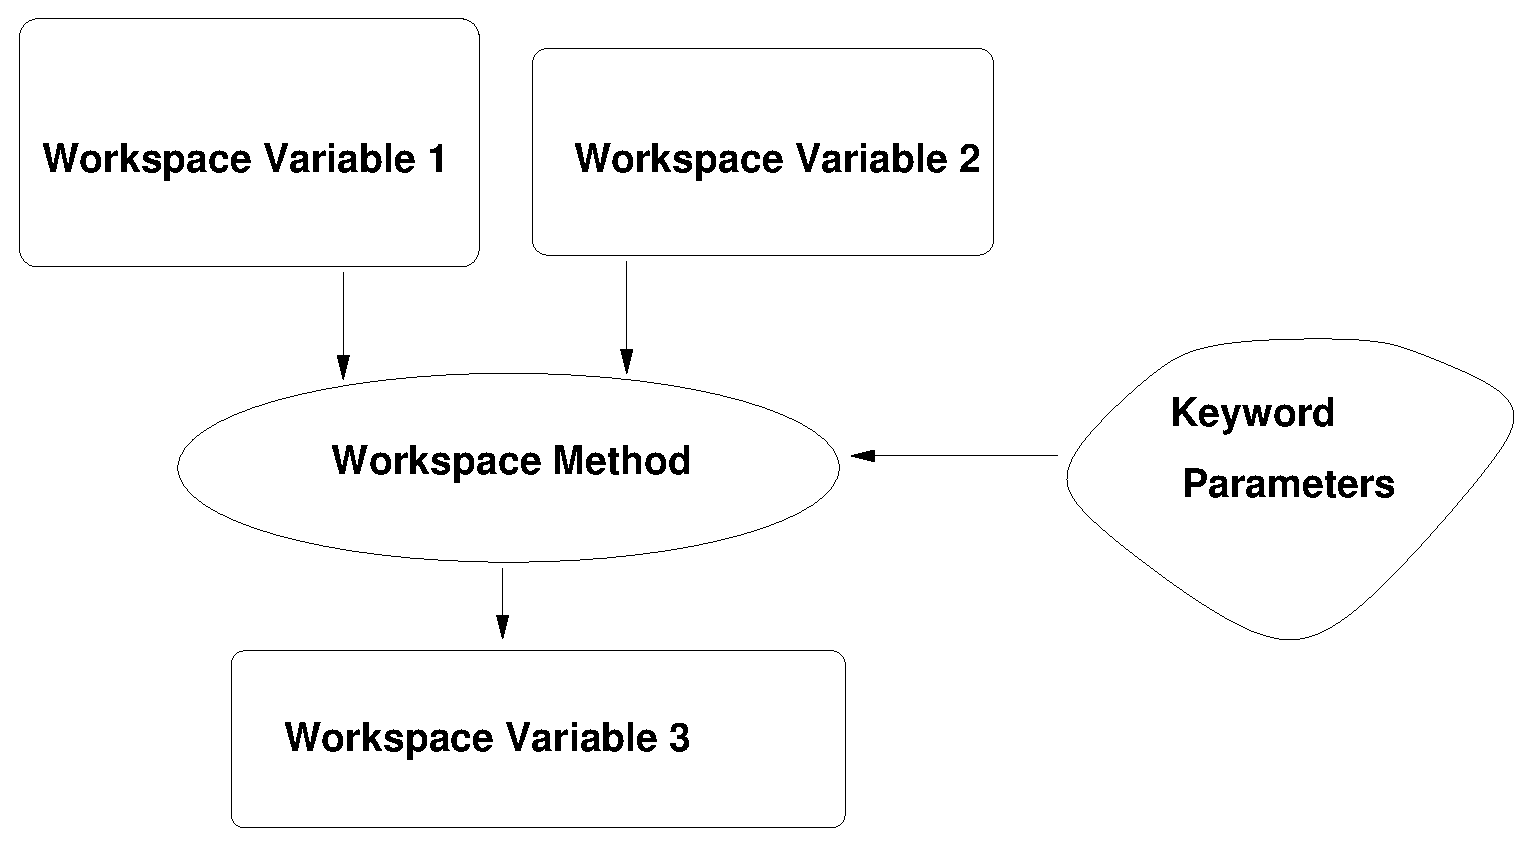
\includegraphics[width=\hsize,draft=false]{concept/method}
    \caption{\textindex{Specific
        workspace methods} act on specific workspace variables to
        generate other specific workspace variables. Additional input
        parameters can be specified as keyword parameters in the
        controlfile.}
    \label{fig:method}
  \end{center}
\end{figure}

It is important to note that the controlfile has a fixed and
well-defined syntax. This syntax is understood by the ARTS parser.
The great advantage of this concept is that it is very easy to add
new workspace variables and new workspace methods. The program has
an internal lookup table which lists all workspace methods, as well
as their input variables, output variables, and keyword
parameters. To add a new method, one just has to add an entry to
this lookup table, and write the code for the method itself. No
further changes to the program are necessary. In particular, no
changes to the program logic or to the parser. How such an extension
can be made practically is described in Section \ref{sec:development}.


\section{Generic Workspace Methods}
%=================================
\label{sec:concept:generic}

Generic methods (Figure \ref{fig:generic_method}) allow the user of
the program even more freedom than specific methods. A generic method
is for example \artsstyle{MatrixSet}, which can be used to set any
workspace variable which is a matrix. For example
\begin{quote}
  \artsstyle{MatrixSet(z\_surface){0.0}}
\end{quote}
will set all elements of \artsstyle{z\_surface} to 0.0 (as long as
\artsstyle{nrows} and \artsstyle{ncols} are set).

\begin{figure}
  \begin{center}
    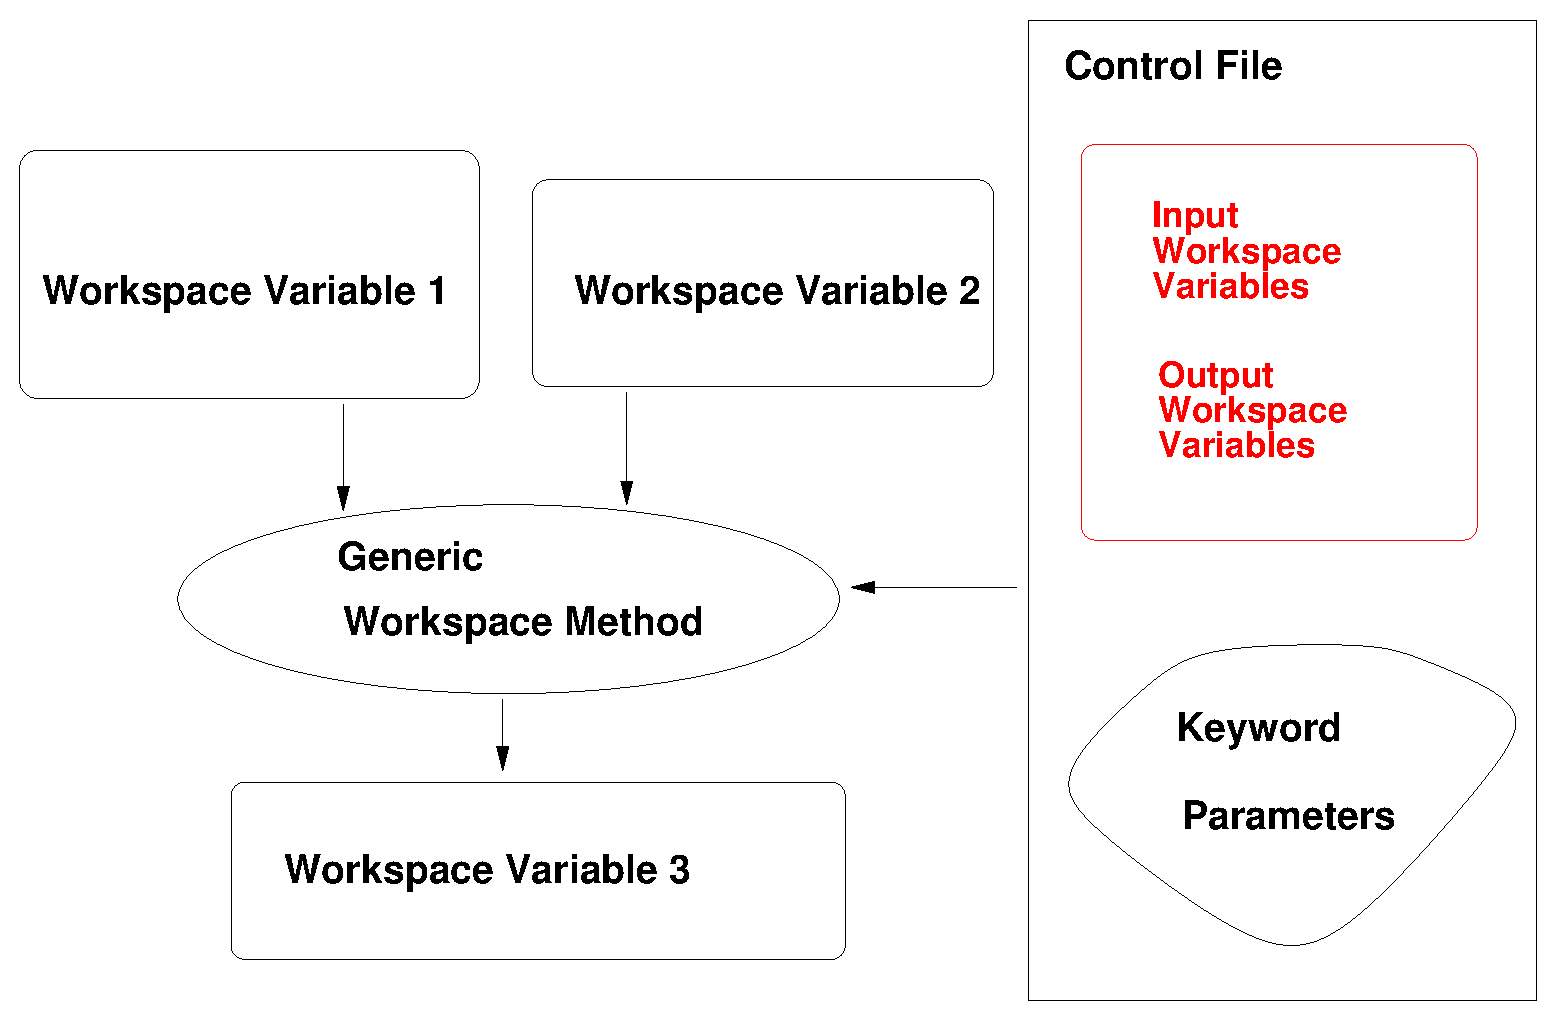
\includegraphics[width=\hsize,draft=false]{concept/generic_method}
    \caption{For \textindex{generic
      workspace methods} the workspace variables to act on are
        specified in the controlfile.}
    \label{fig:generic_method}
  \end{center}
\end{figure}

Some methods are even more flexible, the are super generic. This means
that they can take any workspace variable as input. The most commonly
used such methods are the XML file methods. A workspace variable is
read from a file in this way
\begin{quote}
  \artsstyle{ReadXML(f\_grid)\{"frequency\_grid"\}}
\end{quote}
Generic methods are particularly useful for IO operations like in the
example above. No new IO methods are necessary for new workspace
variables, as long as they are of standard types already known to the
program (for example vectors or matrices). 



\section{Agendas}
%=================================
\label{sec:concept:agendas}

Agendas are a special incarnation of a workspace method. In the
controlfile an arbitrary number of workspace methods can be added to
an agenda. On invocation, the agenda executes its methods one
after the other. The inputs and outputs defined for the agenda must
be satisfied by the invoked workspace methods. E.g., if an agenda
has \artsstyle{f\_grid} in its list of output workspace variables, a
workspace method which generates \artsstyle{f\_grid} must be added to
the agenda in the controlfile.

Even though it is possible to execute agendas directly from the
controlfile with the \artsstyle{AgendaExecute} method, the more common
and intended use case is the internal invocation by other workspace
methods. This adds a grave amount of flexibility to arts. The
\artsstyle{RteStd} method for example calculates (besides other
components) the emission term. Without the means of an agenda, it
would only be possible to use always the same method for the emission
calculation. By the use of an agenda the user can choose between
different methods to calculate the emission and plug them into the
emission agenda in the control file:

{\small
\begin{verbatim}
AgendaSet(emission_agenda){
  emissionPlanck{}
}
\end{verbatim}
}

\noindent
\artsstyle{RteStd} internally calls the \artsstyle{emission\_agenda} and
uses the user selected method for calculating the emission term.



\section{Practical hints}
%=================================
\label{sec:concept:practical}

The subdirectory \fileindex{tests} contains some example controlfiles.
You should study them to learn more about how the program works. You
can also run these controlfiles like this:
\begin{quote}
\begin{verbatim}
  arts simpleMC.arts
\end{verbatim}
\end{quote}
This assumes that you are inside the directory where the controlfiles
are, and that the \artsstyle{arts} executable is in your path.  You can
also run all of the examples, by saying
\begin{quote}
\begin{verbatim}
  make check
\end{verbatim}
\end{quote}

ARTS offers a number of useful command line parameters. In general,
there is a short form and a long form for each parameter. The short
form consists of a minus sign and a single letter, whereas the long
form consists of two minus signs and a descriptive name. To get a full
list, type
\begin{quote}
\begin{verbatim}
  arts -h
\end{verbatim}
\end{quote}
or
\begin{quote}
\begin{verbatim}
  arts --help
\end{verbatim}
\end{quote}
Most useful at the beginning should be the \artsstyle{-d}
(\artsstyle{--describe}), \artsstyle{-m} (\artsstyle{--methods}), \artsstyle{-w}
(\artsstyle{--workspacevariables}), and \artsstyle{-i} (\artsstyle{--input}) flags.
For instance, the \artsstyle{-d} (\artsstyle{--describe}) flag gives you online
documentation for any workspace method or workspace variable. Usage:
\begin{quote}
\begin{verbatim}
  arts -d f_grid
\end{verbatim}
\end{quote}
will print documentation about the workspace variable \artsstyle{f\_grid}, which
happens to be the monochromatic frequency grid.

But what methods and variables are available? You can find out by
typing
\begin{quote}
\begin{verbatim}
  arts -m all
\end{verbatim}
\end{quote}
which will list all workspace methods, or by typing 
\begin{quote}
\begin{verbatim}
  arts -w all
\end{verbatim}
\end{quote}
which will list all workspace variables. As you can see, these lists
are quite long. But you can get more specific information:
\begin{quote}
\begin{verbatim}
  arts -m f_grid
\end{verbatim}
\end{quote}
will give you a list of all methods that can generate the workspace
variable \artsstyle{f\_grid}. Specific and generic methods are listed
separately. Generic methods are in this case all methods producing a
Vector, since \artsstyle{f\_grid} belongs to this group. A similar task is
performed by the \artsstyle{-i} (\artsstyle{--input}) flag, with the difference
that \artsstyle{arts -i f\_grid} will list those methods that require
\artsstyle{f\_grid} as \emph{input}, whereas \artsstyle{arts -m f\_grid} lists
those that produce \artsstyle{f\_grid} as output. Finally,
\begin{quote}
\begin{verbatim}
  arts -w surfaceFlat
\end{verbatim}
\end{quote}
will give you all variables required by the method \artsstyle{abs\_coefCalc}
(the variable \artsstyle{f\_grid} happens to be one of them).

Using these command line parameters, it is easy to build up a
controlfile. The trick is, to start at the end. Say you want to
compute absorption coefficients. First of all, you have to find out
in which workspace variable these are stored. Look at the list
produced by \artsstyle{arts -w all}. You can use \artsstyle{arts -d} to look at
some candidates a bit more closely. This way, you will find out that
\artsstyle{abs\_coef} is the variable you are looking for.

In the next step, you can use \artsstyle{arts -m abs\_coef} to find all methods
that can calculate \artsstyle{abs\_coef}. So, you will find the method
\artsstyle{abs\_coefCalc}. Now you can use \artsstyle{arts -w abs\_coefCalc} to find out the
required input variables of that method. Then you can use the
\artsstyle{-m} flag again, to find the methods producing these variables,
and so on.

%%% Local Variables: 
%%% mode: latex
%%% TeX-master: "uguide"
%%% End: 


\chapter{Description of the atmosphere}
 \label{sec:atmosphere}

\starthistory
 130219 & Revised by Patrick Eriksson.\\ 
 020315 & First version by Patrick Eriksson.\\
\stophistory

\graphicspath{{Figs/atmosphere/}}

This section discusses the model atmosphere: how it is defined, its boundaries
and the variables describing the basic properties. One aspect that can cause
confusion is that several vertical coordinates must be used
(Sec.~\ref{sec:fm_defs:altitudes}). The main vertical coordinate is pressure
and atmospheric quantities are defined as a function of pressure
(Sec.~\ref{sec:fm_defs:grids}), but the effective vertical coordinate from a
geometrical perspective (such as the determination of propagation paths) is the
radius (Sec.~\ref{sec:fm_defs:atmdim}). Pressures and radii are linked by
specifying the geometrical altitudes (\builtindoc{z\_field}).


\section{Altitude coordinates}
%===================
\label{sec:fm_defs:altitudes}

\begin{description}
  
\item[Pressure\index{pressure}] The main altitude coordinate is
  pressure. This is most clearly manifested by the fact that the
  vertical atmospheric grid consists of equal-pressure levels.
  The vertical grid is accordingly denoted as the pressure grid and
  the corresponding workspace variable is \wsvindex{p\_grid}. The
  choice of having pressure as main altitude coordinate results in
  that atmospheric quantities are retrieved as a function of pressure.
  
\item[Pressure altitude\index{pressure altitude}] A basic assumption
  in ARTS is that atmospheric quantities (temperature, geometric
  altitude, species VMR etc.) vary linearly with the logarithm of the
  pressure. This corresponds roughly to assuming a linear variation
  with altitude. 

\item[Radius\index{radius}] Geometrical altitudes are
  needed to determine the propagation path through the atmosphere etc.
  The main geometrical altitude coordinate is the distance to the
  centre of the coordinate system used, the radius. This is a natural
  consequence of using a spherical or polar coordinate system. The
  radius is used inside ARTS for all geometrical calculations.
  
\item[Geometrical altitude\index{geometrical altitude}] The term geometrical
  altitude signifies here the difference in radius between a point and the
  reference ellipsoid (Sec.~\ref{sec:fm_defs:geoid}) along the vector to the
  centre of the coordinate system (Equation \ref{eq:fm_defs:zsurface}). This is
  consistent with the usage of geocentric latitudes (see below). Hence, the
  altitude is not measured along the local zenith direction.
\end{description}



\section{Atmospheric dimensionality}
%===================
\label{sec:fm_defs:atmdim}

The structure of the modelled atmosphere can be selected to have different
degree of complexity, the \textindex{atmospheric dimensionality}. There exist
three options, 1D, 2D and 3D, where 1D and 2D can be seen as special cases of
3D. The significance of these different atmospheric dimensionalities and the
geometrical coordinate systems used are described below in this section. The
atmospheric dimensionality is selected by setting the workspace variable
\wsvindex{atmosphere\_dim} to a value between 1 and 3. The atmospheric
dimensionality is most easily set by the functions \wsmindex{AtmosphereSet1D},
\wsmindex{AtmosphereSet2D} and \wsmindex{AtmosphereSet3D}.

\begin{figure}
 \begin{center}
  \includegraphics*[width=0.98\hsize]{atm_dim_1d}
  \caption{Schematic of a 1D atmosphere. The atmosphere is 
    here spherically symmetric. This means that the radius of the
    ellipsoid, the surface and all the pressure levels are constant
    around the globe. The fields are specified by a value for each
    pressure level. The extension of the cloud box is either from
    the surface up to a pressure level, or between two pressure
    levels (which is the case shown in the figure). The figure indicates
    also that the surface must be above the lowermost pressure
    level. (``Geoid'' in the legend should be ``Ellipsoid''.)}
  \label{fig:fm_defs:1d}  
 \end{center}
\end{figure}
% This figure was produced by the Matlab function mkfigs_atm_dims.

\begin{figure}
 \begin{center}
  \includegraphics*[width=0.98\hsize]{atm_dim_2d}
  \caption{Schematic of a 2D atmosphere. The radii (for the surface
    and the pressure levels) vary here linear between the latitude
    grid points. The atmospheric fields vary linearly along the
    pressure levels and the latitude grid points (that is, along the
    dotted lines). Inside the grid cells, the fields have a bi-linear
    variation. No cloud box is included in this figure.
    (``Geoid'' in the legend should be ``Ellipsoid''.)}
  \label{fig:fm_defs:2d}
 \end{center}
\end{figure}
% This figure was produced by the Matlab function mkfigs_atm_dims.

\begin{description}
  
\item[\textindex{1D}\,\,\,] A 1D atmosphere can be described as being
  spherically symmetric. The term 1D is used here for simplicity and historical
  reasons, not because it is a true 1D case (a strictly 1D atmosphere would
  just extend along a line). A spherical symmetry means that atmospheric fields
  and the surface extend in all three dimensions, but they have no latitude and
  longitude variation. This means that, for example, atmospheric fields vary
  only as a function of altitude and the surface constitutes the surface of a
  sphere. The radial coordinate is accordingly sufficient when dealing with
  atmospheric quantities. The latitude and longitude of the sensor are normally
  of no concern, but when required the sensor is considered to be placed at
  latitude and longitude zero $([\Lat,\Lon]=[0,0])$. The sensor is assumed to
  by directed towards the North pole, corresponding to an azimuth angle of
  0\degree. A 1D atmosphere is shown in Figure~\ref{fig:fm_defs:1d}.
  
\item[\textindex{2D}\,\,\,] In contrast to the 1D and 3D cases, a 2D atmosphere
  is only strictly defined inside a plane. More in detail, this case be seen as
  observations restricted to the plane where the longitude equals 0\degree\ or
  180\degree. A polar system\index{polar coordinate system}, consisting of a
  radial and an angular coordinate, is applied. The angular coordinate is
  denoted as latitude, and matches the 3D latitude in the range
  $[-90\degree,+90\degree]$, but for 2D there is no lower or upper limit for
  the latitude coordinate. The 2D case is most likely used for satellite
  measurements where the atmosphere is observed inside the orbit plane. The 2D
  ``latitude'' can then be taken as the angular distance along the satellite
  track. A 2D-latitude of e.g.\ 100\degree\ will then correspond to a
  3D-latitude of 80\degree. The atmosphere is normally treated to be undefined
  outside the considered plane, but some scattering calculations may treat the
  surrounding atmosphere in an simplified manner. A 2D atmosphere is shown in
  Figure~\ref{fig:fm_defs:2d}.

\item[\textindex{3D}\,\,\,] In this, the most general, case, the atmospheric
  fields vary in all three spatial coordinates, as in a true atmosphere
  (Figures~\ref{fig:fm_defs:3d}). A
  \textindex{spherical coordinate system} is used where the dimensions are
  radius (\Rds), latitude (\Lat) and longitude (\Lon), and a position is given
  as $(\Rds,\Lat,\Lon)$. With other words, the standard way to specify a
  geographical position is followed. The valid range for latitudes is
  $[-90\degree,+90\degree]$, where +90\degree corresponds to the North pole
  etc. Longitudes are counted from the Greenwich meridian with positive values
  towards the east. Longitudes can have values from -360\degree to +360\degree.
  When the difference between the last and first value of the longitude grid is
  $360\degree$ then the whole globe is considered to be covered. The user
  must ensure that the atmospheric fields for \Lon\ and $\Lon+360\degree$ are
  equal. If a point of propagation path is found to be outside the range of the
  longitude grid, this will results in an error if not the whole globe is
  covered. When possible, the longitude is shifted with 360\degree\ in the
  relevant direction.
  

\end{description}

\begin{figure}[t]
 \begin{center}
  \includegraphics*[angle=-90,width=0.98\hsize]{atm_dim_3d}
  \vspace*{-15mm}
  \caption{Schematic of a 3D atmosphere. Plotting symbols as in 
    Figure \ref{fig:fm_defs:2d}. Radii and fields are here defined to
    vary linearly along the latitude and longitude grid points. This
    means that the radius of a pressure level has a
    bi-linear variation inside the area limited by two latitude and
    longitude grid values, while the atmospheric fields have a
    tri-linear variation inside the grid cells. }
  \label{fig:fm_defs:3d}
 \end{center}
\end{figure}
% This figure was produced by the Matlab function mkfigs_atm_dims.



\section{Atmospheric grids and fields}
%===================
\label{sec:fm_defs:grids}

As mentioned above, the vertical grid of the atmosphere consists of a
set of layers with equal pressure, the pressure grid
(\wsvindex{p\_grid}).  This grid must of course always be specified.
The upper end of the pressure grid gives the practical upper limit of
the atmosphere as vacuum is assumed above. With other words, no
absorption and refraction take place above the uppermost pressure
level.

A \textindex{latitude} grid (\wsvindex{lat\_grid}) must be specified for 2D and
3D. For 2D, the latitudes shall be treated as the angular distance along the
orbit track, as described above in Section~\ref{sec:fm_defs:atmdim}. The
latitude angle is throughout calculated for the vector going from the centre of
the coordinate system to the point of concern. Hence, the latitudes here
correspond to the definition of the geocentric latitude, and not geodetic
latitudes (Sec.~\ref{sec:ppath:geoid}). This is in accordance to the
definition of geometric altitudes (Sec.~\ref{sec:fm_defs:altitudes}). For
3D, a \textindex{longitude} grid (\wsvindex{lon\_grid}) must also be specified.
Valid ranges for latitude and longitude values are given in
Section~\ref{sec:fm_defs:atmdim}. If the longitude and latitude grids are not
used for the selected atmospheric dimensionality, then the longitude grid (for
1D and 2D) and the latitude grid (for 1D) must be set to be empty.

The atmosphere is treated to be undefined outside the latitude and longitude
ranges covered by the grids, if not the whole globe is covered. This results in
that a propagation path is not allowed to cross a latitude or longitude end
face of the atmosphere, if such exists, it can only enter or leave the
atmosphere through the top of the atmosphere (the uppermost pressure level).
See further Section~\ref{sec:fm_defs:ppaths}. The volume covered by the grids
is denoted as the \textindex{model atmosphere}.

The basic atmospheric quantities are represented by their values at each
crossing of the involved grids (indicated by thick dots in Figure
\ref{fig:fm_defs:2d}), or for 1D at each pressure level (thick dots in Figure
\ref{fig:fm_defs:1d}). This representation is denoted as the
field\index{atmospheric field} of the quantity. The field must, at least, be
specified for the geometric altitude of the pressure levels
(\wsvindex{z\_field}), the temperature (\wsvindex{t\_field}) and considered
atmospheric species (\wsvindex{vmr\_field}). The content and units of
\builtindoc{vmr\_field} are discussed in
Section~\ref{sec:rteq:absspecies}.

All the fields are assumed to be piece-wise linear functions vertically (with
pressure altitude as the vertical coordinate), and along the latitude and
longitude edges of 2D and 3D grid boxes. For points inside 2D and 3D grid
boxes, multidimensional linear interpolation is applied (that is, bi-linear
interpolation for 2D etc.). Note especially that this is also valid for the
field of geometrical altitudes (\builtindoc{z\_field}). Fields are rank-3
tensors. For example, the temperature field is $T=T(\Prs,\Lat,\Lon)$. That
means each field is like a book, with one page for each pressure grid point,
one row for each latitude grid point, and one column for each longitude grid
point. In the 1D case there is just one row and one column on each page. The
representation of atmospheric fields, and other quantities, is discussed
further in Section~\ref{sec:wfuns:basis}, where the concept of basis
functions\index{basis function} is introduced. In short, the basis functions
give the mapping from the set of discrete values to the continuous
representation of the quantity.



\section{Geo-location of 1D and 2D}
%===================
\label{sec:fm_defs:geoloc}

For 1D and 2D atmospheres, \builtindoc{lat\_grid} and \builtindoc{lon\_grid} do
not contain true geographical positions (they are either empty or
\builtindoc{lat\_grid} contains transformed data). However, some operations
require that the positions is known, and this \index{geo-location} is handled
by \wsvindex{lat\_true} and \wsvindex{lon\_true}. See the built-in
documentation for further information on how to specify these variables.



\section{Hydrostatic equilibrium}
%===================
\label{sec:fm_defs:hse}

There is no general demand that the model atmosphere fulfils hydrostatic
equilibrium. That is, \builtindoc{t\_field} and \builtindoc{z\_field} can be
specified independently of each other. On the other hand, ARTS provides means
for ensuring that a model atmosphere matches hydrostatic equilibrium by the
method \wsmindex{z\_fieldFromHSE}. The method considers that gravitation varies
with latitude and altitude, and \builtindoc{lat\_true} and
\builtindoc{lon\_true} must be set for 1D and 2D.

Hydrostatic equilibrium gives only constrain for the distance between the
pressure levels, not for the absolute geometrical altitudes. For this reason, a
``reference point'' must be introduced. This is done by setting the pressure of
this point by \wsvindex{p\_hse} (common for all latitude and longitudes). The
geometrical altitudes matching \builtindoc{p\_hse} are taken from the original
values in \wsvindex{z\_field}. 


\section{The reference ellipsoid and the surface}
%===================
\label{sec:fm_defs:surf}

Geometrical altitudes are specified as the vertical distance to the reference
ellipsoid (\wsvindex{refellipsoid}), discussed further in
Section~\ref{sec:fm_defs:geoid}. The lower boundary of the atmosphere is
denoted as the surface. The surface is specified by its geometrical altitude on
the latitude and longitude grids. The workspace variable holding these data is
called \wsvindex{z\_surface}.

It is not allowed that there is an altitude gap between the surface and
the lowermost pressure level.  That is, the surface pressure must be
smaller than the pressure of the lowermost vertical grid level. On
the other hand, it is not necessary to match the surface and the first
pressure level, the pressure grid can extend below the surface level.


\section{The cloud box}
%===================
\label{sec:fm_defs:cloudbox}
In order to save computational time, calculations involving scattering are
limited to a special atmospheric domain. This atmospheric region is denoted as
the \textindex{cloud box}. The distribution of scattering matter inside the
cloud box is specified by \wsvindex{pnd\_field}, see further
Section~\ref{sec:rteq:absspecies}.

The cloud box is defined to be rectangular in the used coordinate
system, with limits exactly at points of the involved grids. This
means, for example, that the vertical limits of the cloud box are two
pressure levels. For 3D, the horizontal extension of the cloud box
is between two points of the latitude grid and likewise in the
longitude direction (Fig.~\ref{fig:fm_defs:3dcross}). The latitude
and longitude limits for the cloud box cannot be placed at the end
points of the corresponding grid as it must be possible to calculate
the incoming intensity field. The cloud box is activated by setting
the variable \wsvindex{cloudbox\_on} to 1.  The limits of the cloud
box are stored in \wsvindex{cloudbox\_limits}.  It is recommended to
use the method \wsmindex{cloudboxOff} when no scattering calculations
shall be performed. This method assigns dummy values to all workspace
variables not needed when scattering is neglected.

\FIXME{add info on available cloudbox setting methods. particularly manual and
automatic methods and which fields the latter look at}

\begin{figure}[!t]
 \begin{center}
  \includegraphics*[width=0.98\hsize]{atm_dim_3dcross}
  \caption{A latitudinal, or longitudinal, cross section of a 3D atmosphere. 
    Plotting symbols as in Figure \ref{fig:fm_defs:1d}. Radii and
    fields inside the cross section match the definitions for 2D.
    The vertical extension
    of the cloud box is defined identical for 1D and 3D. The horizontal 
    extension of the cloud box is between two latitude and longitude grid
    positions, where only one of the dimensions is visible in this figure.}
  \label{fig:fm_defs:3dcross}
 \end{center}
\end{figure}
% This figure was produced by the Matlab function mkfigs_atm_dims.

When the radiation entering the cloud box is calculated this is done
with the cloud box turned off. This to avoid to end up in the
situation that the radiation entering the cloud box depends on the
radiation coming out from the cloud box. {\bf It is the task of the
  user to define the cloud box in such way that the link between the
  outgoing and ingoing radiation fields of the cloud box can be
  neglected}. The main point to consider here is radiation reflected
by the surface. To be formally correct there should never be a gap
between the surface and the cloud box. This is the case as radiation
leaving the cloud box can then be reflected back into the cloud box by
the surface. If it is considered that the surface is a scattering object
it is clear that the surface should in general be part of the cloud
box. However, for many cases it can be accepted to have a gap between
the surface and the cloud box, with the gain that the cloud box can be
made smaller. Such a case is when the surface is treated to act as
blackbody, the surface is then not reflecting any radiation.
Reflections from the surface can also be neglected if the zenith
optical thickness of the atmosphere between the surface and cloud box
is sufficiently high.


\section{Wind vector fields}
\label{sec:atm:windfields}
%
The atmospheric fields discussed above are scalar quantities, while some
atmospheric variables can be seen as vector fields. However, in ARTS input
vector fields are broken down into the zonal, meridional and vertical
components and are given as three scalar fields. This division into scalar
values is used to allow that one or several of the components easily can be set
to zero, which is done by setting the corresponding workspace variable to be
empty. Following the standard naming scheme for winds, the components are
denoted as
\begin{description}
\item[u] The zonal component. A positive value signifies an Eastward direction.
\item[v] The meridional component. A positive value signifies a Northward
  direction.
\item[w] The vertical component. A positive value signifies an upward
  direction.
\end{description}
The workspace variables to describe the wind vector field are
\wsvindex{wind\_u\_field}, \wsvindex{wind\_v\_field} and
\wsvindex{wind\_w\_field}. To clarify the definition of the vector components
above, the winds components are defined as follows
\begin{itemize}
\item[\WindWE] A positive wind is defined as air moving
  from west to east, i.e.\ towards higher longitudes.
\item[\WindSN] A positive wind is defined as air
  moving from south to north, i.e.\ towards higher latitudes.
\item[\WindVe] A positive wind is defined as air
  moving upwards, i.e.\ towards higher altitudes.
\end{itemize}
As described above, one, two or all of these variables can be set to be empty,
if the corresponding wind component is zero.

Winds affect the radiative transfer by inducing Doppler shifts, see further
Chapter~\ref{sec:winds}. Note that \WindWE\ causes no Doppler shift for 1D and 2D
atmospheric setups. Considering the sensor viewing conventions in the 1D
atmosphere case as laid out in Sec.~\ref{sec:fm_defs:atmdim}, positive \WindSN\
correspond to tail winds, negative to head winds.


\section{Magnetic field vector fields}
\label{sec:atm:magfields}

To consider Faraday rotation (Sec.~\ref{sec:faraday}) and Zeeman splitting
(Sec.~\ref{sec:absorption:zeeman}), the \textindex{magnetic field} must
be specified. The same strategy of specifying the vector field by three scalar
components is applied as for the winds field (see above).

The three component fields are \wsvindex{mag\_u\_field},
\wsvindex{mag\_v\_field} and \wsvindex{mag\_w\_field}. All three components
must be specified (but can be set to zero for a part of, or the complete,
atmosphere). However, some component can be irrelevant for the calculations.
For example, the u-component has no influence on Faraday rotation for 1D and 2D
cases. (The internal representation of the magnetic field at a specific point
is handled by \wsvindex{rtp\_mag}. For this variable the three components are
stored together, and thus the local magnetic field is represented as a vector.)




%%% Local Variables: 
%%% mode: latex
%%% TeX-master: "uguide"
%%% End: 

%
% To start the document, use
%  \levela{...}
% For lover level, sections use
%  \levelb{...}
%  \levelc{...}
%
\levela{Gas Absorption}
 \label{sec:absorption}


%
% Document history, format:
%  \starthistory
%    date1 & text .... \\
%    date2 & text .... \\
%    ....
%  \stophistory
%
\starthistory
  2001-07-05 & Template created by Stefan Buehler.\\
\stophistory


%
% Symbol table, format:
%  \startsymbols
%    ... & \verb|...| & text ... \\
%    ... & \verb|...| & text ... \\
%    ....
%  \stopsymbols
%
%
%\startsymbols
%  -- & -- & -- \\
% \label{symtable:wfuns}     
%\stopsymbols


Some general introduction here, also explaining the structure of this chapter.



\levelb{Line Absorption}
%-----------------------
\label{sec:line_absorption}

Some introduction here, how line by line absorption is calculated in
principle. (Should define intensity, partition function, line shape, etc.)

\levelc{Line Catalogues} 

Mostly describe the ARTS internal format, but also briefly list the
other catalogues that can be read by ARTS

\levelc{Species specific data} 

Molecular mass, etc. 

\levelc{Partition Functions}

These are strictly also species specific data, but they seem to deserve
their own section.

\levelc{Line Shape Functions}


\levelc{ARTS Workspace Variables and Methods}



\levelb{Continua and Complete Absorption Models}
%-----------------------------------------------

There should be some general introduction here.

The headings here are tentative, TBD by Thomas.

\levelc{H2O Models}

\levelc{Dry air Models}

\levelc{ARTS Workspace Variables and Methods}


 



%%% Local Variables: 
%%% mode: latex 
%%% TeX-master: "uguide" 
%%% End:


\chapter{Overview of clear-sky radiative transfer 
calculations}
 \label{sec:rte}


 \starthistory
 110611 & Extended and general revision (Patrick Eriksson).\\
 050613 & First complete version by Patrick Eriksson.\\
 \stophistory

\graphicspath{{Figs/rte/}}

This section gives an overview of the variables and the approach used to handle
radiative transfer calculations. This includes an overview of how effects
caused by the sensor and surface are incorporated. The default assumption is
that there is no particle scattering and the (atmospheric) absorption/emission
is unpolarised. This is for simplicity denoted as clear-sky calculations. Cases
involving scattering or polarised absorption are handled by the ``cloud box''
(Sec.~\ref{sec:fm_defs:cloudbox}). In short, the more demanding calculations
are restricted to a smaller domain of the model atmosphere, and the radiative
transfer in this domain is treated by dedicated workspace methods.

The section deals with general aspects of radiative transfer and the
algorithms applied outside the cloud box. Even though the atmospheric absorption
and emission outside the cloud box are unpolarised, the expressions to apply
must allow that polarisation signals from the surface and the cloud box are
correctly propagated to the sensor.




\section{Stokes dimensionality}
%==============================================================================
\label{sec:fm_defs:polarisation}

To full polarisation state of radiation can be described by the Stokes
vector. The vector can be defined in different ways, but it has always
four elements. The Stokes vector, \StoVec, is here written as
\begin{equation}
  \label{eq:fm_defs:stokevec}
  \StoVec = \left[
  \begin{array}{c}
   I\\Q\\U\\V
  \end{array}
  \right],
\end{equation}
where the first component ($I$) is the full intensity of the
radiation, the second component ($Q$) is the difference between
vertical and horizontal polarisation, the third component ($U$) is the
difference for $\pm$45$^\circ$ polarisation and the last component
($V$) is the difference between left and right circular polarisation.
That is:
\begin{eqnarray}
  I &=&   \Iv + \Ih = \Ipff + \Imff = \Ilhc + \Irhc, \\
  Q &=&   \Iv - \Ih,                                 \\
  U &=&   \Ipff - \Imff,                             \\
  V &=&   \Ilhc - \Irhc,                             
\end{eqnarray}
where \Iv, \Ih, \Ipff, and \Imff\ are the intensity of the component linearly
polarised at the vertical, horizontal, +45\degree\ and -45\degree\ direction,
respectively, and \Irhc, and \Ilhc\ are the intensity for the right- and
left-hand circular components. Further details on polarisation and the
definition of the Stokes vector are found in \theory,
Section~\ref{T-sec:polarization}.

ARTS is a fully polarised forward model, but can be run with a smaller
number of Stokes components. The selection is made with the workspace
variable \wsvindex{stokes\_dim}. For example, gaseous absorption and
emission are in general unpolarised, and if not scattering has to be
considered it is sufficient to only include the first Stokes
components in the simulations. To include higher order Stokes
components results only, in this case, in slower calculations. The
general case is here denoted as \textindex{vector radiative transfer},
while \textindex{scalar radiative transfer} refers to the case when
only the first Stokes component is considered.
 



\section{Overall calculation procedure}
%===================
\label{sec:fm_defs:calcproc}

The structure of the part handling complete radiative transfer calculations is
fixed, where the main workspace method is denoted as \wsmindex{yCalc}. That is,
most ARTS control files include a call of \artsstyle{yCalc} and this section
outlines this method and the associated main variables.

The calculation approach fits with the formalism presented in Sections
\ref{T-sec:formalism:fm}-\ref{T-sec:formalism:sensor} of \theory, where the
separation between atmospheric radiative transfer and inclusion of sensor
effects shall be noted especially, and a similar nomenclature is used here:
\begin{description}
\item[\MsrVct]: Complete measurement vector. In addition to atmospheric
  radiative transfer, the vector can include effects by sensor characteristics
  and data reduction operations. The corresponding workspace variable is 
  \wsvindex{y}.
\item[\aMpiVct{b}]: Monochromatic pencil beam data for a measurement block. The
  definition of a measurement block is found in
  Section~\ref{sec:fm_defs:seqsandblocks}. This vector is only affected by
  atmospheric radiative transfer. Only used internally and there is no
  corresponding workspace variable.
\item[\aMpiVct{y}]: Monochromatic data for a single (pencil beam)
  line-of-sight. \aMpiVct{b} consists of one or several \aMpiVct{y} appended.
  The corresponding workspace variable is \wsvindex{iy}.
\item[\aSnsMtr{b}]: The complete sensor response matrix, for a measurement
  block. Can include data reduction. The corresponding workspace variable is
  \wsvindex{sensor\_response}.
\end{description}
The \artsstyle{yCalc} method is outlined in Algorithm~\ref{alg:fm_defs:yCalc}.
For further details of each calculation step, see the indicated equation or
section. In summary, \artsstyle{yCalc} appends data from different pencil beam
calculations and applies the sensor response matrix (\aSnsMtr{b}). The actual
radiative transfer calculations are not part of \artsstyle{yCalc}, but are
performed by \artsstyle{iy\_clearsky\_agenda}
(Algorithm~\ref{alg:fm_defs:iyCSagenda}). This agenda, in its turn, makes us of
other agendas, such as \artsstyle{ppath\_step\_agenda}.
\begin{algorithm}
 \begin{algorithmic}
  \STATE{allocate memory for the matrix $\MsrVct$}
  \COMMENT{Equation \ref{eq:fm_defs:measseq}}
  \STATE{allocate memory for the matrix \aMpiVct{b}}
  \COMMENT{Equation \ref{eq:fm_defs:freqs_of_ib}}
  \FORALL{sensor positions}
   \FORALL[Section \ref{sec:fm_defs:seqsandblocks}]
                                    {pencil beam directions of the block}
    \STATE{call \artsstyle{iy\_clearsky\_agenda}, giving \aMpiVct{y}}
    \COMMENT{Algorithm \ref{alg:fm_defs:iyCSagenda}}
    \STATE{unit conversion of \aMpiVct{y} following \wsvindex{y\_unit}}
    \COMMENT{Section \ref{sec:fm_defs:unit}}
    \STATE{copy \aMpiVct{y} to correct part of \aMpiVct{b}}
   \ENDFOR
   \STATE{put the product \aSnsMtr{b}\aMpiVct{b} in correct part of 
          $\MsrVct$}
  \ENDFOR
 \end{algorithmic}
 \caption{Outline of the overall clear sky radiative transfer calculations
   (\artsstyle{yCalc}).}
 \label{alg:fm_defs:yCalc}
\end{algorithm}

\begin{algorithm}
 \begin{algorithmic}
   \STATE{determine the propagation path by \artsstyle{ppath\_calc}}
   \COMMENT{Section \ref{sec:fm_defs:ppaths}}
   \STATE{determine the radiation at the start of the propagation path}
   \COMMENT{Section \ref{sec:fm_defs:rad_bkgr}}
   \STATE{perform radiative transfer along the propagation path}
   \COMMENT{Section \ref{sec:fm_defs:rte}}
 \end{algorithmic}
 \caption{The main operations for methods to be part of
   \wsvindex{iy\_clearsky\_agenda}. The same applies to methods for
   \wsvindex{iy\_clearsky\_basic\_agenda}.}
 \label{alg:fm_defs:iyCSagenda}
\end{algorithm}

That is, \artsstyle{yCalc} is a common method, independent of the details of
the radiative transfer. For exemple, \artsstyle{yCalc} is used both if emission
measurements or pure transmission data are simulated, that choice is made
inside \artsstyle{iy\_clearsky\_agenda} (see further Section
\ref{sec:fm_defs:rte}). Further, if refraction is considered or not is
controled by \artsstyle{ppath\_step\_agenda}. 

The three following sections describes the main calculation steps of 
\artsstyle{iy\_clearsky\_agenda}, in the order they are exucuted.


\section{Propagation paths}
%===================
\label{sec:fm_defs:ppaths}

A pencil beam path through the atmosphere to reach a position along a
specific line-of-sight is denoted as the \textindex{propagation path}.
Propagation paths are described by a set of points on the path, and
the distance along the path between the points. These quantities, and
a number of auxiliary variables, are stored together in a structure
described in Section~\ref{sec:ppath:Ppath}. The path points are
primarily placed at the crossings of the path with the atmospheric
grids (\artsstyle{p\_grid}, \artsstyle{lat\_grid} and
\artsstyle{lon\_grid}). A path point is also placed at the sensor if
it is placed inside the atmosphere.  Points of surface reflections and
tangent points are also included if such exist. More points can also
be added to the propagation path, for example, by setting an upper
limit for the distance along the path between the points.

\begin{figure}
 \begin{center}
  \includegraphics*[width=0.95\hsize]{ppath_cases2}
  \caption{Examples on allowed propagation paths for a 2D atmosphere. 
    The atmosphere is plotted as in Figure~\ref{fig:fm_defs:2d} beside
    that the points for the atmospheric fields are not emphasised.
    The position of the sensor is indicated by an asterix $(\ast)$,
    the points defining the paths are plotted as circles $(\circ)$,
    joined by a solid line. The part of the path outside the
    atmosphere, not included in the path structure, is shown by a
    dashed line. Path points corresponding to a tangent point are
    marked by an extra plus sign $(\oplus)$. The shown paths include
    the minimum set of definition points. There exists also the
    possibility to add points inside the grid cells, for example, to
    ensure that the distance between the path points does not exceed
    a specified limit.}
  \label{fig:fm_defs:ppath_cases2}
 \end{center}
\end{figure}
% This figure was produced by the Matlab function mkfigs_ppath_cases.

\begin{figure}
 \begin{center}
  \includegraphics*[width=0.95\hsize]{ppath_cases1}
  \caption{Examples on allowed propagation paths for a 1D atmosphere
    with an activated cloud box. Plotting symbols as in
    Figure~\ref{fig:fm_defs:ppath_cases2}. When the sensor is placed 
    inside the cloud box, the path is defined with a single point, 
    to know for which position and line-of-sight the intensity field of
    the cloud box shall be interpolated. }
  \label{fig:fm_defs:ppath_cases1}
 \end{center}
\end{figure}
% This figure was produced by the Matlab function mkfigs_ppath_cases.

\begin{figure}
 \begin{center}
  \includegraphics*[width=0.95\hsize]{ppath_badcases}
  \caption{Examples on \emph{not} allowed propagation paths for a 2D 
    atmosphere. The constraints for allowed paths are discussed in the
    text.}
  \label{fig:fm_defs:ppath_badcases}
 \end{center}
\end{figure}
% This figure was produced by the Matlab function mkfigs_ppath_cases.


The propagation paths are determined basically by starting at the
sensor and following the path backwards by some \textindex{ray
  tracing} technique. If the sensor is placed above the model
atmosphere, geometrical calculations are used (as there is no
refraction in space) to find the crossing between the path and the top
of the atmosphere where the ray tracing then starts. Paths are tracked
backwards until the top of the atmosphere is reached, or there is an
intersection with the cloud box or the surface. The propagation path
(or paths) before a surface reflection is calculated when determining
the up-welling radiation from the surface
(Section~\ref{sec:fm_defs:surface}). Example on propagation
paths are shown in Figures~\ref{fig:fm_defs:ppath_cases2} and 
\ref{fig:fm_defs:ppath_cases1}.
 
Not all propagation paths are allowed for 2D and 3D. The paths can
only enter and leave the model atmosphere at the top of the
atmosphere, as the atmospheric fields are treated to be undefined
outside the covered latitude and longitude ranges
(Figure~\ref{fig:fm_defs:ppath_badcases}). In addition, if the sensor
is placed outside the model atmosphere, the line-of-sight zenith angle
must be $\geq90\degree$, and the tangent point position of the
propagation paths must be inside the end points of the latitude and
longitude grids, but can be above the top of the atmosphere. Hence, it
is allowed that the propagation path is totally outside the
atmosphere, as long as the viewing direction is downward and the
lowest point of the path, the tangent point, is inside the latitude
and longitude limits of the model atmosphere.

Propagation paths can be calculated seperately by the method
\wsmindex{ppathCalc}. However, for standard calculations the propagation paths
are calculated internally by \artsstyle{yCalc}. The calculation of the path
from one crossing of the grids to next crossing is defined by
\wsaindex{ppath\_step\_agenda}. Depending on which function that is selected
for \artsstyle{ppath\_step\_agenda}, refraction will be considered. Available
workspace methods are presented in Section~\ref{sec:ppath:usage}.




\section{The radiative background}
%===================
\label{sec:fm_defs:rad_bkgr}

\subsection{Overview}
%===================
%
The radiative intensity at the starting point of the path, and in the
direction of the line-of-sight at that point, is denoted as the
\textindex{radiative background}. Four possible radiative backgrounds
exist:
\begin{description}
\item[Space] When the propagation path starts at the top of the
  atmosphere, space is the radiative background. The normal case
  should be to set the radiation at the top of the atmosphere to be
  cosmic background radiation. An exception is when the sensor is
  directed towards the sun. The radiative background at the top of the
  atmosphere is determined by \wsaindex{iy\_space\_agenda}. If a
  propagation path is totally outside the model atmosphere, the
  observed monochromatic pencil beam intensity (\aMpiVct{y}\ in
  Algorithm~\ref{alg:fm_defs:yCalc}) equals the output of
  \artsstyle{iy\_space\_agenda}.
\item[The surface] The sum of surface emission and radiation reflected by the
  surface is the radiative background when the propagation path intersects with
  the surface. The calculation of the up-welling radiation from the surface is
  treated by a dedicated section below (Section~\ref{sec:fm_defs:surface}.)
\item[Surface of cloud box] For cases when the propagation path enters
  the cloud box the radiative background is the intensities leaving
  the cloud box. This radiation is obtained by
  \wsaindex{iy\_cloudbox\_agenda}. 
\item[Interior of cloud box] If the sensor is situated inside the
  cloud box, there is basically no propagation path. The radiative
  background, and also the final spectrum, equals the internal
  intensity field of the cloud box at the position of the sensor, in
  the direction of the sensor line-of-sight. This case is also handled
  by \artsstyle{iy\_cloudbox\_agenda}.
\end{description}
It should be noted that except for the first case above, the determination of
the radiative background involves further radiative transfer calculations. For
example, in the case of surface reflection, the down-welling radiation is
determined by a new call of \artsstyle{iy\_clearsky\_agenda} and the radiative
background for that calculation is then space or the cloud box. The intensity
field entering the cloud box is calculated by calls of
\artsstyle{iy\_clearsky\_basic\_agenda} (with cloud box deactivated) and the
radiative background is then space or the surface. This results in that space
is normally the ultimate radiative background for the calculations. The
exception is for propagation paths that intersects with the surface, and the
surface is treated to act as a blackbody. For such cases, the propagation path
effectively starts at the surface.


\subsection{Surface scattering and emission}
%===================
\label{sec:fm_defs:surface}

If there is an interception of the propagation path by the surface,
emission and scattering by the surface must be considered. The overall
treatment of these effects is fixed. The upwelling radiation from the surface
can be written as (Figure~\ref{fig:fm_defs:surface_refl})
\begin{equation}
  \MpiVct_s^u = \MpiVct_e + \sum_l^{} \mathbf{R}_l \MpiVct_l^d
  \label{eq:fm_defs:surfacerefl}
\end{equation}
where \MpiVct\ is the Stokes vector for one frequency, $\MpiVct_s^u$
is the total upward travelling intensity from the surface along the
propagation path, $\MpiVct_e$ is the emission from the surface,
$\MpiVct_l^d$ is the downward travelling intensity reaching the
surface along direction $l$, and $\mathbf{R}_l$ is the reflection
coefficient matrix from direction $l$ to the present propagation path.
The emission from the surface $(\MpiVct_e)$ is stored in
\wsvindex{surface\_emission}, the directions $l$ for which downward
travelling intensities are given by \wsvindex{surface\_los}, and the
reflection coefficients $(\mathbf{R})$ are stored in
\wsvindex{surface\_rmatrix}. These workspace variables are handled by
\wsaindex{surface\_prop\_agenda}. Surface reflections and emission are
discussed further in Section~\ref{sec:surface}.
\begin{figure}
 \begin{center}
  \includegraphics*[width=0.95\hsize]{ground_refl}
  \caption{Schematic of Equation \ref{eq:fm_defs:surfacerefl}.}
  \label{fig:fm_defs:surface_refl}
 \end{center}
\end{figure}



\section{Basic radiative transfer variables and expressions}
%---
\label{sec:fm_defs:rte}

Atmospheric radiative transfer is solved for each individual pencil beam
direction (line-of-sight) individually. It is the task of
\wsvindex{iy\_clearsky\_agenda} to perform a single such clear sky radiative
transfer calculation. All methods developed for
\artsstyle{iy\_clearsky\_agenda} adapt automatically to the value of
\wsvindex{stokes\_dim}.

This section describes how the core radiative transfer equation is solved
practically in ARTS. Focus is put on emission measurements as ARTS is
intended primarily for such observations. However, simulations of transmission
measurements are also possible.

Beside the actual radiances, \artsstyle{iy\_clearsky\_agenda} can provide
weighting functions and auxiliary data. These later variables are not supported
by all parts of ARTS, and for efficiency reasons there exists a simpler version
of the agenda. This version is denoted as
\wsvindex{iy\_clearsky\_basic\_agenda} and returns only radiances.


\subsection{Cases with emission}
%===================
\label{sec:fm_defs:emission}

The complete vector radiative transfer equation, including scattering, is given
by Equation \ref{T-eq:rtetheory:VRTE} in \theory. If scattering can be
neglected, the equation can be written as
\begin{equation}
  \label{eq:rte:vrte}
  \frac {\DiffD\StoVec}{\DiffD s} = -\ExtMat\StoVec + \AbsVec B,
\end{equation}
where \StoVec\ is the intensity vector (the Stokes vector), $s$ is the distance
along the propagation path, \ExtMat\ is the extinction matrix, \AbsVec\ is the
absorption vector and $B$ is the source function (a scalar). If local
thermodynamic equilibrium applies, $B$ equals the Planck function describing
blackbody radiation. See further \theory, Section~\ref{T-sec:rte_theory}. For
``clear-sky conditions'' the matrix \ExtMat\ is diagonal, with all diagonal
elements equal, and only the first of the elements of \AbsVec\ is non-zero.

The radiative transfer equation above can be solved in many ways, and with
different level of refinement. The standard approach in ARTS is to solve the
radiative transfer from one point of the propagation path to next for the first
Stokes element as (compare \theory, Equation~\ref{T-eq:rtetheory:layer})
\begin{equation}
  \label{eq:fm_defs:rte_step}
  I_{i+1} = I_ie^{-\aOth{i}} + \bar{B}_i(1-e^{-\aOth{i}}),
\end{equation}
with
\begin{eqnarray}
  \bar{B}_i &=& (B(T_i)+B(T_{i+1}))/2, \\
  \aOth{i} &=& \Delta s_i(k_i+k_{i+1})/2, 
  \label{eq:taustep}
\end{eqnarray}
where $I_i$, $T_i$ and $k_i$ are the radiance, temperature and absorption
coefficient, respectively, at point $i$ of the propagation path, and $\Delta
s_i$ is the distance along the path between point $i$ and $i+1$. That is,
$\bar{B}_i$ is a Planck function average of the path step, and the absorption
is assumed to vary linearly between the two points. The start value of \Mpi\ is
determined by the radiative background (Section \ref{sec:fm_defs:rad_bkgr}).

% \begin{equation}
%   \Mpi_{i+1}(\Frq) = \Mpi_i(\Frq)e^{-\aOth{i}} + B(\Frq,\aTmp{i})(1-e^{-\aOth{i}})
%   \label{eq:fm_defs:rte_step}
% \end{equation}
% where $\Mpi(\Frq)$ is the monochromatic intensity, $i$ is path step index,
% \aOth\ is the optical thickness, $B$ the Planck function, and \Tmp\ is the
% temperature. The optical thickness of the path step, $\aOth{i}$, is calculated
% as the mean of the absorption at the end points of the step, multiplied with
% the propagation path length. The effective temperature of the path step,
% $\aTmp{i}$, is calculated likewise, as the mean of the temperature at the end
% points of the step. 

As mentioned, the emission is unpolarised for the conditions assumed here, and
the emission term vanishes for higher Stokes elements. Accordingly, the
expression for the second Stokes component is
\begin{equation}
  Q_{i+1}(\Frq) = Q_i(\Frq)e^{-\aOth{i}}.
  \label{eq:fm_defs:rte_step2}
\end{equation}
The third and forth Stokes component are handled likewise.

The expressions above are implemented in the workspace method
\wsmindex{iyEmissionStandardClearsky}, intended to be part of
\artsstyle{iy\_clearsky\_agenda}. For inclusion in
\artsstyle{iy\_clearsky\_basic\_agenda}, there is a version denoted as
\wsmindex{iyEmissionStandardClearskyBasic}


\subsection{Pure transmission calculations}
%===================
\label{sec:fm_defs:transmission}

If only the attenuation of a signal is of concern (i.e.\ atmospheric and
surface emissions are neglected), Equation~\ref{eq:fm_defs:rte_step2} can be
applied for all Stokes elements. The initiation of the Stokes vector by the
radiative background must also be adopted. Otherwise the calculations are
performed exactly as for cases with emission.

Calculations of pure transmission type are performed by the method denoted as
\wsmindex{iyBeerLambertStandardClearsky}. This method is complemented by
\wsmindex{iyBeerLambertStandardCloudbox}, to be applied inside the cloud box.


\section{Output unit}
%==============================================================================
\label{sec:fm_defs:unit}

There is no fixed unit for calculated spectra (\wsvindex{y}), it depends on the
calculation set-up. For example, if emission is considered, or if just
transmissions are calculated. 

The primary unit for emission data (radiances) is [W/(Hz$\cdot$m$^2\cdot$sr)].
The emission intensity corresponds directly with the definition of the Planck
function in \theory, Equation~\ref{T-eq:rtetheory:planck}. This radiance can be
converted to other emission units by the workspace variable \wsvindex{y\_unit}.

Expressions for the unit conversion and further details are found in
\citet{eriksson:arts2:11}.



\section{Compulsory sensor and data reduction variables}
%==============================================================================
\label{sec:fm_defs:sensor1}

The instrument that detects the simulated radiation is denoted as the
sensor\index{sensor, the}. The forward model is constructed in such
way that a sensor must exist. For cases when only monochromatic pencil
beam radiation is of interest, the positions and directions for which
the radiation shall be calculated are given by specifying an imaginary
sensor with infinite frequency and angular resolution. The workspace
variables for the sensor that always must be specified are
\artsstyle{sensor\_response}, \artsstyle{sensor\_pos},
\artsstyle{sensor\_los}, \artsstyle{antenna\_dim},
\artsstyle{mblock\_za\_grid} and \artsstyle{mblock\_aa\_grid}. These
variables are presented separately
below. 


\subsection{Sensor position\index{sensor position}}
%===================
\label{sec:fm_defs:sensorpos}

The observation positions of the sensor are stored in
\wsvindex{sensor\_pos}. This is a matrix where each row corresponds to
a sensor position. The number of columns in the matrix equals the
atmospheric dimensionality (1 column for 1D etc.). The columns of the
matrix (from first to last) are radius, latitude and longitude.
Accordingly, row $i$ of \artsstyle{sensor\_pos} for a 3D case is
$(\aRds{i},\aLat{i},\aLon{i})$. The sensor position can be set to any
value, but the resulting propagation paths (also dependent on
\artsstyle{sensor\_los}) must be valid with respect to the model
atmosphere (see Section~\ref{sec:fm_defs:ppaths}). An obviously
incorrect choice is to place the senor below the surface altitude. If
the sensor is placed inside the model atmosphere, any sensor
line-of-sight is allowed, this including the cases that the sensor is
placed on the surface looking down, and that the sensor is placed
inside the cloud box.

The fact that the sensor position can be given any value implies that
the radius must be used in \artsstyle{sensor\_pos}, in contrast to
\artsstyle{z\_surface} and \artsstyle{z\_field} where the altitude
above the geoid is applied. This is the case as, for 2D and 3D, the
sensor can be placed outside the covered latitude and longitude
ranges, thus outside the defined geoid, and the geometrical altitude is
undefined. 

The sensor is treated to be motionless when calculating the spectrum,
or spectra, for each given observation position. One or several
spectra can be calculated for each position as described in
Section~\ref{sec:fm_defs:seqsandblocks}.


\subsection{Line-of-sight\index{line-of-sight}}
%===================
\label{sec:fm_defs:los}

The viewing direction of the sensor, the line-of-sight, is described
by two angles, the zenith angle (\ZntAng) and the azimuth angle
(\AzmAng). The zenith angle exists for all atmospheric
dimensionalities, while the azimuth angle is defined only for 3D.
The term line-of-sight is not only used in connection with the sensor,
it is also used to describe the local propagation direction along the
path taken by the observed radiation
(Section~\ref{sec:fm_defs:ppaths}).  The zenith and azimuthal angles
are defined in an identical way in both of these contexts (sensor
pointing direction; local propagation direction). This is expected as
the position of the sensor is the end point of the propagation path.
The sensor line-of-sight is the direction the antenna is pointed to
receive the radiation. The line-of-sight for propagation paths is
defined likewise, it is the direction in which a hypothetical sensor
must be placed to receive the radiation along the propagation path at
the point of interest. This means that the line-of-sight and the
photons are going in opposite directions. As a true sensor has a
finite spatial resolution (described by the antenna pattern),
theoretically there is an infinite number of line-of-sights associated
with the sensor, but in the forward model, spectra are only calculated
for a discrete set of directions. If a sensor line-of-sight is
mentioned without any comments, it refers to the direction in which
the centre of the antenna pattern is directed.

\begin{figure}
 \begin{center}
  \begin{minipage}[c]{0.6\textwidth}
   \includegraphics*[width=0.99\hsize]{za_and_aa_angles}
  \end{minipage}%
  \begin{minipage}[c]{0.4\textwidth}
   \caption{Definition of zenith angle, \ZntAng, and azimuth angle, 
       \AzmAng, for a line-of-sight. The figure shows a line-of-sight
       with a negative azimuth angle.}
   \label{fig:fm_defs:los}
  \end{minipage}
 \end{center}
\end{figure}           
 
The \textindex{zenith angle}, \ZntAng, is simply the angle between the
line-of-sight and the zenith direction (Figure~\ref{fig:fm_defs:los}).
The valid range for 1D and 3D cases is $[0,180\degree]$. In the case
of 2D, zenith angles down to -180\degree\ are also allowed, where the
distinction is that positive angles mean a viewing direction towards
higher latitudes, and negative angles mean a viewing direction towards
lower latitudes. It should be mentioned that the zenith and nadir
directions are here defined to be along the line passing the centre of
the coordinate system and the point of concern
(Section~\ref{sec:ppath:geoid}). A nadir observation,
$\ZntAng=180\degree$, is thus a measurement towards the centre of the
coordinate system.

The \textindex{azimuth angle}, \AzmAng, is given with respect to the
\textindex{meridian plane}.  That is, the plane going through the
north and south poles of the coordinate system $(\Lat=\pm90\degree)$
and the sensor. The valid range is $[-180\degree,180\degree]$ where
angles are counted clockwise; 0\degree means that the viewing or
propagation direction is north-wise and +90\degree\ means that the
direction of concern goes eastward. This definition does not work for
position on the poles. To cover these special cases, the definition is
extended to say that for positions on the poles the azimuth angle
equals the longitude along the viewing direction. For example, if
standing on any of the poles and the viewing direction is towards
Greenwich, the azimuth angle is 0\degree.

The sensor line-of-sights are stored in \wsvindex{sensor\_los}. This
workspace variable is a matrix, where the first column holds zenith
angles and the second column is azimuth angles. For 1D and 2D there is
only one column in the matrix, while for 3D a row $i$ of the matrix is
$(\aZntAng{i},\aAzmAng{i})$. The number of rows for
\artsstyle{sensor\_los} must be the same as for
\artsstyle{sensor\_pos}.


\subsection{Sensor characteristics and data reduction}
%===================
\label{sec:fm_defs:sensorchar}

The term ``sensor characteristics''\index{sensor characteristics} is
used here as a comprehensive term for the response of all sensor parts
that affect how the field of monochromatic pencil beam intensities are
translated to the recorded spectrum. For example, the antenna pattern,
the side-band filtering and response of the spectrometer channels are
normally the most important characteristics for a microwave heterodyne
radiometer. Any processing of the spectral data that takes place
before the retrieval is denoted as \textindex{data reduction}. The
most common processing is to represent the original spectra with a
smaller set of values, that is, a reduction of the data size. The most
common data reduction techniques is binning and Hotelling
transformation by an eigenvector expansion.

In ARTS, the influence of sensor characteristics and data reduction is
incorporated by transfer matrices\index{sensor transfer matrix}. The
application of these transfer matrices assumes that each step is a
linear operation, which should be the case for the response of the
parts of a well designed instrument. Non-linear data reduction could
be handled by special workspace methods.

The sensor and data reduction are described as a series of units, each
having its own transfer matrix.  There is only one compulsory transfer
matrix and it is \wsvindex{sensor\_response}. There are several workspace
variables associated with this transfer matrix where
\wsvindex{antenna\_dim}, \wsvindex{mblock\_za\_grid} and
\wsvindex{mblock\_aa\_grid} are the compulsory ones.

The variable \artsstyle{antenna\_dim} gives the dimensionality of the
antenna pattern\index{antenna pattern dimensionality}, where the
options are 1 and 2, standing for 1D and 2D, respectively. A 1D
antenna dimensionality means that the azimuth extension of the
antenna pattern is neglected, there is only a zenith angle variation
of the response. A 2D antenna pattern is converted to a 1D pattern by
integrating the azimuth response for each zenith angle. For cases
with 1D antenna patterns, \artsstyle{mblock\_aa\_grid} must be set to
be an empty vector.

For each sensor position, a number of monochromatic pencil beam
spectra are calculated. The monochromatic frequencies are given by
\artsstyle{f\_grid}. The pencil
beam directions are obtained by summing the sensor line-of-sight
angles (\artsstyle{sensor\_los}) for the position and the values of
\artsstyle{mblock\_za\_grid} and \artsstyle{mblock\_aa\_grid}. For
example, pencil beam zenith angle $i$ is calculated as
\begin{equation}
  \aZntAng{i} = \aZntAng{0} + \Delta\aZntAng{i}
  \label{eq:fm_defs:psi_grid}
\end{equation}
where \aZntAng{0} is the sensor line-of-sight for the position of
concern and $\Delta\aZntAng{i}$ is value $i$ of
\artsstyle{mblock\_za\_grid}.  With other words,
\artsstyle{mblock\_za\_grid} and \artsstyle{mblock\_aa\_grid} give
the grid (relative to the sensor line-of-sight) for the calculation of
the intensity field that will be weighted with the antenna response.


\subsection{Measurement sequences and blocks}
%===================
\label{sec:fm_defs:seqsandblocks}

The series of observations modelled by the simulations is denoted as
the \textindex{measurement sequence}. That is, a measurement sequence
covers all spectra recorded at all considered sensor positions. A
measurement sequence consists of one or several \textindex{measurement
  block}s. The observations inside the various blocks differ only with
an off-set of the line-of-sight, all other factors should be common
for all blocks. A block can be treated as a measurement cycle that is
repeated, an integer number of times, to form the measurement
sequence.  The measurement blocks correspond normally to each unique
sensor position of the sequence.

A measurement block covers one or several recorded spectra, depending
on the measurement conditions and the atmospheric dimensionality. A
block can consist of several spectra when there is no effective motion
of the sensor with respect to the atmospheric fields. It should be
noted that for 1D cases, a motion along a constant radius has no
influence on the simulated spectra as the same atmospheric fields are
seen for a given viewing direction. It is favourable, if possible, to
handle all spectra as a single block, instead of using a block for
each sensor position. This is the case as the antenna patterns for the
different line-of-sights are normally overlapping and a pencil beam
spectrum can be used in connection with several measurement spectra to
estimate the intensity field. If a measurement sequence is divided
into several blocks even if a single block would be sufficient, pencil
beam spectra for basically identical propagation paths can be
calculated several times, which of course will increase the
computational time. To summarise, for cases when the sensor is not in
motion, or with a 1D atmosphere and a sensor not moving vertically,
the aim should be to use a single block for the measurement sequence.

If not a single block is used, the standard option should be that the
blocks cover one spectrum each. There could exist reasons to select an
intermediate solution, to let the extent of the blocks be several
spectra (but not the full measurement sequence). This could be the
case when the atmospheric dimensionality is 2D or 3D, and the sensor
is moving but the movement during some subsequent spectra can be
neglected. If this can be done must be judged by comparing the
movement of the sensor during the extent of the considered block size
and the spatial resolution, in the direction of the movement, that is
hoped to be achieved. If this intermediate solution shall be an
option, the difference in zenith and azimuth angles between the
spectra must be the same for all blocks, otherwise
\artsstyle{sensor\_response} cannot be applied for all blocks as done
below in Equation~\ref{eq:fm_defs:measseq}.

For each block, pencil beam spectra are calculated for the
line-of-sights obtained when summing \wsvindex{sensor\_los} and
\wsvindex{mblock\_za\_grid} (and possibly
\wsvindex{mblock\_aa\_grid}), as described in
Section~\ref{sec:fm_defs:sensorchar}. The pencil beam spectra for each
line-of-sight are appended vertically to form a common vector,
\aMpiVct{b}. Values are put in following the order in
\artsstyle{f\_grid}. Hence, the frequencies for this vector are
\begin{equation}
  \aMpiVct{b} = 
  \left[ \begin{array}{c} 
     \left[
          \begin{array}{c} \aFrq{1}\\\vdots\\\aFrq{n} \end{array} 
     \right] \\
     \vdots \\
     \left[
          \begin{array}{c} \aFrq{1}\\\vdots\\\aFrq{n} \end{array} 
     \right]
     \end{array} \right]
  \label{eq:fm_defs:freqs_of_ib}
\end{equation}
where \aFrq{i} is element $i$ of \artsstyle{f\_grid} and $n$ the length of
the same vector. The order of the angles inside \artsstyle{mblock\_za\_grid}
and \artsstyle{mblock\_aa\_grid} is followed when looping the pencil beam
directions, where the azimuth angle direction is the innermost loop.
That is, for 2D antenna patterns all azimuth angles are looped for the
first zenith angle etc. 

The workspace variable \artsstyle{sensor\_response} is here denoted as
\aSnsMtr{b}. It is applied on each \aMpiVct{b} and the results are
appended vertically, following the order of the positions in
\artsstyle{sensor\_pos}
\begin{equation}
  \MsrVct = \left[ \begin{array}{c} \aSnsMtr{b}\aMpiVct{{b,1}} \\ 
                                    \aSnsMtr{b}\aMpiVct{{b,2}} \\
                                    \vdots                     \\
                                    \aSnsMtr{b}\aMpiVct{{b,n}} 
            \end{array} \right]
  \label{eq:fm_defs:measseq}
\end{equation}
where $1$ indicates the first sensor position etc. This equation shows
that \wsvindex{sensor\_response} shall contain at least a description
of the antenna response. The matrix \artsstyle{Hb} can also cover
other sensor characteristics and data reduction if the features of
concern are common for all measurement blocks. 

As the sensor line-of-sight and block grid values are just added,
there is an ambiguity of the line-of-sight. It is possible to apply a
constant off-set to the line-of-sights, if the block grids are
corrected accordingly. For example, if the simulations deal with limb
sounding and a 1D atmosphere, where normally a single block should be
used despite a number of spectra are recorded, it could be practical
to set the line-of-sight to the viewing direction of the uppermost or
lowermost spectrum, and the zenith angles in \artsstyle{mblock\_za\_grid}
will not be centred around zero which is the case when the ``true''
line-of-sight is used.

It should be noted that the compulsory sensor variables give no
information about the content of the obtained \MsrVct, as it is not
clear which parts and features the block transfer matrix covers. If
\artsstyle{Hb} only incorporates the antenna pattern, the result is a set
of hypothetical spectra corresponding to a point inside the sensor. On
the other hand, if \artsstyle{Hb} includes the whole of the sensor and an
eigenvector data reduction, the result is not even a spectrum in
traditional way, it is just a column of coefficients with a vague
physical meaning.



\section{Calculation accuracy}
%===================
\label{sec:fm_defs:accuracy}

The accuracy of the calculations depends on many factors. For many
factors, such as spectroscopic parameters, there is nothing else to do
than using best avaliable data. On the other hand, for other factors
there is a trade-off between accuracy and speed. More accurate
calculations requires normally also more computer memory. All
different grids and the propagation path step length fall into this
category of accuracy factors. It could be worth discussing the
selection of atmospheric grids and the path step length as there can
be some confusion about how that affects the accuracy.

The main purpose of the atmospheric grids (\artsstyle{p\_grid},
\artsstyle{lat\_grid} and \artsstyle{lon\_grid}) is to build up the
mesh on which the atmospheric fields are defined. This means that the
spacing of these grids shall be selected having the representation of
the atmospheric fields in mind. That is, the spacing shall be fine
enough that the atmospheric field is sufficiently well approximated by
the piecewise (multi-)linear representation between the grid
crossings. The result is that a finer spacing must be used to
represent correctly atmospheric fields with a lot of structure, while
the grids can have fewer points when the atmospheric fields are
smooth. 

The accuracy when performing the actual radiative transfer calculations depends
on the refinement of the expressions used and the discretisation of the
propagation path. If Equation \ref{eq:fm_defs:rte_step} is used, the
underlaying assumption is that the Planck function and the absorption vary
linearly along the propagation path step. These assumptions are of course less
violated if the path step length is made small. An upper limit of the path step
length is set by \wsvindex{ppath\_lmax}. In many cases it should suffice to
just include path points at the crossings of the atmospheric grids
(\artsstyle{ppath\_lmax}$\leq0$). An exception can be limb sounding where the
path step length can be very long around the tangent point, but a limit of
about 25~km should suffice normally.

As points are always included in the propagation paths at the
crossings of the atmospheric grids, finer grids will give shorter path
steps. However, it is neither good practice or efficient to use the
atmospheric grids to control the accuracy of the radiative transfer
calculations. An upper limit on the path step length shall be applied
for this purpose.\footnote{Further discussion can be found in message
  399 and 410 of the ARTS developers mailing list.}


%%% Local Variables: 
%%% mode: latex
%%% TeX-master: "main"
%%% End: 

\chapter{Propagation paths}
 \label{sec:ppath}


\starthistory
  120202 & Revised and parts moved to \theory\ (Patrick Eriksson).\\
  030310 & First complete version written by Patrick Eriksson.\\
\stophistory


\graphicspath{{Figs/ppath/}}


A propagation path is the name given in ARTS to the way the radiation travels
to reach the sensor for a specified line-of-sight. Propagation paths are
introduced in Section \ref{sec:fm_defs:ppaths} and this section provides
further details. For a general usage of ARTS, it should suffice to read
Section~\ref{sec:ppath:usage}. The remaining sub-sections deal with more
low-level aspects of the calculations, and are of interest only if you want to
understand the finer details of ARTS. The actual equations used are found in
Chapter~\ref{T-sec:ppaththeory} of \theory.



\section{Practical usage}
%===================
\label{sec:ppath:usage}

The ray tracing algorithm to be applied for the calculation of propagation path
is effectively selected by specifying \wsaindex{ppath\_step\_agenda} (see
further Section~\ref{sec:fm_defs:ppaths}). The fastest calculations are
obtained if refraction is neglected, denoted as geometrical calcutions. The
workspace method to apply if this assumption can be made is
\wsmindex{ppath\_stepGeometric}.

The main consideration for using \builtindoc{ppath\_stepGeometric} is to select
a value for \wsvindex{ppath\_lmax}. This variable controls to some extent the
calculation accuarcy, as described in Section~\ref{sec:fm_defs:accuracy}. This
variable sets the maximum distance between points of the (final) propagation
path. Set this variable to e.g.\ -1 if you don't want to apply such a length
criterion.

A straightforward, but inefficient, treatment of refraction is provided by
\wsmindex{ppath\_stepRefractionEuler}. This method divides the propagation path
into a series of geomtrical ray tracing steps. The size of the ray tracing
steps is selected by \wsvindex{ppath\_lraytrace}. This variable affects only
the ray tracing part, the distance between points of the propagation path
actually returned is controled by \builtindoc{ppath\_lmax} as above.





\section{Calculation approach}
%===================
\label{sec:ppath:approach}

The propagation paths are calculated in steps, as outlined in
Section~\ref{sec:fm_defs:ppaths}. The path steps are normally from one crossing
of the atmospheric grids to next. To introduce
propagation paths steps was necessary to handle the iterative solution for
scattering inside the cloud box, as made clear from Figure
\ref{fig:scattering:average}.

A full propagation path is stored in the workspace variable \wsvindex{ppath},
that is of the type \builtindoc{Ppath} (see Section \ref{sec:ppath:Ppath}). The
paths are determined by calculating a number of path steps. A path step is the
path from a point to the next crossing of either the pressure, latitude or
longitude grid (Figure~\ref{fig:ppath:ex1}). There is one
exception to this definition of a path step, and that is when there is an
intersection with the surface, which ends the propagation path at that point.
The starting point for the calculation of a path step is normally a grid
crossing point, but can also be an arbitrary point inside the atmosphere, such
as the sensor position. Only points inside the model atmosphere are handled.
The path steps are stored in the workspace variable \wsvindex{ppath\_step},
that is of the same type as \builtindoc{ppath}.

\begin{figure}
 \begin{center}
  \includegraphics*[width=0.80\hsize]{ppath_ex1}
  \caption{Tracking of propagation paths. For legend, see 
    Figure \ref{fig:ppath:ex2}. The figure tries to visualize how the
    calculations of propagation paths are performed from one grid cell
    to next. In this example, the calculations start directly at the
    sensor position $(\ast)$ as it placed inside the model
    atmosphere. The circles give the points defining the propagation
    path. Path points are always included at the crossings of the grid
    cell boundaries. Such a point is then used as the starting point
    for the calculations inside the next grid cell. }
  \label{fig:ppath:ex1}  
 \end{center}
\end{figure}
% This figure was produced by the Matlab function mkfigs_ppath

\begin{figure}
 \begin{center}
   \includegraphics*[width=0.98\hsize]{ppath_ex2}
  \caption{As Figure \ref{fig:ppath:ex1}, but with a length criterion 
    for the distance between the points defining the path.
    The inclusion of the tangent point is not a result of this length
    criterion, it is always included among the path points.}
  \label{fig:ppath:ex2}  
 \end{center}
\end{figure}
% This figure was produced by the Matlab function mkfigs_ppath


Propagation paths are calculated with the internal function
\funcindex{ppath\_calc}. The communication between this method and
\builtindoc{ppath\_step\_agenda} is handled by \builtindoc{ppath\_step}.
That variable is used both as input and output to
\builtindoc{ppath\_step\_agenda}.  The agenda gets back
\builtindoc{ppath\_step} as returned to \builtindoc{ppath\_calc} and the
last path point hold by the structure is accordingly the starting
point for the new calculations. If a total propagation path shall be
determined, the agenda is called repeatedly until the starting point
of the propagation path is found and \builtindoc{ppath\_step} will hold
all path steps that together make up \builtindoc{ppath}. The starting
point is included in the returned structure.

The path is determined by starting at the end point and moving
backwards to the starting point. The calculations are initiated by
filling \builtindoc{ppath\_step} with the practical end point of the
path. This is either the position of the sensor (true or
hypothetical), or some point at the top of the atmosphere (determined
by geometrical calculations starting at the sensor). This
initialization is not handled by \builtindoc{ppath\_step\_agenda}. 
The field \shortcode{constant} is set by \builtindoc{ppath\_calc}
to the correct value if the sensor is above the model atmosphere.
Otherwise, the field is set to be negative and is corrected by
\builtindoc{ppath\_step\_agenda} at the first call. This procedure is
needed as the propagation path constant changes if refraction is
considered, or not, when the sensor is placed inside the atmosphere.

The agenda performs only calculations to next crossing of a grid, all
other tasks are performed by \builtindoc{ppath\_calc}, with one exception.
If there is an intersection with the surface, the calculations stop at
this point. This is flagged by setting the background field of
\builtindoc{ppath\_step}. Beside this, \builtindoc{ppath\_calc} checks if
the starting point of the calculations is inside the scattering box or
below the surface level, and check if the last point of the path has
been reached. 

In many cases the propagation path can/must be considered to consist
of several parts. One exemple is surface reflection (see
Figure \ref{fig:fm_defs:surface_refl}). The variable \builtindoc{ppath}
describes then only a single part of the propagation path.



\section{The propagation path data structure}
%===================
\label{sec:ppath:Ppath}

A propagation path is represented by a structure of type
\typeindex{Ppath}. This structure holds also auxiliary variables to
facilitate the radiative transfer calculations and to speed up the
interpolation. The fields of \builtindoc{Ppath} are described below,
where the data type is given inside square brackets. 

\begin{description}

  \item[dim] [Index] The atmospheric dimensionality. This field shall always 
     be equal to the workspace variable \builtindoc{atmosphere\_dim}.
     
   \item[np] [Index] Number of positions to define the propagation
     path. Allowed values are $\geq 0$. The number of rows of
     \shortcode{pos} and \shortcode{los}, and the length of
     \shortcode{z}, \shortcode{gp\_p}, \shortcode{gp\_lat} and
     \shortcode{gp\_lon}, shall be equal to \shortcode{np}. The length
     of \shortcode{l\_step} is \shortcode{np} - 1. If \shortcode{np}
     $\leq$ 1, the observed spectrum is identical to the radiative
     background. For cases where the sensor is placed inside the model
     atmosphere and \shortcode{np} = 1, the stored position is
     identical to the sensor position and that position can be used to
     determinate the radiative background (see below).

   \item[constant] [Numeric] The propagation path constant. Such a
     constant can be assigned to all geometrical paths and for 1D
     cases (with or without refraction). This field can be
     initiated to a negative value to indicate that the constant is
     undefined or not yet set. For cases where the constant applies,
     \builtindoc{ppath\_step\_agenda} sets this constant at the first
     call of the agenda if the given value is negative.

   \item[pos] [Matrix] The position of the propagation path points.
     This matrix has \shortcode{np} rows and up to 3 columns. Each row
     holds a position where column 1 is the radius, column 2 the
     latitude and column 3 the longitude (cf.
     Section \ref{sec:fm_defs:sensorpos}). The number of columns for
     1D and 2D is 2, while for 3D it is 3. The latitudes are stored
     for 1D cases as these can be of interest for some applications
     and are useful if the propagation path shall be plotted. The
     latitudes for 1D give the angular distance to the sensor (see
     further Section \ref{sec:fm_defs:atmdim}).
     The propagation path is stored in reversed order, that is, the
     position with index 0 is the path point closest to the sensor
     (and equals the sensor position if it is inside the atmosphere).
     The full path is stored also for 1D cases with symmetry around a
     tangent point (in contrast to ARTS-1). 
     
  \item[z] [Vector] The geometrical altitude for each path position. The
     length of this vector is accordingly \shortcode{np}. This is a help
     variable for plotting and similar purposes. It shall not be used to
     interpolate the atmospheric fields, as pressure is the main altitude
     coordinate.
     
   \item[l\_step] [Vector] The length along the propagation path
     between the positions in \shortcode{pos}. The first value is the
     length between the first and second point etc. For \shortcode{np}
     $\geq 2$, the length of the vector is \shortcode{np} - 1.
     Otherwise it is 0.

   \item[gp\_p] [ArrayOfGridPos] Index position with respect to the
     pressure grid. The structure for grid positions is described in
     \developer, Section \ref{D-sec:interpolation:gridpos}. 
     
   \item[gp\_lat] [ArrayOfGridPos] As \shortcode{gp\_p} but with
     respect to the latitude grid.

   \item[gp\_lon] [ArrayOfGridPos] As \shortcode{gp\_p} but with
     respect to the longitude grid.
     
   \item[los] [Matrix] The line-of-sight of the propagation path at
     each point. The number of rows of the matrix is \shortcode{np}.
     For 1D and 2D, the matrix has a single column holding the zenith
     angle. For 3D there is an additional column giving the azimuth
     angle. The zenith and azimuth angles are defined in
     Section \ref{sec:fm_defs:los}. If the radiative background is the
     cloud box, the last position (in \shortcode{pos}) and
     line-of-sight give the relevant information needed when
     extracting the radiative background from the cloud box intensity
     field.
     
   \item[background] [String] The radiative background for the
     propagation path. The possible
     options for this field are 'space', 'blackbody surface', 'cloud
     box interior' and 'cloud box surface', where the source of
     radiation should be clear the content of the strings.
     
   \item[tan\_pos] [Vector] The position of the tangent point. This
     vector is only set if there exists a tangent point (above the
     surface level), the length of the vector is otherwise 0. The
     tangent point is defined as the point with the lowest radius
     along the path. This means that (the absolute value of) the
     zenith angle at the tangent point is always 90\degree. For 2D
     and 3D this point can deviate from the point with lowest
     geometrical altitude.
     
   \item[geom\_tan\_pos] [Vector] The position of the geometrical
     tangent point. This vector is set for all downward observations.
     Refraction and surface reflections are neglected when calculating
     this tangent point position. This field is not handled by
     \builtindoc{ppath\_step\_agenda}. Definition of the tangent point
     as for \shortcode{tan\_pos}.

   \item[nreal] [Vector] The real part of the refractive index at each path
     position. Length is accordingly \shortcode{np}. 

\end{description}




\section{Structure of implementation}
%===================
\label{sec:ppath:structure}

The workspace method for calculating propagation paths is
\wsmindex{ppathCalc}, but this is just a getaway function for
\builtindoc{ppath\_calc}. The main use of \builtindoc{ppathCalc} is to
debug and test the path calculations, and that WSM should normally not
be part of the control file. Propagation paths, or steps, are
generated from inside other functions.


\subsection{Main functions for clear sky paths}
%===================

The master function to calculate full clear sky propagation paths is
\funcindex{ppath\_calc}. This function is outlined in
Algorithm \ref{alg:ppath:ppath_calc}. The function can be divided into
three main parts, initialization (handled by
\builtindoc{ppath\_start\_stepping}), a repeated call of
\builtindoc{ppath\_step\_agenda} and putting data into the return
structure (\builtindoc{ppath}).

\begin{algorithm}
 \begin{algorithmic}
  \STATE{check consistency of function input}
  \STATE{call \builtindoc{ppath\_start\_stepping} to set 
    \builtindoc{ppath\_step}}
  \STATE{create an array of \builtindoc{Ppath} structures, 
         \builtindoc{ppath\_array}}
  \STATE{add \builtindoc{ppath\_step} to \builtindoc{ppath\_array}}
  \WHILE{radiative background not reached}
   \STATE{call \wsaindex{ppath\_step\_agenda}}
   \IF{path is at the highest pressure surface}
    \STATE{radiative background is space}
   \ELSIF{path is at either end point of latitude or longitude grid}
    \STATE{this is not allowed, issue an runtime error}
   \ENDIF
   \IF{cloud box is active}
    \IF{path is at the surface of the cloud box}
     \STATE{radiative background is the cloud box surface}
    \ENDIF
   \ENDIF
   \STATE{add \builtindoc{ppath\_step} to \builtindoc{ppath\_array}}
  \ENDWHILE
  \STATE{initialize the WSV \builtindoc{ppath} to hold found number of 
         path points} 
  \STATE{copy data from \builtindoc{ppath\_array} to \builtindoc{ppath}}
 \end{algorithmic}
 \caption{Outline of the function \builtindoc{ppath\_calc}.}
 \label{alg:ppath:ppath_calc}
\end{algorithm}

The main task of the function \funcindex{ppath\_start\_stepping} is to
set up \wsvindex{ppath\_step} for the first call of
\builtindoc{ppath\_step\_agenda}, which means that the practical
starting point for the path calculations must be determined. If the
sensor is placed inside the model atmosphere, the sensor position
gives directly the starting point. For cases when the sensor is found
outside the atmosphere, the point where the path exits the atmosphere
must be determined. The exit point can be determined by pure
geometrical calculations (see Sections \ref{sec:ppath:basicgeom} and
\ref{sec:ppath:stepcalc}) as the refractive index is assumed to have the
constant value of 1 outside the atmosphere. The problem is accordingly
to find the geometrical crossing between the limit of the atmosphere
and the sensor line-of-sight (LOS). The function performs further some
other tasks, which include:
\begin{itemize}
\item For all LOS with a zenith angle $\geq 90\degree$ the position of
  the geometrical tangent point is calculated.
\item If the sensor is placed inside the model atmosphere
  \begin{itemize}
  \item Checks that the sensor is placed above the surface level. If
    not, an error is issued.
  \item Checks for 2D and 3D and when the sensor position as at an end
    point of the latitude or longitude grid, that the LOS is inwards
    with respect to the atmospheric limit.
  \item If the sensor and surface altitudes are equal, and the sensor
    LOS is downward, the radiative background is set to be the
    surface. For 2D and 3D, the tilt of the surface radius is considered
    when determining if the LOS is downward.
  \item If the cloud box is active and the sensor position is inside
    the cloud box, the radiative backsurface is set to be ``cloud box
    interior''. All sensor positions on the cloud box surface are for
    2D and 3D treated as points inside the box (for simplicity
    reasons), while for 1D the behavior is as expected.
  \end{itemize}
\item If the sensor is placed outside the model atmosphere
  \begin{itemize}
  \item Checks that the zenith angle is $\geq  90\degree$.  Upward
    observations are here not allowed.
  \item If it is found for 2D and 3D that the exit point of the path
    not is at the top of the atmosphere, but is either at a latitude
    or longitude end face of the atmosphere, an error is issued. This
    problem can not appear for 1D.
  \end{itemize}
\end{itemize}
For further details, see the code.


\subsection{Main functions for propagation path steps}
%===================

Example on workspace methods to calculate propagation path steps are
\wsmindex{ppath\_stepGeometric} and
\wsmindex{ppath\_stepRefractionEuler}. All such methods adapt
automatically to the atmospheric dimensionality, but the different
dimensionalities are handled by separate internal functions. For
example, the sub-functions to \builtindoc{ppath\_stepGeometric} are
\funcindex{ppath\_step\_geom\_1d}, \funcindex{ppath\_step\_geom\_2d}
and \funcindex{ppath\_step\_geom\_3d}. See \shortcode{m\_ppath.cc} to
get the names of the sub-functions for other propagation path step
workspace methods. 

\begin{algorithm}
 \begin{algorithmic}
  \STATE{call \funcindex{ppath\_start\_2d}}
  \IF{\shortcode{ppath\_step.ppc} $<1$}
   \STATE{calculate the path constant}
   \COMMENT{this is then first path step}
  \ENDIF
  \STATE{call \funcindex{do\_gridcell\_2d}}
  \STATE{call \funcindex{ppath\_end\_2d}}
  \IF{calculated step ends with tangent point}
   \STATE{call \shortcode{ppath\_step\_geom\_2d} with temporary 
     \shortcode{Ppath} structure}
   \STATE{append temporary \shortcode{Ppath} structure to 
     \shortcode{ppath\_step}}
  \ENDIF
 \end{algorithmic}
 \caption{Outline of the function \funcindex{ppath\_step\_geom\_2d}.}
 \label{alg:ppath:ppath_step_geom_2d}
\end{algorithm}

Many tasks are independent of the algorithm for refraction that is
used, or if refraction is considered at all. These tasks are solved by
two functions for each atmospheric dimensionality. For 1D the
functions are \funcindex{ppath\_start\_1d} and
\funcindex{ppath\_end\_1d}, and the corresponding functions for 2D and
3D are named in the same way. The functions to calculate geometrical
path steps are denoted as \funcindex{do\_gridrange\_1d},
\funcindex{do\_gridcell\_2d} and \funcindex{do\_gridcell\_3d}. Paths
steps passing a tangent point are handled by a recursive call of the
step function. Algorithm \ref{alg:ppath:ppath_step_geom_2d} summerizes
this for geometrical 2D steps.


\section{General comments}
%===================
\label{sec:ppath:comments}

The calculation of propagation paths involves a number of mathematical
expressions and they are presented in
Sections \ref{sec:ppath:basicgeom}--\ref{sec:ppath:refreuler}. In
addition, the path calculations present a number of practical
problems. These practical problems are discussed briefly in this
section. For further details, see the code.


\subsection{Numerical precision}
%===================

The aim here is not to make a complete discussion around the limited
numerical accuracy, but just to point out some of the problems caused.
We can start by noticing that the precision with which atmospheric
positions can be given is about 0.5\,m when the numeric type is
\textindex{float} and 2\topowerten{-8}\,m for \textindex{double}
(assuming that the mantissa has 24 and 48 bits, respectively). The
numbers given correspond to the change of the position for a change of
1 bit, in either radius, latitude and longitude. Already these numbers
cause problems for the approach taken to calculate propagation paths.
For any path along the border of a grid cell, any rounding error in
the wrong direction will move the position outside the grid cell,
which would lead to a crash of the code without countermeasures.

The values above give the representation precision. The precision will
be even poorer if a position is obtained by calculations as numerical
problems tend to accumulate. The calculation precision depends on what
mathematical expressions that are involved.  For example, a radius or
length obtained by the Pythagorean relation will have a relatively
high uncertainty as the calculations involve taking the square of a
radius in the order of 6400\,km. It was found that for calculations
performed using only float as numeric type, could lead to
displacements from the true position up to 10\,m. It was first tried to
hard-code double as the numerical type for the most critical passages
of the calculations, but a total success was not achieved and some
code had to be duplicated (to be used with either the float or double
option by if-statements for the pre-compiler) to avoid compiler
warnings. A step further was then taken, and double is now hard-coded
for all internal variables of \fileindex{ppath.cc}. This deviation
from the rule to have an uniform numeric type inside ARTS was
introduced to avoid more complicated coding and it has a very small
impact on the overall calculation speed. However, this measure will
not lead to that the precision of the path calculations will be the
same for float and double, as the results will be converted to float
between each propagation path step when copied to
\builtindoc{ppath\_step}.

As pointed out above, the most critical cases are when the path goes
along the boundary of a grid cell. This situation is not common for
arbitrary observation positions, but it is a standard case for 3D
scattering calculations as the starting point for the calculations
there is always a crossing point of the atmospheric grids. The
solution to this problem is to introduce special treatment for such
geometrical paths. For strictly vertical 2D and 3D paths, the
latitude, and also longitude for 3D, of the start and end points shall
be identical. Paths in 3D with an azimuth angle of 0\degree or
180\degree\ have a constant longitude; the paths are in the north-south
plane, and this should also then be valid for the longitude value of
the start and end positions of the path step.

The variables connected to different problems associated with the
numerical inaccuracy and singularity of mathematical expressions are
defined at the top of the file \shortcode{ppath.cc}. The variables
include the accepted tolerance when making asserts in internal
functions that the given point is inside the specified grid cell.
Another example is the latitude limit to use the special mathematical
expressions needed for positions on the poles.



\subsection{Propagation paths and grid positions}
%===================

The grid positions are calculated on the same time as the path is
determined. The main reason to this is that the grid positions make it
possible to quickly determine inside which grid box the path step is
found. Without the grid positions, each call of the functions would
need a costly search to locate the starting position with respect to
the grids. If you are not familiar with grid positions, it is
recommended to read \developer, Section \ref{D-sec:interpolation}
before you continue here.

The limited numerical accuracy requires some care when setting the
grid positions. First of all, rounding errors can give a fractional
distance $< 0$ or $> 1$ and this must be avoided. The function
\funcindex{gridpos\_check\_fd} was created for this purpose, and
should be called for each grid position. This function just
sets all values below 0 to 0 and all value above 1 to 1. In addition,
the grid position for the end point of a path step (beside when there
is an intersection with the ground) must have one fractional
distance of exactly 0 or 1, but this is not ensured by
\shortcode{gridpos\_check\_fd} and for end points the function
\funcindex{gridpos\_force\_end\_fd} shall also be called.

Some care is needed to determine in which grid range a path step is
found. First of all, there exists an ambiguity for the fractional
distance at the grid points. It can either be 0 or 1. In addition, if
a position is exactly on top of a grid point, the observation
direction determines the interesting grid range. As an help to resolve
these question there is the function \funcindex{gridpos2gridrange}.
This function takes an argument describing the direction of the
line-of-sight with respect to the grids. This argument shall be set to
1 if the viewing direction is towards higher indexes. The direction
argument can be set with the following logical expressions, for the
different combinations of atmospheric dimensionality and grid of
interest:

 {\bf 1D-3D, pressure}: $\quad |\ZntAng| \leq 90\degree$

 {\bf 2D, latitude}: $\quad \ZntAng \geq 0\degree$

 {\bf 3D, latitude}: $\quad \AzmAng \leq 90\degree$

 {\bf 3D, longitude}: $\quad \AzmAng \geq 0\degree$









%%% Local Variables: 
%%% mode: latex
%%% TeX-master: "uguide"
%%% End: 

% LocalWords:  ppath cc stepGeometric stepGeometricWithLmax ppathCalc pos los
% LocalWords:  ArrayOfGridPos geom ppc geomppath gridpos fd gridrange Eq Eqs
% LocalWords:  rodgers WGS montenbruck

\chapter{Surface emission and reflections}
 \label{sec:surface}


\starthistory
  050613 & First version finished by Patrick Eriksson. \\
\stophistory


\section{The geoid and the surface}
%===================
\label{sec:fm_defs:geoid}

The \textindex{geoid} is an imaginary surface used as a
reference when specifying the surface altitude and the altitude
of pressure levels. Any shape of the geoid is allowed but a smoothly
varying geoid is the natural choice, with the enters of the geoid and
the coordinate system coinciding. The geoid should normally be set to
the reference ellipsoid for some global geodetic datum, such as
WGS-84. For further reading on geoid ellipsoids and WGS-84, see
Section \ref{sec:ppath:geoid}.

Inside ARTS, the geoid is represented as a matrix
(\wsvindex{r\_geoid}), holding the geoid radius, \aRds{\odot}, for
each crossing of the latitude and longitude grids,
$\aRds{\odot}=\aRds{\odot}(\Lat,\Lon)$. The geoid is not defined
outside the ranges covered by the latitude and longitude grids, with
the exception for 1D where the geoid by definition is a full sphere.
The surface altitude, \aAlt{g}, is given as the geometrical altitude
above the geoid. The radius for the surface is accordingly
\begin{equation}
  \aRds{g} = \aRds{\odot} + \aAlt{g}
 \label{eq:fm_defs:zsurface}
\end{equation}
As already mentioned, a gap between the surface and the 
lowermost pressure level is not allowed.

The ARTS variable for the \textindex{surface altitude}
(\wsvindex{z\_surface}) is a matrix of the same size as the geoid
matrix. For 1D, the surface is a sphere by definition (as the geoid),
while for 2D and 3D any shape is allowed and a rough model of the
surface topography can be made. The treatment of surface emission
and reflectivity is discussed in Section \ref{sec:fm_defs:surface}.




\section{The dielectric constant and the refractive index}
 
 The properties of a material are reported either as the relative
 dielectric constant, $\epsilon$, or the refractive index, $n$. Both
 these quantities can be complex and are related as
 \begin{equation}
   \label{eq:surface_eps2n}
   n = \sqrt{\epsilon}.
 \end{equation}


\section{Relating reflectivity and emissivity}
 \label{sec:surface:surface:ref2emi}
 
 Kirchoff's law applied to thermodynamics states that under conditions
 of local thermodynamic equilibrium, thermal emission has to be equal
 to absorption \citep[page 215]{ulaby:81}. This is a consequence of
 the fact that there must exist a radiation equilibrium between an
 object and its surrounding, if it is surrounded by a blackbody having
 the same temperature (with no physical contact). 
 
 Thermodynamic equilibrium can be assumed for natural surfaces, as
 long as there exist no strong temperature gradients. The Kirchoff law
 can then be used to relate the reflectivity and emissivity of a
 surface. For rough surfaces the scattering properties must be
 integrated over the half sphere (above the surface) to determine the
 emissivity \citep[see e.g.][Eq.\ 4.186]{ulaby:81}. For specular
 reflections (defined below) and scalar radiative transfer
 calculations, the emissivity $e$ is
 \begin{equation}
  \label{eq:e=1-r}
   e = 1 - r,
 \end{equation}
 where $r$ is the reflective (power reflection coefficient) of the
 surface.  Equation \ref{eq:e=1-r} is valid for each polarisation state
 individually \citep[Eq.\ 4.190a]{ulaby:81}.

 We have then that
 \begin{equation}
  \Mpi^\mathrm{up} = \Mpi^\mathrm{down}r + (1-r)B,
 \end{equation}
 where $\Mpi^\mathrm{up}$ is upwelling radiation, $\Mpi^\mathrm{down}$
 is downwelling radiation and $B$ is the magnitude of blackbody
 radiation. As expected, if $\Mpi^\mathrm{down}=B$, also
 $\Mpi^\mathrm{up}$ equals $B$.  Expressing the last observation using
 vector nomenclature gives
 \begin{equation}
   \left[\begin{array}{c} B \\ 0 \\0\\0 \end{array}\right] =
  \MtrStl{R} \left[\begin{array}{c} B \\ 0 \\0\\0 \end{array}\right] + 
  \VctStl{b},
 \end{equation}
 where $\MtrStl{R}$ is the matrix (4\,x\,4) correspondence to the
 scalar reflectivity, describing the properties of the surface
 reflection. The vector \VctStl{b} is the surface emission, that
 can be expressed as
 \begin{equation}
  \label{eq:surface:bvector} 
  \VctStl{b} = (\MtrStl{1}-\MtrStl{R})
      \left[\begin{array}{c} B \\ 0 \\0\\0 \end{array}\right],
 \end{equation}
 where \MtrStl{1} is the identity matrix. 



\section{Main surface workspace variables}
\label{sec:surface:surface:wsvs}
%--------------
An introduction to the treatment of surface emission and reflections is given
in Section \ref{sec:fm_defs:surface}. As described in that section, the surface
properties are described by three workspace variables The methods developed to
handle different surface properties all set the variables
\wsvindex{surface\_emission}, \wsvindex{surface\_los} and
\wsvindex{surface\_rmatrix}.

Let us start with a simple (but unrealistic) example in order to explain the
usage of these workspace variables. We will here assume that all downwelling
radiation is reflected. This assumption is made for all polarisation states. We
assume further a 1D simulation, that the downwelling radiation shall be
calculated for nine zenith angles and that all downwelling directions
contribute equally (which is clearly not a realistic assumption!). The relevant
workspace variables should then be set as follows:
 
 \wsvindex{surface\_emission}: A matrix (of correct size) of zeros.

 \wsvindex{surface\_los}: A vector of length 9, covering the zenith
 angle range. A possible choice would be [5,15,25,\dots,85].

 \wsvindex{surface\_rmatrix}: Each reflection matrix is a diagonal
 matrix with the value 1/9 throughout on the diagonal. That is, all
 elements with index (:,:,i,i) is 1/9. Size matching
 \artsstyle{surface\_los}, \artsstyle{f\_grid} and
 \artsstyle{stokes\_dim}



\section{Specular reflections}
 \label{sec:surface:surface:specular}
 
 If the surface is sufficiently smooth, radiation will be
 reflected/scattered only in the complementary angle, specular
 reflection. Required smoothness for assuming specular reflection is
 normally estimated by the Rayleigh criterion:
 \begin{equation}
   \label{eq:surface:rayleigh}
   \Delta h < \frac{\Wvl}{8\cos\theta_1}
 \end{equation}
 where $\Delta h$ is the root mean square variation of the surface
 height, \Wvl\ the wavelength and $\theta_1$ the angle between the
 surface normal and the incident direction of the radiation. The
 criterion can also be defined with the factor 8 replaced with a lower
 integer number.
 
 The complex reflection coefficient for the amplitude of the
 electromagnetic wave for vertical ($R_v$) and horizontal ($R_v$)
 polarisation is for a flat surface (if the relative magnetic
 permeability ($\mu_r$) of both media is 1) given by the Fresnel equations:
 \begin{eqnarray}
   \label{eq:surface_fresnel}
   R_v &=& \frac{n_2\cos\theta_1-n_1\cos\theta_2}
                                           {n_2\cos\theta_1+n_1\cos\theta_2} \\
   R_h &=& \frac{n_1\cos\theta_1-n_2\cos\theta_2}
                                           {n_1\cos\theta_1+n_2\cos\theta_2} 
 \end{eqnarray}
 where $n_1$ is refractive index for the medium where the reflected radiation
 is propagating, $\theta_1$ is the incident angle (measured from the local
 surface normal) and $n_2$ is the refractive index of the reflecting medium.
 The angle $\theta_2$ is the propagation direction for the transmitted part,
 and is (approximately) given by Snell's law:
 \begin{equation}
   \label{eq:surface:snell}
   \Re(n_1)\sin\theta_1 = \Re(n_2)\sin\theta_2,
 \end{equation}
 where $\Re(\cdot)$ denotes the complex real part. Equation {eq:surface:snell}
 is theoretically correct only if both $n_1$ and $n_2$ have no imaginary part. 
 For cases where medium 1 is air, $n_1$ can (in this context) be set to 1, and 
an expression allowing $n_2$ to be complex is found in Section 5.4.1.3 of
\citet{liou:02}. We are not awere of any expression for the case when both
$n_1$ and $n_2$ are complex.

The power reflection coefficients are converted to an intensity
 reflection coefficient as
 \begin{equation}
   \label{eq:surface:R2r}
   r = |R|^2,
 \end{equation}
 where $|\!\cdot\!|$ denotes the absolute value. Note that $R$ can be
 complex, while $r$ is always real.

The surface reflection can be seen as a scattering event and
Section \ref{T-sec:polarization:ampmatrix} in \theory\ can be used to derive the
reflection matrix values. The scattering amplitude functions of
Equation \ref{T-eq:polarisation:ampmatrix1} in \theory\ are simply
\begin{eqnarray}
  S_2 &=& R_v, \\
  S_1 &=& R_h, \\
  S_3 = S_4 &=& =0.
\end{eqnarray}
This leads to that the transformation matrix for a specular surface
reflection is (compare to \citet[Sec.\ 5.4.3]{liou:02})
\begin{equation}
  \label{eq:surface:specular_matrix}
  \MtrStl{R} =
     \left[\begin{array}{cccc}
       \frac{r_v+r_h}{2}&\frac{r_v-r_h}{2}&0&0\\
       \frac{r_v-r_h}{2}&\frac{r_v+r_h}{2}&0&0\\
    0&0&\frac{R_hR_v^\ast+R_vR_h^\ast}{2}&i\frac{R_hR_v^\ast-R_vR_h^\ast}{2}\\
    0&0&i\frac{R_vR_h^\ast-R_hR_v^\ast}{2}&\frac{R_hR_v^\ast+R_vR_h^\ast}{2}\\
     \end{array}
     \right].
\end{equation}
If the downwelling radiation is unpolarised, the reflected part of the
upwelling radiation is
\begin{equation}
  \MtrStl{R}
  \left[ \begin{array}{c} I\\0\\0\\0 \end{array} \right] =
  \left[ \begin{array}{c} I(r_v+r_h)/2\\I(r_v-r_h)/2\\0\\0 
  \end{array} \right].
\end{equation}
as expected.


If \MtrStl{R} is given by Equation \ref{eq:surface:specular_matrix},
Equation \ref{eq:surface:bvector} gives that the surface emission  is
\begin{equation}
  \label{eq:surface:specular_emission}
   \left[\begin{array}{c}
     B\left(1-\frac{r_v+r_h}{2}\right) \\
     B\frac{r_h-r_v}{2} \\
     0\\0
   \end{array}\right].
\end{equation}
In the case of specular reflections, \artsstyle{surface\_los} shall of
course be set to have the length 1. The specular direction is
calculated by the internal function
\funcindex{surface\_specular\_los}\footnote{Any tilt of the surface is
  neglected when determining the specular direction. If there would be
  any need to consider surface tilt, almost complete code for this
  task existed in \artsstyle{surface\_specular\_los} but was removed
  in version 1-1-876. The code can be obtained by e.g.\ checking out
  version 1-1-875.}.  Equations \ref{eq:surface:specular_matrix} and
\ref{eq:surface:specular_emission} give the values to put into
\artsstyle{surface\_rmatrix} and \artsstyle{surface\_emission}.



\section{Rough surfaces}
 \label{sec:surface:rough}


\subsection{Theory}
\label{sec:surface:rough:theory}
%---
The scattering of rough surfaces is normally described by the bidirectional
reflectance distribution function, BRDF. With the BRDF,
$f(\theta_0,\phi_0,\theta_1,\phi_1)$, the scattered radiance in the
direction $(\theta_1,\phi_1)$ can be written as (see e.g. Section 3.3.1.\ of 
\citet{rees:01})
\begin{equation}
  \label{eq:surface:brdf1}
  I'(\theta_1,\phi_1) = \int_0^{\pi/2} \! \int_0^{2\pi} I(\theta,\phi) 
  \cos(\theta) f(\theta,\phi,\theta_1,\phi_1)
  \sin(\theta) \, \DiffD\phi \, \DiffD\theta,
\end{equation}
where $I(\theta,\phi)$ is the downwelling radiance for incidance angle $\theta$
and azimuth angle $\phi$.

If an angle in \artsstyle{surface\_los} gives the down-welling radiation
representing the directions defined by the ranges $[\theta_a,\theta_b]$ and
$[\phi_a,\phi_b]$, the value to put into the corresponding part of
\artsstyle{surface\_rmatrix} is
\begin{equation}
  \label{eq:surface:brdf2}
  w = \int_{\theta_a}^{\theta_b} \! \int_{\phi_a}^{\phi_b} 
  \cos(\theta) f(\theta,\phi,\theta_1,\phi_1)
  \sin(\theta) \, \DiffD\phi \, \DiffD\theta.
\end{equation}
This value is a combination of the surface reflectivity and an solid angle
weight. 


\subsection{Lambertian surface}
\label{sec:surface:rough:lambertian}
%---
An ideally rough surafce is denoted as Lambertian. The BRDF is for this case
constant:
\begin{equation}
  \label{eq:surface:lambertian1}
  f = \frac{r_d}{\pi}
\end{equation}
where $r_d$ is the diffuse albedo. The integral in
Equation~\ref{eq:surface:brdf2} can here be solved. For the case of
$[\phi_a,\phi_b]$ = $[0,2\pi]$ we get
\begin{equation}
  \label{eq:surface:lambertian1}
  w = \frac{r_d}{2}\left[\cos(2\theta_a)-\cos(2\theta_b)\right].
\end{equation}


 



%%% Local Variables: 
%%% mode: latex
%%% TeX-master: "main"
%%% TeX-master: "uguide"
%%% End: 

%\chapter{Sensor characteristics}
 \label{sec:sensor}

 \starthistory
 110826 & A simple version by Patrick Eriksson.\\
 \stophistory



%
% Introduction
%

 A sensor model is needed because a practical instrument gives consistently
 spectra deviating from the hypothetical monochromatic pencil beam spectra
 provided by the atmospheric part of the forward model. For a radio
 (heterodyne) instrument, the most influential sensor parts are the antenna,
 the mixer, the sideband filter and the spectrometer. The response (as a
 function of frequency, zenith angle \dots) of such instrument parts is here
 denoted as the sensor characteristics.

 The treatment of sensor variables is introduced in
 Section~\ref{sec:fm_defs:sensor1}. As described in that section, the position
 and line-of-sight (\builtindoc{sensor\_pos} and \builtindoc{sensor\_los}) are
 treated separately, while remaining sensor characteristics are summarised by a
 ``response matrix'' denoted as \wsvindex{sensor\_response}. This matrix is
 applied following Equation~\ref{eq:fm_defs:measseq}. The purpose of this
 section is to describe how data on sensor characteristics are inputted to
 obtain a \builtindoc{sensor\_response} that matches your particular
 instrument.

 The implementation follows closely \citet{eriksson:06}. That article provides
 also a more careful description of the approach of applying a response matrix,
 and the equations used to convert different type of characteristics to
 response values. As a user of ARTS, the main practical issue is to understand
 the different file formats used for the different sensor parts. For the
 moment, this is only described mainly through the on-line documentation.


\section{General}
\label{sec:sensor:general}
%
In principle, a sensor must always be specified. However, if this shall be a
hypothetical sensor just providing the monochromatic pencil beam data coming
out of the atmospheric radiative transfer calculations, use
\wsmindex{sensorOff} (\builtindoc{sensor\_response} is in this case just an
identity matrix).

For other cases, the definition of the sensor characteristics is initiated by
calling \wsmindex{sensor\_responseInit}. The natural order to call the main
functions for the different sensor parts should be to follow the radiation
through the instrument. That is, the antenna should normally be the first part
to consider. If the order can be changed depends on the conditions. For
example, for a double side-band receiver the antenna must be considered before
the mixer, if the antenna response differs between the two bands. If the same
antenna response can be assumed for both bands, the same result is obtained
even if the mixer is introduced before the antenna.

Each response is defined for some grid. All responses are assumed to be zero
outside the range covered by the grid, even if the end values deviate from
zero. A positive aspect of this definition is that it is possible to define true
``rectangular'' responses. This is achieved by setting the end points of the
grid where the response drops to zero.

The sensor parts are normally associated with some loss of power, and sensor
contains also some amplification device. In general, it is not needed to
consider these aspects, as such effects are cancelled out by the calibration
process. The sensor should then be modelled as having no losses, which is
ensured by setting \wsvindex{sensor\_norm} to 1. The different responses are
then normalised in an appropriate manner. With \builtindoc{sensor\_norm} set to
0, all normalisation issues must be handled when defining the response files.


%\section{Antenna}
%\label{sec:sensor:antenna}

%The main function for including an antenna response is
%\wsmindex{sensor\_responseAntenna}, with the antenna characteristics described
%by \wsvindex{antenna\_response}. Other relevant workspace variables are 
%\wsvindex{antenna\_dim} and \wsvindex{antenna\_los}. Methods dedicated to set
%up \builtindoc{antenna\_response} are \wsmindex{antenna\_responseGaussian}
%and \wsmindex{AntennaConstantGaussian1D}.

%A real antenna response varies as a function of both zenith and azimuth angle,
%but the azimuth variation is frequently ignored. For 1D and 2D atmosphere there
%is no azimuth angle defined and 
\chapter{Batch calculations}
 \label{sec:batch}


%
% Document history, format:
%  \starthistory
%    date1 & text .... \\
%    date2 & text .... \\
%    ....
%  \stophistory
%
\starthistory
  040916 & Created by Patrick Eriksson.\\
\stophistory

In many occasions you want to repeat the calculations with only a few
variables changed. Examples on such cases are to perform 1D
calculations for a number of atmospheric states taken from some
atmospheric model, generate a set of spectra to create a training
database for regression based inversions or perform a numeric
inversion error analysis. For such calculations it is inefficient to
perform the calculations by calling ARTS repeatedly. For example, as
data must be imported for each call even if the data are identical
between the cases. Cases such as the ones described above are here
denoted commonly as batch calculations.

It is impossible to put all possible types of batch calculations
inside a simple framework and the task of organising, or creating, the
input data is left to more flexible programming environments, such as
Matlab (where you of course use Atmlab) and Python. Instead, a general
core functionality has been created that is useful for a large range
of tasks. This functionality consists mainly of the three batch
agendas.


\section{Workspace variables and methods}
%
The calculation flow is controled be setting three agendas:\\
\indent \wsaindex{batch\_update\_agenda} \\
\indent \wsaindex{batch\_calc\_agenda} \\
\indent \wsaindex{batch\_post\_agenda} \\
Beside these agendas, the user must set the variable
\wsvindex{ybatch\_n}. This variable is the number of defined batch
cases. Or in fact, how many batch cases that shall be considered. If
the agendas can provide more than \artsstyle{ybatch\_n} cases, the
remaining cases are just ignored. There are few formal requirements on
the involved agendas. Execution of \artsstyle{batch\_calc\_agenda}
must result in new spectrum vector, \artsstyle{y}, most likely by a
call of \artsstyle{RteCalc}, and the agenda
\artsstyle{batch\_post\_agenda} is intended to modify the output
variable \wsvindex{ybatch}.

The actual calculations are made by calling \wsmindex{ybatchCalc}. The
basic idea is simple, each loop inside this method shall
produce a new spectrum vector, where each realisation is stored in
\artsstyle{ybatch}. Variables are updated to a new batch case by
\artsstyle{batch\_update\_agenda}, where \wsvindex{ybatch\_index}, set by
\artsstyle{ybatchCalc}, tells the agenda which case to select.
More in detail, \artsstyle{ybatchCalc} makes the following operations:\\
\indent 1. Performs a-d with \artsstyle{ybatch\_index} looped from 0 to (\artsstyle{ybatch\_n}-1)\\
\indent a. Executes \artsstyle{batch\_update\_agenda}. \\
\indent b. Executes \artsstyle{batch\_calc\_agenda}.\\
\indent c. If \artsstyle{ybatch\_index} = 0, allocates memory for
\artsstyle{ybatch} based on \artsstyle{ybatch\_n} and length of \artsstyle{y} \\
\indent d. Makes copy of \artsstyle{y} in column \artsstyle{ybatch\_index} of \artsstyle{ybatch}.\\
\indent 2. Executes \artsstyle{batch\_post\_agenda}.\\
You see it is simple! The question is only what to put inside the agendas?


\section{Control file examples}
%
There exist some special workspace methods for
\artsstyle{batch\_update\_agenda}, named as
\wsmindex{BatchUpdateXxxxx}.  The common idea of these functions is to
store the batch cases in tensors with one dimension extra compared to
corresponding workspace variables. For example, a set of
\artsstyle{t\_field} (which is of type \artsstyle{Tensor4}) is stored
as \artsstyle{Tensor3}.

In the following 1D example, five atmospheric scenarios
have been put into the three first loaded files, and a random vector
of zenith angles is found in the last file. The batch calculations
are then performed as:
\begin{verbatim}

ReadXML( tensor4_1 ){ "batch_t_field.xml" }
ReadXML( tensor4_2 ){ "batch_z_field.xml" }
ReadXML( tensor5_1 ){ "batch_vmr_field.xml" }
ReadXML( tensor3_1 ){ "batch_za.xml" }
IndexSet( ybatch_n ) { 5 }

AgendaSet(batch_update_agenda){
  Print( ybatch_index ) { 0 }
  BatchUpdateTensor3( t_field, tensor4_1 ) {}
  BatchUpdateTensor3( z_field, tensor4_2 ) {}
  BatchUpdateTensor4( vmr_field, tensor5_1 ) {}
  BatchUpdateMatrix( sensor_los, tensor3_1 ) {}
}

AgendaSet(batch_calc_agenda){
  RteCalc{}
}

AgendaSet(batch_post_agenda){
  MatrixToTbByRJ( ybatch, ybatch ) {}
}

ybatchCalc{}
WriteXML( ybatch ) { "ybatch_run1.xml" }

\end{verbatim}
If you then want to repeat the calculations, for example with another
propagation path step length (e.g. 25\,km), it is sufficient to add
the lines:
\begin{verbatim}

AgendaSet(ppath_step_agenda){
   ppath_stepGeometric{25e3}
}

ybatchCalc{}
WriteXML( ybatch ) { "ybatch_run2.xml" }

\end{verbatim}
This last example should explain why it is favourable to distinguish
the tasks between \artsstyle{batch\_update\_agenda} and
\artsstyle{batch\_calc\_agenda}, despite they are just executed
subsequently.


%%% Local Variables: 
%%% mode: latex 
%%% TeX-master: "uguide" 
%%% End:


\chapter{Description of clouds}
 \label{sec:clouds}

\starthistory
 050913 & Created and written by Claudia Emde\\ 
\stophistory

\section{Introduction}

In the Earth's atmosphere we find liquid water clouds consisting of
approximately spherical water droplets and cirrus clouds consisting of
ice particles of diverse shapes and sizes. We also find different
kinds of aerosols. In order to take into account this variety, the
model allows to define several \emph{particle types}. A particle type
is either a specified particle or a specified particle distribution,
for example a particle ensemble following a gamma size distribution.
The particles can be completely randomly oriented, azimuthally
randomly oriented or arbitrarily oriented. For each particle type
being a part of the modeled cloud field, a data file containing the
single scattering properties ($\langle\ExtMat_i\rangle$,
$\langle\AbsVec_i\rangle$, and $\langle\PhaMat_i\rangle$), and the
appropriate particle number density field is required. The particle
number density fields are stored as \typeindex{GriddedField3}, including the
field stored in a three-dimensional tensor and also the appropriate
atmospheric grids (pressure, latitude and longitude grid). For each
grid point in the cloud box the single scattering properties are
averaged using the particle number density fields.  In the scattering
database the single scattering properties are not always stored in the
same coordinate system. For instance for randomly oriented particles
it makes sense to store the single scattering properties in the
so-called scattering frame in order to reduce memory requirements. 
This chapter describes in detail the \typeindex{SingleScatteringData}
class. 

\section{Single scattering properties}
\label{sec:scattering:ssp}

\subsection[Coordinate systems]{Coordinate systems: The laboratory frame and the scattering frame}
\label{sec:scattering:coordinate_sytems}

For radiative transfer calculations we need a coordinate system to
describe the direction of propagation. For this purpose we use the
laboratory frame, which has been introduced in
\secref{sec:fm_defs} and which is also shown in \figref{fig:RT_theory_coordinates}.
The z-axis corresponds to the local zenith direction and the x-axis
points towards the north-pole. The propagation direction is described
by the local zenith angle $\theta$ and the local azimuth angle $\phi$.
This coordinate system is the most appropriate frame to describe the
propagation direction and the polarization state of the radiation.
However, in order to describe scattering of radiation by a particle or
a particle ensemble, it makes sense to define another coordinate
system taking into consideration the symmetries of the particle or the
scattering medium, as one gets much simpler expressions for the single
scattering properties.  For macroscopically isotropic and
mirror-symmetric scattering media it is convenient to use the
scattering frame, in which the incidence direction is parallel to the
z-axis and the x-axis coincides with the scattering plane, that is,
the plane through the unit vectors \VctStl{\hat{n}^{\inc}}\ and
\VctStl{\hat{n}^{\sca}}. The scattering frame is illustrated in
\figref{fig:scattering:part_frame}. For symmetry reasons the single scattering
properties defined with respect to the scattering frame can only
depend on the scattering angle $\Theta$,
\begin{equation}
  \label{eq:scat_angle}
  \Theta=\arccos(\hat{\PDir}^{\inc} \cdot {\hat{\PDir}^{\sca}}),
\end{equation}
between the incident and the scattering direction.

\begin{figure}[htbp]
 \begin{center}
   \includegraphics*[width=0.4\hsize]{./Figs/scattering/part_frame}
   \caption{Illustration of the scattering frame. The z-axis coincides with the incident direction $\hat{\PDir}^{\inc}$. The scattering angle $\Theta$ is the angle between  $\hat{\PDir}^{\inc}$ and $\hat{\PDir}^{\sca}$.}
   \label{fig:scattering:part_frame}  
 \end{center}
\end{figure}

\subsection{Scattering datafile stucture}
\label{sec:scattering:ARTS_SSP_structure}
 
The single scattering properties are pre-calculated, for example by
using the T-matrix 
code by \citet{Mishchenko:02}, and stored in data-files. Different
methods for the calculation of single scattering properties are
reviewed in \citet{emde05:_phdthesis}. 

The format of the scattering database allows space reduction due to
symmetry for certain special cases, e.g. random orientation or
horizontal alignment. The file format is xml. The data is stored in a
class called \typeindex{SingleScatteringData}, which resides in
the files \fileindex{optproperties.h}. The class consists of the
following 
fields (compare also \tabref{tab:scattering:datastructure}):

\begin{itemize}
\item  {\sl enum} \artsstyle{ptype}: An attribute which contains
  information about the 
  data type, which is the classification of the kind of hydrometeor
  species (randomly oriented, general case~...). This attribute is
  needed in the radiative transfer function to be able to extract
  the physical phase matrix, the physical extinction matrix and the
  physical absorption vector from the data. 
  
  Possible values of ptype are:
  
  \artsstyle{PTYPE\_GENERAL} = 10 \\
  \artsstyle{PTYPE\_MACROS\_ISO} = 20\\
  \artsstyle{PTYPE\_HORIZ\_AL} = 30\\
  
  A more detailed description of the different cases is given below.

\item {\sl String} \artsstyle{description}: Here the particle type
  should be specified 
  explicitly. We can have the case randomly oriented particles, but
  furthermore we also have to specify the exact particle properties
  (i.e. size and shape distribution). This can be a longer text
  describing how the scattering properties were generated. It should
  be formated for direct printout to screen or file.
  
\item {\sl Vector} \artsstyle{f\_grid}: Frequency grid [Unit: Hz].
  
\item {\sl Vector} \artsstyle{T\_grid}: Temperature grid [Unit: K].
  
\item {\sl Vector} \artsstyle{za\_grid}:
  \begin{enumerate}
  \item \artsstyle{p10, p30}: Zenith angle grid (Range: 0.0\degree $\le$ za $\le$ 180.0\degree).
  \item \artsstyle{p20}: Scattering angle grid (Range: 0.0\degree $\le$ za $\le$ 180.0\degree).
  \end{enumerate}
  
\item {\sl Vector} \artsstyle{aa\_grid}: Azimuth angle grid.
  \begin{enumerate}
  \item \artsstyle{p10}: Range: -180.0\degree $\le$ aa $\le$ 180.0\degree
  \item \artsstyle{p20}: Not needed, since optical properties depend only on
    scattering angle (dummy grid).
  \item \artsstyle{p30}: Only half of the grid is required (Range: 0.0\degree $\le$ aa $\le$ 180.0\degree)
  \end{enumerate}
  
  The angular grids have to satisfy the following conditions:
  \begin{itemize}
  \item They have to be equidistant.
  \item The value of the data must be the same for the first and the
    last grid-point. This condition is required for the integration
    routine.
  \item If we only have to store a part of the grid, for example
    \artsstyle{za\_grid} only from 0\degree to 90\degree, these two values (0\degree, 90\degree) must be
    grid-points. 
  \end{itemize}
  
\item {\sl Tensor7} \artsstyle{pha\_mat\_data}: Phase matrix data
  \EnsAvr\PhaMat\ [Unit: m$^2$]. The dimensions of the data array are:  
  
  \artsstyle{[frequency temperature za\_sca aa\_sca za\_inc aa\_inc matrix\_elment]}
  
  The order of matrix elements depends on the chosen case. For most
  cases we do not need all matrix elements (see description of cases
  below).

\item {\sl Tensor5} \artsstyle{ext\_mat\_data}: Extinction matrix data
  \EnsAvr\ExtMat\ [Unit: m$^2$]. The dimensions are: 

  \artsstyle{[frequency temperature za\_inc aa\_inc matrix\_element]}
  
  Again, the order of matrix elements depends on the chosen case.

\item {\sl Tensor5} \artsstyle{abs\_vec\_data}: Absorption vector data
  \EnsAvr\AbsVec\ [Unit: m$^2$]. 
  
  The absorption vector is also precalculated. It could be calculated
  from extinction matrix and phase matrix. But this calculation takes
  long computation time, as it requires an angular integration over
  the phase matrix. For the cases with symmetries (e.g., random
  orientation) the data files will not become too large even if we
  store additionally the absorption vector. The dimensions are: 
  
 \artsstyle{[frequency temperature za\_inc aa\_inc vector\_element]}
\end{itemize}

\begin{table}
\label{tab:scattering:datastructure}
\caption{Structure of single scattering data files}
\begin{flushleft}
\begin{tabular}{llll}
\hline
\multicolumn{1}{c}{Symbol}&Type&Dimensions&Description \\
\hline
  &enum& & specification of particle type \\
  &String& & short description of particle type \\
\Frq & Vector & (\Frq) & frequency grid \\
\Tmp  & Vector & (\Tmp) & temperature grid \\
\ZntAng & Vector & (\ZntAng) & zenith angle grid \\
\AzmAng & Vector & (\AzmAng) & azimuth angle grid \\
\EnsAvr{\PhaMat}  & Tensor7 & (\Frq, \Tmp, \ZntAng, \AzmAng,
$\ZntAng'$, $\AzmAng'$, $i$ )  & phase matrix \\ 
\EnsAvr{\ExtMat} & Tensor5  & (\Frq, \Tmp, \ZntAng, \AzmAng, $i$ ) & extinction matrix \\
\EnsAvr{\AbsVec} & Tensor5 & (\Frq, \Tmp, \ZntAng, \AzmAng, $i$ ) & absorption vector\\
\hline
\end{tabular}
\end{flushleft}
\end{table}

\subsection{Definition of particle types}
\label{sec:scattering:ARTS_SSP_structure}

\subsubsection{Macroscopically isotropic and mirror-symmetric scattering
  media (p20)}
For macroscopically isotropic and mirror-symmetric scattering media
(totally randomly oriented particles) the optical properties are
calculated in the so-called scattering frame as shown in
\figref{fig:scattering:part_frame}. In this coordinate 
system the z-axis corresponds to the incident direction and the
xz-plane coincides with the scattering plane. Using this frame only
the scattering angle, which is the angle between incident and
scattered direction is needed. Furthermore the number of matrix
elements of both matrices, phase matrix and extinction matrix, can be
reduced (see \citet{Mishchenko:02}, p.90). To calculate the
particle optical properties it is convenient to use Mishchenko's
T-matrix code for randomly oriented particles \citep{Mishchenko:98}
which returns the averaged phase matrix and extinction matrix. 
The only drawback is that the single scattering data has
to be transformed from the particle frame representation to the
laboratory frame representation. These transformations are described
in the appendix of \citet{emde05:_phdthesis}.

Only six elements of the transformed phase matrix, which is commonly
called scattering matrix \ScaMat, are different. Therefore the size of
\artsstyle{pha\_mat\_data} is: 

\artsstyle{[N\_f N\_T N\_za\_sca 1 1 1 6]}\\
The order of the matrix elements is as follows: {\sl F11, F12, F22,
  F33, F34, F44}\\
The extinction matrix is in this case diagonal and independent of
direction and polarization. That means that we need to store only one
element for each frequency. Hence the size of
\artsstyle{ext\_mat\_data} is
 
\artsstyle{[N\_f N\_T 1 1 1]}\\
The absorption vector is also direction and polarization
independent. Therefore the size of \artsstyle{abs\_vec\_data} for this
case is the same as \artsstyle{ext\_mat\_data}: 

\artsstyle{[N\_f N\_T 1 1 1]}

\paragraph{Horizontally aligned plates and columns (p30)}

For particle distributions of horizontally aligned plates and columns
that are oriented randomly in the azimuth the angular dimension can be
reduced by one, if we rotate the coordinate system appropriately. For
this case we use the T-matrix code for single particles in fixed
orientation and average phase matrix and extinction matrix manually
like in the general case.

The phase matrix (and also extinction matrix and absorption vector)
become independent of the incident azimuth angle in this
frame. Furthermore, regarding the symmetry of this case, it can be
shown that for the scattered directions we need only half of the
angular grids, as the two halfs must contain the same
data. \artsstyle{pha\_mat\_data} therefore has the following size:

\artsstyle{[N\_f N\_T N\_za\_sca N\_aa\_sca N\_za\_inc/2+1 1 16]}\\
We store \artsstyle{za\_sca} for all grid points from 0\degree to 180\degree,
\artsstyle{aa\_sca} from 0\degree to 
180\degree, and \artsstyle{za\_inc} from 0\degree to 90\degree. This means that the
zenith angle grid 
has to include 90\degree as grid-point. The order of the matrix elements is
the same as in the general case. For this case it can be shown that the extinction matrix has only
three elements {\sl Kjj}, {\sl K12(=K21)}, and {\sl K34(=-K43)}. 
Because of azimuthal symmetry, it can not depend on the azimuth
angle. Hence the size of \artsstyle{ext\_mat\_data} is 

\artsstyle{[N\_f N\_T N\_za/2+1 1 3]}\\
The absorption coefficient vector has only two elements {\sl a1} and
{\sl a2}. This means that the size of \artsstyle{abs\_vec\_data} is 

\artsstyle{[N\_f N\_T N\_za/2+1 1 2]}

\paragraph{General case (p10)}

If there are no symmetries at all we have to store all 16 elements of
the phase matrix. The average phase matrix has to be generated from
all individual phase matrices of the particles in the distribution
outside ARTS. The individual phase matrices are calculated using
Mishchenko's T-matrix code for single particles in fixed orientation
\citep{Mishchenko:00}. 
We have to store all elements for all angles in the grids. The size of
\artsstyle{pha\_mat\_data} is therefore: 

\artsstyle{[N\_f N\_T N\_za\_sca N\_aa\_sca N\_za\_inc N\_aa\_inc 16]}\\
The matrix elements have to be stored in the following order: {\sl Z11,
  Z12, Z13, Z14, Z21, Z22,~...} Seven extinction matrix elements are
independent (cp. \citet{Mishchenko:02}, p.55). The elements being equal for
single particles should still be the equal for a distribution as we
get the total extinction just by adding. Here we need only the
incoming grids, so the size of ext\_mat\_data is: 

\artsstyle{[N\_f N\_T N\_za\_inc N\_aa\_inc 7]}\\
The absorption vector in general has four components (cp. Equation
(2.186) in \citet{Mishchenko:02}). The size of abs\_vec\_data is
accordingly: 

\artsstyle{[N\_f N\_T N\_za\_inc N\_aa\_inc 4]}

\paragraph{Generating single scattering properties}
It is very convenient to use the PYTHON module PyARTS, which has been
developed especially for ARTS and which is freely available at
\href{http://www.sat.uni-bremen.de/cgi-bin/cvsweb.cgi/PyARTS/}
{\url{http://www.sat.uni-bremen.de/cgi-bin/cvsweb.cgi/PyARTS/}}. This
module can be used to generate single scattering properties for
horizontally aligned as well as for randomly oriented particles in the
ARTS data-file-format. PyARTS has been developed by C. Davis, who has
implemented the Monte Carlo scattering algorithm in ARTS (see
\secref{sec:montecarlo}).
The ATMLAB package includes functions to generate single scattering
properties for spherical particles (Mie-Theorie). 


\section{Particle number density fields}

\section{Implementation}

\FIXME{Write down what is implemented in which files}
\subsection{Work space methods and variables}

\subsubsection{How to read scattering data}

\FIXME{include ParticleTypeInit/Add common for MC and DOIT}

\subsubsection{How to use the data in ARTS}

\FIXME{refer to DOIT and MC chpters since different functions are
  used. }

%%% Local Variables: 
%%% mode: latex
%%% TeX-master: "uguide"
%%% End: 

\graphicspath{{Figs/scattering/}}

\chapter{Scattering calculations -- The DOIT module}
 \label{sec:scattering:doit}

\starthistory
 020601 & Created and written by Claudia Emde\\ 
 050223 & Rewritten by Claudia Emde, mostly taken from
 Chapter 4 of Claudia's PhD thesis \\
 050929 & Included technical part, example contol file \\
 141009 & Moved general model parts to theory guide
\stophistory

The \textindex{Discrete Ordinate ITerative (DOIT) method} is one of the
scattering algorithms in ARTS. The DOIT method is unique because a discrete
ordinate iterative method is used to solve the scattering problem in a
spherical atmosphere. Although the DOIT module is implemented for 1D and 3D
atmospheres, it is strongly recommended to use it only for 1D, because the
Monte Carlo module (Chapter \ref{sec:scattering:mc}) is much more
appropriate for 3D calulations. More appropriate in the sense that it is much
more efficient. A literature review about scattering models for the microwave
region, which is presented in \citet{sreerekha04:_devel_rt_ghz_wp1}, shows that
former implementations of discrete ordinate schemes are only applicable for
(1D-)plane-parallel or 3D-cartesian atmospheres. All of these algorithms can
not be used for the simulation of limb radiances. A description of the DOIT
method is given in \theory, Chapter \ref{T-sec:doit} and has been published in
\citet{emde04:_doit_jgr} and in \citet{emde05:_phdthesis}.

The workspace methods required for DOIT calculations are implemented
in the files \fileindex{m\_scatrte.cc}, \fileindex{m\_cloudbox.cc} and
\fileindex{m\_optproperties.cc}. Here we introduce the steps to be performed in
a DOIT calculation along with the relevant workspace methods by means of a
controlfile example.

\section{The 1D control file example}
This example demonstrates how to set up a 1D DOIT calculation. A full
running controlfile example for a DOIT calculation can be found in the
ARTS package in the \fileindex{controlfiles/artscomponents/doit} directory. The file
is called \shortcode{TestDOIT.arts}. For detailed descriptions of the
workspace methods and variables please refer also to the online documentation
(start doc-server on your own computer with \shortcode{arts -s} or use
\artsurl{\docserver}).
 
\section{DOIT frame}
\label{sec:scattering:frame}

The first step for a DOIT calculation is the initialization of variables
required for a DOIT calculation using \wsmindex{DoitInit}:
\begin{code}
DoitInit
\end{code}
As the next step we have to calculate the
incoming field on the boundary of the cloudbox. This is done using the
workspace method \wsmindex{DoitGetIncoming}:
\begin{code}
DoitGetIncoming
\end{code}
The method \wsmindex{cloudbox\_fieldSetClearsky} interpolates the
incoming radiation field on all points inside the cloudbox to obtain
the initial field (\wsvindex{cloudbox\_field}) for the DOIT calculation. 
As a test one can alternatively start with a constant radiation field
using the method \wsmindex{cloudbox\_fieldSetConst}. 
\begin{code}
cloudbox_fieldSetClearsky
\end{code}

The grid discretization plays a very significant role in discrete
ordinate methods. In spherical geometry the zenith angular grid is of
particular importance (cf. \theory, Section \ref{T-sec:doit:grid_opt_interp}). 
The angular discretization is defined in the workspace method
\wsmindex{DOAngularGridsSet}:
\begin{code} 
DOAngularGridsSet( doit_za_grid_size,
                   scat_aa_grid, scat_za_grid,
                   19, 10, "doit_za_grid_opt.xml" )
\end{code}
For down-looking geometries it is sufficient to define the generic inputs:
\begin{tabular}{ll}
  \shortcode{N\_za\_grid}& Number of grid points in zenith angle grid,
  recommended value: 19\\
  \shortcode{N\_aa\_grid}& Number of grid points in azimuth angle grid,
  recommended value: 37\\ 
\end{tabular}
From these numbers equally spaced grids are created and stored in the
work space variables \wsvindex{scat\_za\_grid} and
\wsvindex{scat\_aa\_grid}. 

For limb simulations it is important to use an optimized zenith angle
grid with a very fine resolution about 90\degree\ for the RT calculations.
Such a grid can be generated using the workspace method
\wsmindex{doit\_za\_grid\_optCalc}. Please refer to the online
documentation of this method. 
The filename of the optimized zenith angle grid can be given
as a generic input. If a filename is given, the equidistant grid is
taken for the calculation of the scattering integrals and the
optimized grid is taken for the radiative transfer part.
Otherwise, if no filename is specified
(\shortcode{za\_grid\_opt\_file = ""}) the equidistant grid is
taken for the calculation of the scattering integrals and for
the radiative transfer calculations. This option makes sense for
down-looking cases to speed up the calculation.

The main agenda for a DOIT calculation is
\wsaindex{doit\_mono\_agenda}. 
The agenda is executed by the workspace method
\wsmindex{DoitCalc}:
\begin{code}
DoitCalc
\end{code}

\subsection{The DOIT main agenda}
\label{sec:scattering:doit_main_agenda}

Although there are alternatives, the most elegant usage of DOIT involves
specifying it within the agenda \wsaindex{doit\_mono\_agenda}, which calculates
the radiation field inside the cloudbox.
The agenda requires the incoming
clearsky field on the cloudbox boundary as an input and gives as
output the scattered field on the cloudbox boundary if the sensor is
placed outside the cloudbox or the full scattered field in the
cloudbox if the sensor is placed inside the cloudbox.
\begin{code}
AgendaSet( doit_mono_agenda ){
 # Prepare scattering data for DOIT calculation (Optimized method):
   DoitScatteringDataPrepare
 # Alternative method (needs less memory):
 # scat_data_monoCalc
 # Perform iterations: 1. scattering integral. 2. RT calculations with 
 #   fixed scattering integral field, 3. convergence test 
   cloudbox_field_monoIterate
 }		
\end{code}
The first method \wsmindex{DoitScatteringDataPrepare} prepares the single
scattering data for use in a DOIT scattering calculation. Namely, it
interpolates the data on the requested
frequency and performs the transformation from the scattering
frame into the laboratory frame. Alternatively the method
\wsmindex{scat\_data\_monoCalc} can be used. In this case only the
frequency interpolation is done and the transformations are done
later. The advantage is that this method needs less memory. For 1D
calculation it is recommended to use
\wsmindex{DoitScatteringDataPrepare} because it is much more
efficient. 

The iteration is performed in the method
\wsmindex{cloudbox\_field\_monoIterate}, which includes
\begin{itemize}
\item the calculation of the scattering integral field
\wsvindex{doit\_scat\_field} (requires agendas \wsaindex{pha\_mat\_spt\_agenda}
and \wsaindex{doit\_scat\_field\_agenda}),
\item the radiative transfer calculations in the cloudbox with fixed scattering
integral (requires agendas \wsaindex{spt\_calc\_agenda},
\wsaindex{ppath\_step\_agenda}, and \wsaindex{doit\_rte\_agenda}), and
\item the convergence test (requires agenda
\wsaindex{doit\_conv\_test\_agenda}).
\end{itemize}
For details on the agendas involved see Section
\ref{sec:scattering:doit_iterate_agendas}.

\subsection{Agendas used in \wsmindex{cloudbox\_field\_monoIterate}}
\label{sec:scattering:doit_iterate_agendas}
There are several methods which can be used in
\wsmindex{cloudbox\_field\_monoIterate}, for instance for the calculation of
the scattering integral. The methods are selected in the control-file by
defining several agendas.

\subsubsection{Calculation of the scattering integral:}

To calculate the scattering integral (\theory, Equation \ref{T-eq:scattering:scat-int})
the phase matrix (\wsvindex{pha\_mat}) is required. How 
the phase matrix is calculated is defined in the agenda
\wsaindex{pha\_mat\_spt\_agenda}:
\begin{code}
# Calculation of the phase matrix
AgendaSet( pha_mat_spt_agenda ){
 # Optimized option:
   pha_mat_sptFromDataDOITOpt
 # Alternative option:
 #  pha_mat_sptFromMonoData
}
\end{code}
If in \wsaindex{doit\_mono\_agenda}
the optimized method \wsmindex{DoitScatteringDataPrepare} is used we
have to use here the corresponding method
\wsmindex{pha\_mat\_sptFromDataDOITOpt}. Otherwise we have to use
\wsmindex{pha\_mat\_sptFromMonoData}.

To do the integration itself, we have to define
\wsaindex{doit\_scat\_field\_agenda}:
\begin{code}
AgendaSet( doit_scat_field_agenda ){
 doit_scat_fieldCalcLimb
 # Alternative: 
 # doit_scat_fieldCalc
}
\end{code}
Here we have two options. One is \wsmindex{doit\_scat\_fieldCalcLimb},
which should be used for limb simulations, for which we need a fine
zenith angle grid resolution to represent the radiation field. This
method has to be used if a zenith angle grid file is given in
\wsmindex{DOAngularGridsSet}. The
scattering integral can be calculated on a coarser grid resolution, hence
in \wsmindex{doit\_scat\_fieldCalcLimb}, the radiation field is
interpolated on the equidistant angular grids specified in
\wsmindex{DOAngularGridsSet} by the generic inputs \shortcode{Nza} and
\shortcode{Naa}. Alternatively, one can use 
\wsmindex{doit\_scat\_fieldCalc}, where this interpolation is not 
performed. This function is efficient for simulations in up- or
down-looking geometry, where a fine zenith angle grid resolution around
90\degree is not needed.

\subsubsection{Radiative transfer with fixed scattering integral term:}

With a fixed scattering integral field the radiative transfer equation
can be solved (\theory, Equation \ref{T-eq:scattering:vrte-fs-av}). The workspace
method to be used for this calculation is defined in
\wsaindex{doit\_rte\_agenda}. The most efficient and recommended
workspace method is \wsmindex{cloudbox\_fieldUpdateSeq1D} where the
sequential update which is described in \theory,
Section \ref{T-sec:doit:sequential_update} is applied. The workspace
method \wsmindex{cloudbox\_fieldUpdate1D} does the same calculation
without 
sequential update and is therefore much less efficient because the
number of iterations depends in this case on the number of pressure
levels in the cloudbox.  Other options
are to use a plane-parallel approximation implemented in the workspace
method \wsmindex{cloudbox\_fieldUpdateSeq1DPP}. This method is not
much more efficient than \wsmindex{cloudbox\_fieldUpdateSeq1D},
therefore it is usually better to use
\wsmindex{cloudbox\_fieldUpdateSeq1D} since it is more accurate. 
\begin{code}
AgendaSet( doit_rte_agenda ){
     cloudbox_fieldUpdateSeq1D
   # Alternatives:
   # cloudbox_fieldUpdateSeq1DPP
   # i_fieldUpdate1D
   }
\end{code}
The optical properties of the particles, i.e., extinction matrix and
absorption vector (for all scattering elements) are required for solving the
radiative transfer equation. How they are calculated is specified in
\wsaindex{spt\_calc\_agenda}. The workspace method
\wsmindex{opt\_prop\_sptFromMonoData} requires that the raw data is
already interpolated on the frequency of the monochromatic
calculation. This requirement is fulfilled when
\wsmindex{DoitScatteringDataPrepare} or \wsmindex{scat\_data\_monoCalc}
is executed before \wsmindex{cloudbox\_field\_monoIterate} (see
Section \ref{sec:scattering:doit_main_agenda}).
\begin{code}
AgendaSet( spt_calc_agenda ){
   opt_prop_sptFromMonoData
}
\end{code}
The work space method
\wsmindex{opt\_prop\_bulkCalc} is then used internally to derived the
bulk absorption vector \wsvindex{abs\_vec} and extinction
matrix \wsvindex{ext\_mat} from the workspace variable
\wsvindex{ext\_mat\_spt}. The gas absorption is added internally.

\subsubsection{Convergence test:}
After the radiative transfer calculations with a fixed scattering
integral field are complete the newly obtained radiation field is
compared to the old radiation field by a convergence test. The
functions and parameters for the convergence test are defined in the
agenda \wsaindex{doit\_conv\_test\_agenda}. There are several
options. The workspace methods \wsmindex{doit\_conv\_flagAbsBT} and
\wsmindex{doit\_conv\_flagAbs} compare the absolute differences of the
radiation field element-wise as described in
\theory, Equation \ref{T-eq:scattering:conv_test}. The convergence limits are specified by the
generic input \shortcode{epsilon} which specifies the convergence limit. A limit
must be given for each Stokes component. In
\wsmindex{doit\_conv\_flagAbsBT} the limits must be specified in
Rayleigh Jeans brightness temperatures whereas in
\wsmindex{doit\_conv\_flagAbs} they must be defined in the basic radiance unit
([W/(m$^2$Hz sr)]. Another option is to perform a least square
convergence test using the workspace method
\wsmindex{doit\_conv\_flagLsq}. Test calculations have shown that this
test is not safe, therefore the least square convergence test should
only be used for test purposes.
\begin{code}
AgendaSet( doit_conv_test_agenda) {
    doit_conv_flagAbsBT( doit_conv_flag, doit_iteration_counter,
                         cloudbox_field, cloudbox_field_old,
                         f_grid, f_index,
                         [0.1, 0.01, 0.01, 0.01] )
    # Alternative: Give limits in radiances
    #   doit_conv_flagAbs( doit_conv_flag, doit_iteration_counter,
    #                      cloudbox_field, cloudbox_field_old,
    #                      [0.1e-15, 0.1e-18, 0.1e-18, 0.1e-18] )
    #
    # If you want to look at several iteration fields, for example 
    # to investigate the convergence behavior, you can use
    # the following workspace method:
    # DoitWriteIterationFields( doit_iteration_counter, cloudbox_field,
    #                           [2, 4] )
}
\end{code}
\subsection{Propagation of the DOIT result towards the sensor}
In order to propagate the result of the scattering calculation towards
the sensor, the fields needs to be interpolated on the direction of
the sensor's line of sight. This is done in the workspace method
\wsmindex{iyInterpCloudboxField}, which has to be put into the agenda
\wsaindex{iy\_cloudbox\_agenda}:

\begin{code}
AgendaSet( iy_cloudbox_agenda ){
    iyInterpCloudboxField
}
\end{code}

\section{3D DOIT calculations}

The DOIT method is implemented for 1D and 3D spherical atmospheres, but it is
strongly recommended to use it only for 1D calculations, because there
are several numerical difficulties related to the grid
discretizations. It is difficult to find appropriate discretizations
to get sufficiently accurate results in reasonable computation
time. Therefore only experienced ARTS users should use DOIT for 3D
calculations only for smaller cloud scenarios. Please refer to the online
documentation for the workspace method for  3D scattering calculations
(\wsmindex{cloudbox\_fieldUpdateSeq3D}). All other workspace
methods adapt automatically to the atmospheric dimensionality.





\chapter{Scattering calculations -- The Monte Carlo scattering module}
 \label{sec:scattering:mc}

\starthistory
 140924 & Started by Patrick Eriksson\\ 
\stophistory

(This is just a stub for this chapter. So far just rescuing some text from an
old (and now deleted) Wiki page.)\\

\noindent
The ARTS \textindex{Monte Carlo scattering module} offers an efficient method
for single viewing direction radiative transfer calculations in arbitrarily
complex 3D cloudy cases. When simulating the observation of detailed 3D cloudy
scenarios, reversed Monte Carlo algorithms have several advantages over other
methods, such as discrete ordinate and Forward Monte Carlo methods. These
features include:

\begin{itemize}
\item All computational effort is dedicated to calculating the Stokes vector at
  the location of interest and in the direction of interest. This is
  particularly relevant for space-borne remote sensing, where we are only
  interested in a narrow field of view. This is contrast to DOM methods where
  the whole radiation field is calculated.
\item CPU and memory cost scales more slowly than other methods with grid size.
  so that large or detailed 3D scenarios are not a problem. This stems from the
  suitability of Monte Carlo Integration (MCI) for evaluating integrals over
  highly dimensioned spaces. As well as CPU cost increasing dramatically in 3D
  DOM applications with the number of grid-points in each dimension, the memory
  requirements becomes prohibitive at moderate grid sizes due to the
  requirement that the radiance in every direction must be stored at each grid
  point.
\item Optically thick media are no problem. A feature of reversed Monte Carlo
  algorithms is that only parts of the atmosphere that actually contribute to
  the observed radiance are considered in the computation. So where the medium
  is optically thick due to absorption or scattering, only the parts of the
  atmosphere closest to the sensor are visited by the algorithm. This contrasts
  with DOM methods, where, as mentioned above, the whole radiation field is
  computed. Also, a requirement of DOM methods is that the optical thickness
  between adjacent grid points must be <= 1, which increases the grid-size, and
  hence cost, of the method.
\end{itemize}

For the theory behind the ARTS MC module see Section \ref{T-sec:montecarlo} of
\theory.





%%% Local Variables: 
%%% mode: latex
%%% TeX-master: "uguide"
%%% End: 

%%
% To start the document, use
%  \levela{...}
% For lover level, sections use
%  \levelb{...}
%  \levelc{...}
%
\levela{Data reduction}
 \label{sec:red}


%
% Document history, format:
%  \starthistory
%    date1 & text .... \\
%    date2 & text .... \\
%    ....
%  \stophistory
%
\starthistory
  000321 & Created and written by Patrick Eriksson.\\
\stophistory


%
% Symbol table, format:
%  \startsymbols
%    ... & \verb|...| & text ... \\
%    ... & \verb|...| & text ... \\
%    ....
%  \stopsymbols
%
%
\startsymbols
  -- & -- & -- \\
 \label{symtable:red}     
\stopsymbols



%
% Introduction
%
Many observation scenarios give rise to very large measurement
vectors, larger than can be handled practically, and some kind
of reduction of the data size is needed. This data reduction can be
made part of the sensor transfer matrix. In fact, the data reduction
can be viewed upon as an imaginary second spectrometer. The transfer
matrix to use is then (Eq. \ref{eq:formalism:Hs})
\begin{eqnarray}
  \Hm = \Hd \Hs  \nonumber
\end{eqnarray}
where \Hd\ is the data reduction matrix and \Hs\ the sensor matrix.



\levelb{Averaging of viewing angles}
 \label{sec:red:view}
 
 In some cases the spectra from different viewing angles are combined,
 either as a pure data reduction or internally in the spectrometer.
 The rows of \Hd\ for this case have the structure
 \begin{equation}
   \mat{h} = \big[ 0,\dots,0,\frac{1}{n_v},0,\dots,0,\frac{1}{n_v},0,\dots,0,\frac{1}{n_v},0,\dots,0\big]
 \end{equation}
 where $n_v$ is the number of viewing angles to combine.


\levelb{Data binning}
 \label{sec:red:binning}
 
 Data binning means that neighboring channels are combined by
 weighted averaging. If channels $i_1$ to $i_2$ of $\y'$ are combined to
 give element $j$ of $\y$, the binning can be expressed as
 \begin{equation}
   \y^j = \frac{1}{\sum_{i=i_1}^{i_2}{\Delta \f^i}} \sum_{i=i_1}^{i_2}{\Delta \f^i (\y')^i}
 \end{equation}
 Row $j$ of \Hd\ is accordingly
 \begin{equation}
   \mat{h}^i = \frac{\Delta \f^i}{\sum_{i=i_1}^{i_2}{\Delta \f^i}}, \qquad
    i_1\leq i \leq i_2
 \end{equation}
 Other values of $\mat{h}$ are zeros. The matrix \Hd\ is for data
 binning highly sparse.



\levelb{Reduction by eigenvectors}
 \label{sec:red:eig}
 
 A commonly used approach for reducing data sizes is to base the
 reduction of the eigenvectors of the covariance matrix expressing the
 variability of the measurements. These empirical eigenvectors
 fulfills the relationships
 \begin{equation}
   \mat{S}_\y = \mat{E}\Lambda\mat{E}^T
 \end{equation}
 where $\Lambda$ is a diagonal matrix holding the eigenvalues
 corresponding to the eigenvectors, the columns of $\mat{E}$. The
 eigenvectors form an orthogonal basis, i.e.
 \begin{equation}
   \Id = \mat{E}^T_j\mat{E}_j
 \end{equation}
 where $\mat{E}_j$ signifies the $j$ first columns of the matrix.

 The data reduction for this case is performed as
 \begin{equation}
   \y = \mat{E}^T_j \y'
 \end{equation}
 i.e.
 \begin{equation}
   \Hd = \mat{E}^T_j 
 \end{equation}
 By basing the data reduction on the covariance matrix eigenvectors,
 the reduction maintaining the maximum possible fraction of the
 variability of the spectra, for a given $j$, is achieved.





%%% Local Variables: 
%%% mode: latex 
%%% TeX-master: "main" 
%%% End:


%%
% To start the document, use
%  \levela{...}
% For lover level, sections use
%  \levelb{...}
%  \levelc{...}
%
\levela{Atmospheric weighting functions without scattering}
 \label{sec:wfuns}


%
% Document history, format:
%  \starthistory
%    date1 & text .... \\
%    date2 & text .... \\
%    ....
%  \stophistory
%
\starthistory
  000310 & Created and written by Patrick Eriksson.\\
\stophistory


%
% Symbol table, format:
%  \startsymbols
%    ... & \verb|...| & text ... \\
%    ... & \verb|...| & text ... \\
%    ....
%  \stopsymbols
%
%
\startsymbols
  -- & -- & -- \\
 \label{symtable:wfuns}     
\stopsymbols



%
% Introduction
%
This section describes how the calculation of the different weighting
functions (WFs) matrices is performed in the forward model. For
several types of variables (e.g. species profiles and fit of
absorption continuum) WFs are obtained by semi-analytical expressions,
while for other quantities the WFs are obtained by straightforward
perturbation calculations.



\levelb{Calculation approaches}
 \label{sec:wfuns:approaches}

  \levelc{Pure numerical calculation} 
  The most straightforward method to determine WFs is by perturbing
  one parameter at a time. For example, the WF for the state variable
  $p$ can always be calculated as
  \begin{equation}
    \K_{\xt}^p = \frac{\fm(\xt+\Delta\xt^p\mat{e}^p,\bt)-\fm(\xt,\bt)}
                                     {\Delta\xt^p}
   \label{eq:wfuns:perturb}
  \end{equation}
  where $\K_{\xt}^p$ is column $p$ of \Kx, $(\xt,\bt)$ is the
  linearization state, $\mat{e}^p$ is a vector of zeros except for the
  component $p$ that is unity, and $\Delta\xt^p$ is a small disturbance
  (but sufficiently large to avoid numerical instabilities).
  
  However, it is normally not needed to make a recalculation using the
  total forward model as the variables are in general either part of the
  atmospheric or the sensor state, but not both. If $\xt^p$ is an atmospheric
  variable, the calculation can be performed as (Eq. \ref{eq:formalism:kx2})
  \begin{equation}
    \K_{\xt}^p = \Hm \bigg[
    \frac{\fm_r(\xt_r+\Delta\xt^p\mat{e}^p,\bt_r)-
           \fm_r(\xt_r,\bt_r)}  {\Delta\xt^p} \bigg]
   \label{eq:wfuns:Hpert}
  \end{equation}
  where $\xt_r$ is the atmospheric part of the state vector etc (see
  further Sec.  \ref{sec:formalism}).
 

  \levelc{Analytical expressions} 
  For some atmospheric variables, such as species abundance, it is
  possible to derive a semi-analytical expression for the WFs. This is
  advantageous because it results in faster and more accurate
  calculations. By Equation \ref{eq:formalism:kx2},
  \begin{eqnarray*}
    \Kx = \Hm\frac{\partial\iv}{\partial \xt},
  \end{eqnarray*}
  we understand that the core problem of finding these analytical
  expressions is to determine $\partial\iv / \partial \xt$. 
  
  If $\xt^p$ influences only the conditions at one altitude, the
  problem can be simplified as \citep[Eq. 43 ][]{eriksson:00a}
  \begin{equation}
    \K_{\xt}^p = \Hm \frac{\partial\iv}{\partial \xt^p} = 
      \Hm \Bigg[ \frac{\partial\iv}{\partial \mat{S}^p}
                 \frac{\partial \mat{S}^p}{\partial \xt^p} +
                 \frac{\partial\iv}{\partial \mat{k}^p}
                 \frac{\partial \mat{k}^p}{\partial \xt^p} \Bigg]
   \label{eq:wfuns:taylor}
  \end{equation}
  where $\mat{S}^p$ and $\mat{k}^p$ are the source function and the
  absorption at altitude $p$, respectively.
  
  The term $\partial \mat{S}^p/\partial \xt^p$ can often be neglected.
  When scattering is neglected and local thermodynamic equilibrium is
  assumed, the only variable of interest affecting the source function
  is the temperature.  See further Section \ref{sec:wfuns:temp}. For
  other variables, such as species abundance, $\partial
  \mat{S}^p/\partial \xt^p=0$.
  
  On the other hand, the term $\partial \iv^p/\partial \mat{k}^p$ is
  common for all variables and this term should be determined in such
  way that it can be used for the calculation of all atmospheric
  weighting functions. For this purpose, Equation
  \ref{eq:wfuns:taylor} is expanded one step further
  \begin{equation}
    \K_{\xt}^p = \Hm \Bigg[ \frac{\partial\iv}{\partial \mat{S}^p}
                 \frac{\partial \mat{S}^p}{\partial \xt^p} +
                 \frac{\partial\iv}{\partial \kappa}
                 \frac{\partial \kappa}{\partial \mat{k}^p}
                 \frac{\partial \mat{k}^p}{\partial \xt^p} \Bigg]
   \label{eq:wfuns:taylor2}
  \end{equation}
  where $\kappa$ is the absorption along the LOS. See further Section
  \ref{sec:wfuns:bases}.
  
  It was decided to allow that the retrieval grids differ between
  species, temperature etc. This results in that the term $\partial
  \kappa/ \partial \mat{k}^p$ is not constant, it changes according to
  the selected retrieval grid. However, the term $\partial\iv/
  \partial \kappa$, here denoted as LOS weighting functions, is only
  dependent on the step length along the LOS $(\Delta l)$ and is here
  common for all WFs. Accordingly, it is suitable to calculate the LOS
  WFs separately.
  
  The terms of \ref{eq:wfuns:taylor2} are discussed more in detail
  below in Sections \ref{sec:wfuns:loswfs} -- !!.
  



\levelb{Line of sight weighting functions}
 \label{sec:wfuns:loswfs}

 The line of sight weighting functions are
 \begin{equation}
   \K_{\kappa}^q =  \frac{\partial\iv}{\partial \kappa^q}
  \label{eq:wfuns:loswfs}
 \end{equation}
 For simplicity, LOS WFs are below derived without using vector
 notation. The notation used here is identical to the one used in
 Section \ref{sec:rte}.


 \levelc{Single pass}
 
 This section derives the LOS WF for cases without any symmetry, i.e.
 when each individual part of the atmosphere is passed only once, as
 for e.g. upward looking measurements, or when each point in the
 atmosphere is treated separately, i.e. 2D simulations. Accordingly,
 1D limb sounding is not treated here, and is instead discussed in
 Section \ref{sec:wfuns:limb}.

 \begin{figure}[t]
  \begin{center}
   \includegraphics*[width=0.95\hsize]{Figs/wf1.eps}
   \caption{The terms used for the derivation of line of sight weighting
            functions when the individual atmospheric parts are passed a
            single time (i.e. not 1D downward observations or 1D limb 
            sounding).}
   \label{fig:wfuns:single}  
  \end{center}
 \end{figure}

 By rewriting Equation \ref{eq:rte:rteprod}, the monochromatic pencil beam
 intensity can be expressed as (see Fig. \ref{fig:wfuns:single})
 \begin{eqnarray}
   I &=& \big[I_1\zeta_1+S_1(1-\zeta_1)\big]\Theta^n_{2}, \quad q=1 
     \nonumber \\
   I &=&\big[I_{q-1}\zeta_{q-1}\zeta_q+S_{q-1}(1-\zeta_{q-1})\zeta_q +
            S_q(1-\zeta_q) \big] \Theta^n_{q+1}, \quad 1<q<n 
    \label{eq:wfuns:mpbi} \\
   I &=& \big[I_{n-1}\zeta_{n-1}+S_{n-1}(1-\zeta_{n-1})\big], \quad q=n
     \nonumber
 \end{eqnarray}
 where it assumed that the LOS has $n$ points, index 1 is the point
 furthest away from the sensor,
 \begin{equation}
   I_q = I_1 \Theta^{q}_{1} + \sum_{i=1}^{q-1}S_i(1-\zeta_i) 
             \Theta_{i+1}^{q}, \quad 1<q\leq n
  \label{eq:wfuns:iq}
 \end{equation}
 is the intensity reaching point $q$ along the LOS, $I_1$ is the radiation at
 point 1, and
 \begin{equation}
   \Theta_q^p = \prod_{i=q}^{p-1}\zeta_i\quad \mathrm{for} \quad p>q, 
     \quad \mathrm{else} \quad \Theta_q^p = 1
  \label{eq:wfuns:Theta}
 \end{equation}
 the transmission from point $q$ and $p$. 

 The transmissions $\zeta_{q-1}$ and $\zeta_q$ are separated in Equation
 \ref{eq:wfuns:mpbi} as they are the only terms including the absorption
 at point $q$, $\kappa_q$, e.g.
 \begin{equation}
   \zeta_{q-1} = e^{-\Delta l(\kappa_{q-1}+\kappa_q)/2}
 \end{equation}
 and, accordingly,
 \begin{equation}
   \frac{\partial \zeta_q}{\partial \kappa_q} = -\frac{\Delta l}{2}\zeta_q
  \label{eq:wfuns:dzeta1}
 \end{equation}
 \begin{equation}
   \frac{\partial \zeta_{q-1}\zeta_q}{\partial \kappa_q} = 
          -\Delta l \zeta_{q-1}\zeta_q
  \label{eq:wfuns:dzeta2}
 \end{equation}
 The LOS WFs are now easily determined, using the case $1<q<n$ as example
 \begin{equation}
   \K_{\kappa}^q = -\frac{\Delta l}{2} \big[ 2I_{q-1}\zeta_{q-1}\zeta_q+
     S_{q-1}(1-2\zeta_{q-1})\zeta_q - S_q\zeta_q \big] \Theta^n_{q+1}, 
     \quad 1<q<n
 \end{equation}
 which can be rewritten as
 \begin{eqnarray}
   \K_{\kappa}^q &=& -\frac{\Delta l}{2} \big[ I_{1}-S_1 \big] \Theta^n_1, \quad q=1 \nonumber \\
   \K_{\kappa}^q &=& -\frac{\Delta l}{2} \big[ 2(I_{q-1}-S_{q-1})\zeta_{q-1}+
           S_{q-1}-S_q \big] \Theta^n_q, \quad 1<q<n 
  \label{eq:wfuns:loswfsxx} \\
   \K_{\kappa}^q &=& -\frac{\Delta l}{2} \big[ I_{n-1}-S_{n-1} \big] \Theta^n_{n-1}, \quad q=n \nonumber
 \end{eqnarray}
 Note that one $\zeta_q$ is incorporated in $\Theta^n_q$, and that 
 $\Theta^n_{n-1}=\zeta_{n-1}$.
 
 These equations are used for the practical calculations, but it could
 be of interest to note that Equation \ref{eq:wfuns:loswfsxx} can be
 written
 \begin{equation}
   \K_{\kappa}^q = -\frac{\Delta l}{2} \big[ (I_{q-1}-S_{q-1})\zeta_{q-1}+
           I_q-S_q \big] \Theta^n_q, \quad 1<q<n ,
 \end{equation}
 showing that the expressions for $q=1$ and $q=n$ are special cases of
 the general expression where the terms connected to $q-1$ and $q$,
 respectively, are neglected.

 The iteration starts at the end furthest away from the sensor, here
 corresponding to index 1. The iteration is started by setting $I_1$
 to the assumed radiation at point 1, either cosmic background
 radiation, zero or ground blackbody radiation, and calculating
 $\Theta^n_1$ by Equation \ref{eq:wfuns:Theta}.
 These two variables are updated as
 \begin{eqnarray}
   I_{q+1} = I_q\zeta_{q} + S_{q}(1-\zeta_{q}) \nonumber
 \end{eqnarray}
 \begin{eqnarray}
   \Theta_{q+1}^{n} =  \frac{\Theta_{q}^{n}}{\zeta_q} \nonumber
 \end{eqnarray}
 However, note that the intensity ($I_q$) is not updated for $q=1$ as
 for $q>1$ it is the intensity one step away from the point of
 interest ($I_{q-1}$) that is used.

 
 
 \levelc{1D limb sounding}
 \label{sec:wfuns:limb}
    
 For limb sounding and when the atmosphere is assumed to be consist of
 homogenous layers (horizontally stratified), there is a perfect
 symmetry around the tangent point. For these cases the distance from
 the sensor is neglected, the important factor is the vertical altitude.
 All altitudes above the tangent point are passed twice (Fig. 
 \ref{fig:wfuns:limb}) and both crossings of an atmospheric layer are
 treated to be identical, and this fact must also be reflected by the
 WFs.

 \begin{figure}[t]
  \begin{center}
   \includegraphics*[width=0.95\hsize]{Figs/wf2.eps}
   \caption{The terms used for the derivation of line of sight weighting
            functions for 1D limb sounding.}
   \label{fig:wfuns:limb}  
  \end{center}
 \end{figure}
 
 Using a nomenclature similar to the one used for Equation
 \ref{eq:wfuns:mpbi}, the intensity of a limb sounding
 observations can be expressed as (Fig. \ref{fig:wfuns:limb})
 \begin{eqnarray}
   I & = & \Big(I_2\zeta_1^2+S_1(1-\zeta_1^2) \Big)\Theta^n_{2}, \quad q=1 
        \nonumber \\
   I & = & \Big[\Big(I_{q+1}\zeta_q\zeta_{q-1} +S_q(1-\zeta_q)\zeta_{q-1} + 
           S_{q-1}(1-\zeta_{q-1})\Big)\Big(\Theta^{q-1}_{1}\Big)^2
           \zeta_{q-1}\zeta_q + \nonumber \\
      & & + I_{q-1}^{q-1}\zeta_{q-1}\zeta_q + S_{q-1}(1-\zeta_{q-1})
           \zeta_q + S_q(1-\zeta_q) \Big] \Theta^n_{q+1}, \quad 1<q<n
  \label{eq:wfuns:limb1}  \\
   I & = & \Big(I_n\zeta_{n-1}+S_{n-1}(1-\zeta_{n-1})\Big)\Big
           (\Theta^{n-1}_{1}\Big)^2\zeta_{n-1} + I_{n-1}^{n-1}\zeta_{n-1} +
             \nonumber \\
      & &  +   S_{n-1}(1-\zeta_{n-1}), \quad q=n \nonumber
 \end{eqnarray}
 where index 1 of the LOS is the tangent point, index $n$ corresponds
 to $z_{lim}$, 
 \begin{equation}
   I_q = I_n \Theta^{n}_{q} + \sum_{i=q}^{n-1}S_i(1-\zeta_i) 
             \Theta_{q}^{i-1}
  \label{eq:wfuns:iqq}
 \end{equation}
 is the intensity reaching point $q$ from the part of the
 atmosphere furthest away from the sensor, $I_n$ the intensity at point $n$,
 \begin{equation}
   I_q^q = \Big[ \sum_{i=1}^{q-1}(S_i(1-\zeta_i)\Theta_{1}^{i-1}\Big]
             \Theta_{1}^{q} + \sum_{i=1}^{q-1}S_i(1-\zeta_i)
            \Theta_{i+1}^{q}, \qquad q>1
 \end{equation}
 is the intensity generated along the LOS (towards the sensor) between
 the two crossing with altitude $q$, $I_1^1=0$,and $\Theta$ is defined
 by Equation \ref{eq:wfuns:Theta}.

 If the different combinations of $\zeta_{q-1}$ and $\zeta_q$ are 
 grouped, for example, Equation \ref{eq:wfuns:limb1} becomes
 \begin{eqnarray}
   I & = & \Big[\Big((I_{q+1}-S_q)\zeta_{q-1}^2\zeta_q^2+(S_q-S_{q-1})
            \zeta_{q-1}^2\zeta_q + S_{q-1}\zeta_{q-1}\zeta_q
            \Big)\Big(\Theta^{q-1}_{1}\Big)^2 + \nonumber \\
    &  &     + (I_{q-1}^{q-1}-S_{q-1})\zeta_{q-1}\zeta_q + 
            (S_{q-1}-S_q)\zeta_q + S_q \Big] \Theta^n_{q+1} 
 \end{eqnarray}
 This equation has some higher products between
 $\zeta_{q-1}$ and $\zeta_q$ than Equation \ref{eq:wfuns:mpbi}, and
 the derivatives, with respect to $\kappa_q$, of these product are
 \begin{equation}
   \frac{\partial \zeta_{q-1}^2\zeta_q}{\partial \kappa_q} = 
         -\frac{3\Delta l}{2} \zeta_{q-1}^2\zeta_q
  \label{eq:wfuns:dzeta3}
 \end{equation}
 \begin{equation}
   \frac{\partial \zeta_{q-1}^2\zeta_q^2}{\partial \kappa_q} = 
          -2\Delta l \zeta_{q-1}^2\zeta_q^2
  \label{eq:wfuns:dzeta4}
 \end{equation}
 Using Equations \ref{eq:wfuns:dzeta1}, \ref{eq:wfuns:dzeta2},
 \ref{eq:wfuns:dzeta3} and \ref{eq:wfuns:dzeta4}, the LOS WFs for 1D
 limb sounding can be determined to be
 \begin{eqnarray}
   \K_{\kappa}^q& = & -\Delta l (I_2-S_1)\zeta_1\Theta^n_{1}\zeta_1, 
          \quad q=1 \nonumber \\
   \K_{\kappa}^q& = & -\frac{\Delta l}{2}\Big[\Big(4(I_{q+1}-S_q)
           \zeta_{q-1}\zeta_q+
            3(S_q-S_{q-1})\zeta_{q-1} + 2 S_{q-1}
            \Big) \Big(\Theta^{q-1}_{1}\Big)^2\zeta_{q-1} +  \nonumber \\
       &  & + 2(I_{q-1}^{q-1}-S_{q-1})\zeta_{q-1} + 
            S_{q-1}-S_q \Big] \Theta^n_{q}, \quad 1<q<n
  \label{eq:wfuns:loswfs2} \\
   \K_{\kappa}^q& = & -\frac{\Delta l}{2}\Big[\Big( 2I_n\zeta_{n-1}+
         S_{n-1}(1-2\zeta_{n-1}) \Big)\Big(\Theta^{n-1}_{1}\Big)^2\zeta_{n-1}+ 
             \nonumber \\   
       & &  + I_{n-1}^{n-1}-S_{n-1}\Big] \zeta_{n-1}, \quad q=n \nonumber
 \end{eqnarray}
 The function calculating the LOS WFs takes the total spectrum as input,
 i.e. $I_n^n$, and it is then most suitable to iterate downwards,
 starting with point $n$. For each iteration, the quantities are updated
 as:
 \begin{eqnarray}
   I_{q-1} = I_q\zeta_{q-1} + S_{q-1}(1-\zeta_{q-1}) \nonumber
 \end{eqnarray}
 \begin{eqnarray}
   \Theta_{1}^{q-1} =  \frac{\Theta_{1}^{q}}{\zeta_q} \nonumber
 \end{eqnarray}
 \begin{eqnarray}
   I_{q-1}^{q-1} = \frac{I_q - S_{q-1}(1-\zeta_{q-1})
       (1+\big(\Theta^{q-1}_{1}\big)^2\zeta_{q-1})}{\zeta_{q-1}} \nonumber
 \end{eqnarray}
 The iteration is started by setting $I_n$ to zero or cosmic background
 background radiation and calculating $\Theta^n_1$ by Equation 
 \ref{eq:wfuns:Theta}. As mentioned above, $I_n^n$ is an input to the 
 function.
 
 

 \levelc{1D downward looking observations}
  \label{sec:wfuns:down}
  Downward observation from an aircraft or a balloon can mainly be
  treated as a combination of limb sounding and upward looking
  observations.  The altitudes below the platform altitude are covered
  by the limb sounding expressions with a suitable choice of $I_q$ for
  the highest point. The altitudes above the platform altitude are
  treated by the upward looking equations, but also considering the
  transmission through the lower altitudes. 
  
  If $q$ is the index for platform altitude, the intensity can be
  expressed as
  \begin{eqnarray}
   I &=& \Big(I_{q+1}\zeta_q\zeta_{q-1} +S_q(1-\zeta_q)\zeta_{q-1} + 
           S_{q-1}(1-\zeta_{q-1})\Big)\Big(\Theta^{q-1}_{1}\Big)^2
           \zeta_{q-1} + \nonumber \\
      & & + I_{q-1}^{q-1}\zeta_{q-1} + S_{q-1}(1-\zeta_{q-1})
    \label{eq:wfuns:idown}
  \end{eqnarray}
  and the corresponding WF is
  \begin{eqnarray}
   \K_{\kappa}^q& = & -\frac{\Delta l}{2}\Big[\Big(3(I_{q+1}-S_q)
           \zeta_{q-1}\zeta_q+ 2(S_q-S_{q-1})\zeta_{q-1} + S_{q-1} \Big)
           \Big(\Theta^{q-1}_{1}\Big)^2 + \nonumber \\
      & &  + I_{q-1}^{q-1}-S_{q-1}\Big]\zeta_{q-1}
  \end{eqnarray}



\levelb{Transformation from vertical altitudes to distances along LOS}
 \label{sec:wfuns:bases}

 \levelc{Basis functions} 
 The absorption, both as a function of vertical altitude $(\mat{k})$
 and along the LOS $(\kappa)$, is assumed to vary linear between the
 points of the grid of concern, i.e. the basis functions for
 expressing the absorption decline, from the point of interest,
 linearly down to zero at neighboring points, i.e.  tenth functions
 (Fig.  \ref{fig:wfuns:zbasis}).
 

 \levelc{Transformation from $z$ to $l$} 
 The forward model uses internally a grid along the line of sight
 (Sec. \ref{sec:los}), while the atmospheric WF matrices are
 calculated for some user specified vertical grid, and a
 transformation between these two grids must be performed. This 
 transformation is achieved by the term,
 $\partial\kappa/ \partial \mat{k}^p$.

 \begin{figure}[t]
  \begin{center}
   \includegraphics*[width=0.7\hsize]{Figs/fig_absbasis_z.eps}
   \caption{Examples on basis functions for a vertical grid with a 1 km
            spacing: \lsolid~30~km, \ldashed~31~km and \ldashdot~32~km.}
   \label{fig:wfuns:zbasis}  
  \end{center}
 \end{figure}

 \begin{figure}[t]
  \begin{center}
   \includegraphics*[width=0.7\hsize]{Figs/fig_absbasis_l.eps}
   \caption{The basis functions of Figure \ref{fig:wfuns:zbasis} shown
            as a function of the distance from the tangent point, where
            $z_{tan}=30$ km.}
   \label{fig:wfuns:lbasis}  
  \end{center}
 \end{figure}
 
 The term $\partial\kappa/ \partial \mat{k}^p$ gives the relationship
 between the absorption along the LOS and a change of the absorption
 at one altitude.  Figure \ref{fig:wfuns:lbasis} exemplifies
 $\partial\kappa/ \partial \mat{k}^p$ for three altitudes. Ideally, the
 following relationship should be fulfilled for all $z$
 \begin{equation}
   \sum_i\mat{k}^i\phi^i_\mat{k}(z(l)) = \sum_j \kappa^j\phi^j_{\kappa}(l)
  \label{eq:wfuns:bases}
 \end{equation}
 where $\phi_\mat{k}$ and $\phi_{\kappa}$ are the basis functions for
 $\mat{k}$ and $\kappa$, respectively. However, as can be seen in
 Figure \ref{fig:wfuns:lbasis}, $\phi^i_\mat{k}$ expressed along the
 LOS is not a piecewise linear function and cannot be fitted perfectly
 by the basis $\phi_{\kappa}$. Hence, some approximation is needed,
 and the most natural choice for this approximation is to fulfill
 Equation \ref{eq:wfuns:bases} only for the grid points along the LOS:
 \begin{equation}
   \kappa^q = \sum_i\mat{k}^i\phi^i_\mat{k}(z(\mat{l}^q))
 \end{equation}
 where $\mat{l}^q$ is the distance along the LOS for the corresponding to
 $\kappa^q$. Note that at $\mat{l}^q$ all $\phi_{\kappa}^j$ are zero except
 for $\phi_{\kappa}^q$, that is unity.

 We have now that
 \begin{equation}
   \frac{\partial \kappa^q}{\partial \mat{k}^p} = \phi^p_\mat{k}(z(\mat{l}^q))
  \label{eq:wfuns:kappak}
 \end{equation}
 Hence, term $\partial\kappa/ \partial \mat{k}^p$ is determined by the
 values of $\phi^p_\mat{k}$ at the altitudes corresponding to the grid
 points of the LOS.

 The basis functions for $\mat{k}$ change if the retrieval grid is
 changed, and as the retrieval grid is individual for the species, 
 temperature etc., the term $\partial\kappa/ \partial \mat{k}^p$ 
 must be determined for each calculation of a WF matrix.


 \levelc{Ground reflections}
  \label{sec:wfuns:ground}
  For simplicity, the ground is treated as an atmospheric layer (Sec.
  \ref{sec:rte:ground}). The LOS WFs described above in Section
  \ref{sec:wfuns:loswfs} are also valid for the absorption caused by
  the ground. If the variable, for which WFs shall be calculated, has
  no influence on the ground conditions, this fact must be considered
  when calculating $\partial \kappa / \partial \mat{k}^p$. Hence, 
  for these cases, $\partial \kappa^g / \partial \mat{k}^p$ should
  be set to zero where $g$ is the index of the ground point.


\levelb{Species WFs}
 \label{sec:wfuns:species}
 
 As it is assumed in this section that the species have no influence on
 the source function, species WFs are calculated as (cf. Eq.
 \ref{eq:wfuns:taylor2})
 \begin{equation}
    \K_{\xt}^p = \Hm
                 \frac{\partial\iv}{\partial \kappa}
                 \frac{\partial \kappa}{\partial \mat{k}^p}
                 \frac{\partial \mat{k}^p}{\partial \xt^p}
  \label{eq:wfuns:species}
 \end{equation}
 The term $\partial\iv / \partial \kappa$ is described in Section
 \ref{sec:wfuns:loswfs}, while the term $\partial \kappa /\partial
 \mat{k}^p$ is treated in Section \ref{sec:wfuns:bases}, and it
 remains to determine $\partial \mat{k}^p / \partial \xt^p$. It is
 assumed below in this section that \xt\ only represents a single 
 species.

 The species absorption can be written as
 \begin{equation}
   \mat{k}^p = \mat{\bar{k}}^p_s \xt^p + \sum_{i\ne s} \mat{k}^p_i
  \label{eq:wfuns:kspecies}
 \end{equation}
 where $p$ is the altitude of concern, $\mat{\bar{k}}_s$ is the
 absorption of the species of interest, normalized to the units of the
 corresponding values of \xt\ (or \bt) and $\mat{k}_i$ the total
 absorption of other species.
 We have then that
 \begin{equation}
   \frac{\partial \mat{k}^p}{\partial \xt^p} = \mat{\bar{k}}^p_s
  \label{eq:wfuns:dkspecies}
 \end{equation}
 Different units for species retrievals are allowed. The possible units are
 \begin{enumerate}
    \item Volume mixing ratio [-] (no dimension)
    \item Number density [molecules/m$^3$)
    \item Fractions of linearization state [-], i.e. $\xt/\xt_0$ where
          $\xt_0$ is the linearization state 
 \end{enumerate}
 Accordingly, for the practical calculations, the absorption of the
 species of interest is needed, and a possibility to scale to the
 absorption from the unit used by the forward model to the other two
 units considered.
 
 It is advantageous for the retrieval that the values of \xt\ are of
 similar magnitudes \citep{schimpf:97,eriksson:99} as the numerical
 precision is limited. This fact makes WFs
 in fractions of the linearization state (or rather, the a priori
 state) interesting as the values of \xt\ are then all around 1. In 
 addition, Equation \ref{eq:wfuns:dkspecies} is especially simple
 for this case:
 \begin{equation}
   \frac{\partial \mat{k}^p}{\partial \xt^p} = \mat{k}^p_s
 \end{equation}
 as $\xt^p=1$.


\levelb{Continuum absorption WFs}
 \label{sec:wfuns:cont}

 These WFs are used to fit unknown absorption that varies smoothly inside
 the frequency range covered, e.g. continuum absorption. This absorption
 is added to the species absorption:
 \begin{equation}
   \mat{k}^p = \mat{k}^p_s + \mat{k}^p_c
 \end{equation}
 where $\mat{k}^p_s$ is the summed species absorption and $\mat{k}^p_s$
 the continuum absorption.
 
 The continuum absorption is represented by a polynomial for each
 altitude. The polynomials are characterized by the magnitude of the
 absorption at a number of points inside the frequency range covered
 (Fig. \ref{fig:wfuns:cont}). This approach was selected as it gives
 the possibility to impose positive constraints in a straightforward
 manner. A direct polynomial representation (i.e.
 $k=k_0+k_1\f+k_2\f^2...$) is less favorable regarding this aspect.
 
 \begin{figure}[t]
  \begin{center}
   \includegraphics*[width=0.95\hsize]{Figs/contfit.eps}
   \caption{Fit of continuum absorption with off-sets at three 
            positions ($n_{cont}=2$). The outermost frequencies, here 
            $\f_1$ and $\f_3$, are placed at the end points of the 
            range covered ($\f_{min}$ and $\f_{max}$, respectively).}
   \label{fig:wfuns:cont}  
  \end{center}
 \end{figure}

 
 The number of points is $n_{cont}+1$ where $n_{cont}$ is the
 polynomial order selected.  The points are equally spaced between the
 lowest and highest frequency, $\f_{min}$ and $\f_{max}$, considered.
 Figure \ref{fig:wfuns:cont} exemplifies this for $n_{cont}=2$.  The
 points are accordingly placed at the following frequencies
 \begin{equation}
   \f_i = \f_{min} + \frac{(\f_{max}-\f_{min})(i-1)}{n_{cont}}, \
          \quad 1 \leq i \leq (n_{cont}+1)
  \label{eq:wfuns:cont:f}
 \end{equation}
 This equation results in that the single point for $n_{cont}=0$ is
 placed at $\f_{min}$, but the position of the frequency point is
 for this case of no importance as the corresponding WF is constant
 (as a function of frequency). With other words, 
 if $n_{cont}=0$, the WFs are simply 
 \begin{equation}
   \frac{\partial \mat{k}^p}{\partial \xt^p_1} = 1
 \end{equation}
 To determine the frequency dependency of the WFs for higher values of
 $n_{cont}$, the Lagrange's formula can be used. This formula gives
 the polynomial of order $N-1$ that passes through $N$ fixed points
 \citep[][Eq. 3.1.1]{press:92}:
 \begin{eqnarray}
   k(\f) &=& \frac{(\f-\f_2)(\f-\f_3)\dots(\f-\f_N)}
                  {(\f_1-\f_2)(\f_1-\f_3)\dots(\f_1-\f_N)}
           x_1 + \nonumber \\ 
       & & +\frac{(\f-\f_1)(\f-\f_3)\dots(\f-\f_N)}
                 {(\f_2-\f_1)(\f_2-\f_3)\dots(\f_2-\f_N)}
           x_2 + \cdots + \nonumber \\
       & & +\frac{(\f-\f_1)(\f-\f_2)\dots(\f-\f_{N-1})}
                 {(\f_N-\f_1)(\f_N-\f_2)\dots(\f_N-\f_{N-1})} x_N
  \label{eq:wfuns:lagrange}
 \end{eqnarray}
 where $x_i$ is the absorption at the selected frequency points, $\f_i$,
 that are given by Equation \ref{eq:wfuns:cont:f}, and $N=n_{cont}+1$.
 
 The frequency dependency of the continuum WFs can be obtained by
 differentiating Equation \ref{eq:wfuns:lagrange}:
 \begin{equation}
   \frac{\partial \mat{k}^p(\f)}{\partial \xt^p_i} =
   \frac{(\f-\f_1)\dots(\f-\f_{i-1})(\f-\f_{i+1})\dots(\f-\f_N)}{(\f_i-\f_1)\dots(\f_i-\f_{i-1})(\f_i-\f_{i+1})\dots(\f_i-\f_N)}
 \end{equation}
 This equation gives, for example, for $n_{cont}=1$
 \begin{eqnarray}
   \frac{\partial \mat{k}^p(\f)}{\partial \xt^p_1} &=& \frac{\f_{max}-\f}
          {\f_{max}-\f_{min}}, \quad \f_{min}\leq \f \leq \f_{max} \\
   \frac{\partial \mat{k}^p(\f)}{\partial \xt^p_2} &=& \frac{\f-\f_{min}}
          {\f_{max}-\f_{min}}, \quad \f_{min}\leq \f \leq \f_{max}
 \end{eqnarray}
 Note that the WFs are constant as a function of altitude, i.e. are identical
 for all $p$.


\levelb{Temperature profile WFs}
 \label{sec:wfuns:temp}
 
 A critical factor for the calculation of temperature WFs is if
 hydrostatic equilibrium is assumed or not. If hydrostatic equilibrium
 is neglected, the WFs can be calculated by semi-analytical
 expressions, while if hydrostatic equilibrium is assumed, the WFs are
 obtained by perturbations.

 \levelc{Without hydrostatic equilibrium}
 
 For some measurement situations it can be questionable to assume that
 the atmosphere fulfills the law of hydrostatic equilibrium. One
 example is 1D limb sounding when there is a large horizontal distance
 between the nadir point of the tangent point for the start and end
 points of the scan. This is the case for the Odin observations where
 the tangent point will move with a speed of about 9 km/s and a scan
 takes 1 -- 2 minutes.
 
 If constrain of hydrostatic equilibrium is neglected, WFs for the
 temperature profile can be calculated following Equation
 \ref{eq:wfuns:taylor2}. However, it is more practical to use the
 temperature and the source function along the LOS, instead as a function
 of vertical altitude, and the relationship applied is
 \begin{equation}
    \K_{\xt}^p = \Hm \Bigg[ \frac{\partial\iv}{\partial \mat{S}}
                 \frac{\partial \mat{S}}{\partial T}
                 \frac{\partial T}{\partial \xt^p} +
                 \frac{\partial\iv}{\partial \kappa}
                 \frac{\partial \kappa}{\partial \mat{k}^p}
                 \frac{\partial \mat{k}^p}{\partial \xt^p} \Bigg]
 \end{equation}
 where $S$ and $T$ are the source function along the LOS and $T$ the
 temperature used to calculate $S$.
 
 The terms $\partial \iv/\partial \kappa$ and $\partial
 \kappa/\partial \mat{k}^p$ are treated in Section
 \ref{sec:wfuns:loswfs} and \ref{sec:wfuns:bases}, respectively.
 
 The term $\partial \mat{k}^p/\partial \mat{x}^p$ cannot easily be
 determined analytically. Instead, the total absorption is calculated
 for a temperature profile that is 1~K higher at all altitudes than
 the assumed profile. The difference between the two absorption
 matrices are then interpolated to the temperature profile retrieval
 grid, giving an estimation of the the derivative of the absorption
 with respect to the temperature at the grid altitudes. Schematically
 \begin{eqnarray}
   \frac{\partial \mat{k}^p}{\partial \mat{x}^p} = \Upsilon(k(T_0+1)-k(T_0))
     \nonumber
 \end{eqnarray}
 where $\Upsilon$ is the interpolating function from the vertical
 absorption grid to the retrieval grid, $k$ the total absorption, and
 $T_0$ the assumed temperature profile.
 
 The term $\partial \iv/\partial \mat{S}^q$ can be determined from the
 expressions giving $I$ in Section \ref{sec:wfuns:loswfs}. Using
 Equation \ref{eq:wfuns:mpbi}, we get for single pass cases
 \begin{eqnarray}
   \frac{\partial \iv}{\partial \mat{S}^q} = 
                  S_q(1-\zeta_q)\Theta^n_{q+1}, \quad 1\leq q<n 
  \label{eq:wfuns:temp:single}
 \end{eqnarray}
 Note that there exists no $S_n$.

 For 1D limb sounding, we have that (cf. Eq. \ref{eq:wfuns:limb1})
 \begin{eqnarray}
   \frac{\partial \iv}{\partial \mat{S}^q} & = & 
       S_1(1-\zeta_1^2)\Theta^n_{2}, \quad q=1  \nonumber \\
   \frac{\partial \iv}{\partial \mat{S}^q} & = & S_q(1-\zeta_q)\big[ 1+\zeta_{q-1}^2\zeta_q\Big(\Theta^{q-1}_{1}\Big)^2  \big]\Theta^n_{q+1}, \quad 1< q<n 
 \end{eqnarray}
 Downwards looking observations can be handled by the two equations above 
 with suitable a change of the final transmission factor ($\Theta^n_{q+1}$) 
 in Equation \ref{eq:wfuns:temp:single}. 
 
 Here it is assumed that $S$ equals the Planck function, $B$ (see
 \ref{eq:rte:planck}), and the derivative of the source function with
 respect to the temperature is (see also Equation 44 of
 \citet{eriksson:00a})
 \begin{equation}
   \frac{\partial S}{\partial T} = \frac{h\f}{k_BT^2}
        \Big( 1-e^{-h\f/k_BT}  \Big)^{-1}B(\f,T)
 \end{equation}
 The temperature used to calculate the Planck function is the mean
 value of the temperature at the neighboring LOS points (Eq.
 \ref{eq:rte:planck2}), a fact giving that
 \begin{equation}
   \frac{\partial T}{\partial \xt^p} = 
         \frac{\partial T}{\partial T_{q-1}}
         \frac{\partial T_{q-1}}{\partial \xt^p} +
         \frac{\partial T}{\partial T_q}
         \frac{\partial T_q}{\partial \xt^p} = \frac{1}{2} \Big[
         \frac{\partial T_{q-1}}{\partial \xt^p} +
         \frac{\partial T_q}{\partial \xt^p} \Big]
 \end{equation}
 In accordance to Equation \ref{eq:wfuns:kappak}, the terms inside the
 square brackets are
 \begin{eqnarray}
    \frac{\partial T_{q-1}}{\partial \xt^p} &=&  \phi^p_\mat{T}(z(\mat{l}^{q-1})) \\
    \frac{\partial T_q}{\partial \xt^p} &=&  \phi^p_\mat{T}(z(\mat{l}^q))
 \end{eqnarray}
 where $\phi^p_\mat{T}$ are the temperature vertical basis functions and 
 $\mat{l}^q$ are lengths along the LOS.  
  

 \levelc{With hydrostatic equilibrium}
 
 The gases in the atmosphere behave like an ideal gas, and the pressure
 the temperature and the vertical altitudes above one point are
 linked by the fact that hydrostatic equilibrium must be fulfilled. The
 pressure in the atmosphere changes as
 \begin{equation}
   \Delta P = -\rho g \Delta z
 \end{equation}
 where $\Delta P$ is the change in pressure for an altitude change of
 $\Delta z$, $\rho$ is the air density and $g$ the gravitational 
 acceleration. If this expression is combined by the ideal gas law, the
 hypsometric equation is obtained:
 \begin{equation}
   z_2 - z_1 = \frac{R_d\bar{T}_v}{g}ln\Big( \frac{P_1}{P_2} \Big)
 \end{equation}
 where the indeces 1 and 2 indicate two close altitudes, $R_d$ is the
 gas constant for dry air (287.053 JK$^{-1}$kg$^{-1}$) and $\bar{T}_v$
 the average virtual temperature between the altitudes $z_1$ and
 $z_2$.  The virtual temperature is introduced to include effects of
 the variable amount of water vapor. If no liquid water is present, the
 virtual temperature can be calculated as
 \begin{equation}
   T_v = T \Big( 1+0.379\frac{x_{H2O}}{1-x_{H2O}}  \Big)
 \end{equation}
 where $x_{H2O}$ is the volume mixing ratio of water vapor. 

 The calculations take into account that the gravitational acceleration
 and the average molecular weight changes with altitude. ...(To be written!!)
 
 The temperature WFs with hydrostatic equilibrium are basically
 calculated by perturbations (Eq. \ref{eq:wfuns:perturb}). The
 temperature at each pressure level is changed 1 K.  When considering
 hydrostatic equilibrium, the ground pressure is kept constant, i.e.
 the vertical altitudes of the pressure levels below the point of
 concern are not changed. (Finish after implementation!! Smart tricks 
 as to calculate the absorption for +1K (effect of vertical changes?)?)



\levelb{WF for ground emission factor}
 \label{sec:wfuns:eground}
 
 This WF is not yet implemented but this can easily be done.

%%% Local Variables: 
%%% mode: latex 
%%% TeX-master: "main" 
%%% End:


%%
% To start the document, use
%  \levela{...}
% For lover level, sections use
%  \levelb{...}
%  \levelc{...}
%
\levela{Measurement errors}
 \label{sec:measerr}


%
% Document history, format:
%  \starthistory
%    date1 & text .... \\
%    date2 & text .... \\
%    ....
%  \stophistory
%
\starthistory
  000315 & Created and written by Patrick Eriksson.\\
\stophistory


%
% Symbol table, format:
%  \startsymbols
%    ... & \verb|...| & text ... \\
%    ... & \verb|...| & text ... \\
%    ....
%  \stopsymbols
%
%
\startsymbols
  -- & -- & -- \\
 \label{symtable:measerr}     
\stopsymbols



%
% Introduction
%
Following Equation \ref{eq:formalism:fm},
\begin{eqnarray}
   \y = \fm + \merr, \nonumber
\end{eqnarray}
measurement errors, \merr\, are here defined as errors that are
additive to the spectrum, i.e. not dependent on the actual spectrum.
Error sources falling into this category are thermal noise and
baseline ripples (there is a small influence of the magnitude of the
spectrum on the thermal noise but this effect is normally totally
negligible).

The term baseline ripple is used here as a common name for all instrumental
imperfections causing a distortion of the spectra, for example,
reflections inside the receiver, adding theoretically a sinusoidal term
to the spectrum.



\levelb{General}
 \label{sec:measerr:general}
 
 The sensor transfer matrix can be neglected when treating measurement
 errors as these errors are assumed to be additive to the spectra. On
 the other hand, a possible data reduction must be considered. This
 fact can also be understood by Equation \ref{eq:formalism:datared}:
 \begin{eqnarray}
   \y = \Hd \y' = \Hd (\Hs \iv + \merr') = \Hm \iv + \merr \nonumber
 \end{eqnarray}
 Using this equation, a measurement error WF can be
 written as
 \begin{equation}
    \K_{\xt}^p = \frac{\partial \y}{\partial \xt^p} 
               = \frac{\partial \merr}{\partial \xt^p}
               =  \Hd \frac{\partial \merr'}{\partial \xt^p}
  \label{eq:measerr:kx}
 \end{equation}
 Accordingly, quantities connected with the measurement errors shall be
 multiplicated with the data reduction matrix \Hd, this in contrast to
 the atmospheric WFs where the total reduction sensor matrix must be applied
 (Eq. \ref{eq:formalism:kx2}).



\levelb{Thermal noise}
 \label{sec:measerr:tn}
 
 The nature of the thermal noise differs from all other variables and
 error sources. The most distinct feature of the thermal noise is the
 low correlation between the measurements channels, in fact, the
 thermal noise is normally assumed to be totally uncorrelated. Such an
 assumption results in that a variable for each channel would be
 needed to model, or to fit, the measurement noise, and this is not a
 practical solution. In addition, it is not even of interest to know
 the actual magnitude of the thermal noise for each single
 measurement, we are instead interested in the statistical
 characteristics of the thermal noise.  The special nature of the
 thermal noise has the consequence that this term is treated
 differently than the other variables. Instead of providing weighting
 functions, the forward model gives the covariance matrix for the
 thermal noise.
 
 Thermal noise is introduced in two ways, by the observation of the
 atmosphere, and by the calibration process. The first part is here
 denoted as measurement thermal noise, while the latter is denoted as
 calibration thermal noise. In many cases, there is no practical
 difference between the two terms and they can together be treated as
 measurement thermal noise. However, if a single calibration
 measurement is used for a number of atmospheric spectra that are
 inverted jointly, as is the normal case for limb sounding, the error
 introduced by the calibration is totally correlated between the
 different viewing angles and it could be of importance to consider
 this fact.
 
 The magnitude of the thermal noise, expressed in brightness
 temperature, is generally described by the radiometer noise formula
 \begin{equation}
   \sigma_{tn}^i = \frac{T_{rec}+T_a^i}{\sqrt{\Delta \f^i \tau}}
  \label{eq:measerr:tn}
 \end{equation}
 where $\sigma_{tn}^i$ is the standard deviation of the thermal noise
 for channel $i$, $T_{rec}$ the receiver noise temperature, $T_a$ the
 antenna temperature, $\Delta \f$ the channel bandwidth and $\tau$ the
 integration time. 
 

 \levelc{Measurement thermal noise}
 \label{sec:measerr:mtn}
 
 As mentioned above, measurement thermal noise is here defined as
 thermal noise that is uncorrelated between the different viewing
 angles. Often it is possible to treat both measurement and calibration
 noise together, e.g. this is the normal case for ground-based
 measurements, and to cover these cases, a noise factor, $q$ is
 included in the radiometer noise formula:
 \begin{equation}
   \sigma_{tn}^i = \frac{q(T_{rec}+T_a)}{\sqrt{\Delta \f^i \tau}}
  \label{eq:measerr:qtn}
 \end{equation}
 The factor $q$ is used to compensate for extra noise introduced
 by the calibration, losses in the spectrometer etc. 
 
 It is important to define $q$ and $\tau$ consistently. Let us take an
 ordinary load switching instrument as example, where one half of the
 time is used to measure the atmosphere and the other half is used to
 observe a reference load. If then $\tau$ gives the total integration
 time, $q$ should be (about) a factor $\sqrt{2}$ higher than when $\tau$
 gives only the integration time for the atmospheric observations.
 
 The thermal noise is often assumed to be uncorrelated between the
 measurement channels, and the corresponding covariance matrix,
 $\mat{S}$ is then diagonal, where the diagonal elements are
 \begin{equation}
   \mat{S}_{tn}^{ii} = \left( \sigma_{tn}^i \right)^2
  \label{eq:measerr:Stn_diag}
 \end{equation}
 where $\mat{S}^{ii}$ is element $(i,i)$ of the matrix.
 
 However, for most spectrometer types there exist in fact some
 correlation of the noise between the channels as there is an overlap
 of the channel frequency responses.  The inter-channel correlation of
 the thermal noise can be treated in the forward model by three
 different correlation functions: (1) gaussian
 \begin{equation}
  c^{ij} = exp\left(-\left(\frac{\f_i-\f_j}{f_c}\right)^2\right)
 \end{equation}
 (2) exponential
 \begin{equation}
  c^{ij} = exp\left(-\frac{|\f_i-\f_j|}{f_c}\right)
 \end{equation}
 and (3) tenth
 \begin{eqnarray}
  c^{ij} &=& 1-\frac{|\f_i-\f_j|(1-e^{-1})}{\f_c}, \quad 
            |\f_i-\f_j| < \frac{\f_c}{(1-e^{-1})} \nonumber \\
  c^{ij} &=& 0, \quad |\f_i-\f_j| \geq \frac{\f_c}{(1-e^{-1})}
 \end{eqnarray}
 where $\f_c$ is the frequency distance where the correlation has
 declined to $e^{-1}$, the frequency correlation length, and $\f_i$
 the middle frequency of channel $i$ (Fig. \ref{fig:measerr:cfuns}).
 It is also possible to apply a threshold for the correlation, where
 all $c^{ij}$ below the threshold value are set to 0.

 \begin{figure}
  \begin{center}
   \begin{minipage}[c]{0.65\textwidth}
    \centering
    \includegraphics*[width=0.99\hsize]{Figs/fig_corrfuns.eps}
   \end{minipage}%
   \hspace{0.03\textwidth}%
   \begin{minipage}[c]{0.30\textwidth}
    \centering
    \caption{The frequency correlation functions. The frequency is scaled to
             the correlation length as $(\f_i-\f_j)/\f_c$.}
    \label{fig:measerr:cfuns}
   \end{minipage}
  \end{center}
 \end{figure}           
 
 The covariance matrix for one viewing angle with inter-channel
 correlation is
 \begin{equation}
   \mat{S}_{tn}^{ij} = c^{ij} \sigma_{tn}^i \sigma_{tn}^j
  \label{eq:measerr:Stn}
 \end{equation}
 The correlation between different viewing angles is set to 0.

 To include the effect of data reduction, the covariance matrix is
 multiplicated with \Hd\ as
 \begin{equation}
   \mat{S}_{tn} = \Hd \mat{S}_{tn}' \Hm_d^T 
   \label{eq:measerr:HSH}
 \end{equation}
 where $\mat{S}_{tn}'$ is the covariance matrix before data reduction.


 \levelc{Calibration thermal noise}
 \label{sec:measerr:ctn}
 
 In contrast to the measurement thermal noise, the calibration thermal
 noise is assumed to be totally correlated between the different
 viewing angles.  This latter thermal noise is assumed to be identical
 between the channels.  The final influence of the thermal noise from
 the calibration measurement(s) depends on the actual calibration
 scheme.  To avoid to include all details of all possible calibration
 schemes, the calibration thermal noise is modeled by a simplified
 noise formula:
 \begin{equation}
   \sigma_{tn}^i = \frac{q_{cal}}{\sqrt{\Delta \f^i}}
 \end{equation}
 where $q_{cal}$ is the thermal noise magnitude resulting of the calibration
 process for a bandwidth of 1 MHz.

 The correlation functions used for the measurement thermal noise can
 also be applied for the calibration thermal noise.  
 
 Data reduction is considered by Equation \ref{eq:measerr:HSH}.
 


\levelb{Sinusoidal baseline ripple}
 \label{sec:measerr:sin}
 
 Reflections inside the receiver give theoretically rise to a
 sinusoidal baseline ripple. The relationship between the period
 length in the spectrum, $\Delta \f_{2\pi}$, and the physical distance
 between the reflecting objects, $l$, is \citep{rohlfs:86} 
 \begin{equation}
   \Delta \f_{2\pi} = \frac{c}{2l}
 \end{equation}
 where $c$ is the speed of light.
 
 This type of baseline ripple is retrieved by expressing the sine
 functions, with unknown amplitude and phase, as a sum of sine and
 cosine functions \citep{kuntz:97}
 \begin{equation}
   \merr_{sin} = \sum_{i=1}^n \left( 
              x_i sin\left(2\pi\frac{\f}{\Delta \f_{2\pi}^i}\right) +
              x_{i+n} cos\left(2\pi\frac{\f}{\Delta \f_{2\pi}^i}\right) \right)
  \label{eq:measerr:sines}
 \end{equation}
 where $n$ is the number of ripple terms, $\f_{2\pi}^i$ the period
 length of ripple $i$ and $x_i$ are the amplitude of the sine and
 cosine functions to be determined. The length of the part of \xt\ 
 used to fit sinusoidal baseline ripples is accordingly $2n$.
 
 Using Equation \ref{eq:measerr:kx}, the
 WFs for the sine and cosine terms can be determined to be
 \begin{equation}
   \K_{\xt}^p = \Hd \mat{a}_p
 \end{equation}
 and
 \begin{equation}
   \K_{\xt}^p = \Hd \mat{b}_p
 \end{equation}
 respectively, where the elements of the vectors $\mat{a}_p$ and
 $\mat{b}_p$ are
 \begin{equation}
   \mat{a}_p^i = sin\left(2\pi\frac{\f^i}{\Delta \f_{2\pi}^p}\right) 
 \end{equation}
 and
 \begin{equation}
   \mat{b}_p^i = cos\left(2\pi\frac{\f^i}{\Delta \f_{2\pi}^p}\right),
 \end{equation}
 where $\f^i$ is the frequency for channel $i$.
 
 It should be noted that the treatment of baseline ripple neglects the
 effect of the spectrometer and Equation \ref{eq:measerr:sines} assumes
 that the widths of the spectrometer channels are much smaller than
 the period length of the ripple. However, this should be the
 situation found for most practical situations.



\levelb{Polynomial baseline ripple}
 \label{sec:measerr:pol}
 
 \begin{figure}
  \begin{center}
   \begin{minipage}[c]{0.65\textwidth}
    \centering
    \includegraphics*[width=0.99\hsize]{Figs/kpol.eps}
   \end{minipage}%
   \hspace{0.03\textwidth}%
   \begin{minipage}[c]{0.30\textwidth}
    \centering
    \caption{Polynomial WFs of order 0, 1 and 2. The scaled frequency is
             \mbox{$f'=(\f-\bar{\f})/\Delta \f$.}}
    \label{fig:measerr:kpol}
   \end{minipage}
  \end{center}
 \end{figure}           

 A polynomial representation of the baseline ripple can be suitable
 at many occasions. One example is when a sinusoidal baseline ripple 
 has a period that exceeds significantly the total frequency coverage
 of the receiver and the exact period length is not known. A baseline
 polynomial can also be used to fit continuum absorption for linear
 situations, e.g. to fit the unknown emission from the troposphere
 for ground-based observations.

 The polynomial measurement error is modeled as
 \begin{equation}
   \merr_{pol} = x_0 + \sum_{i=1}^{n_{pol}} x_i \left( 
                      \frac{\f-\bar{\f}}{\Delta \f} \right)^i
 \end{equation}
 where $n_{pol}$ is the polynomial order selected, $x_i$ are the 
 polynomial coefficients to be determined, and $\bar{\f}$ and
 $\Delta \f$ normalization factors. The part of \xt\ corresponding
 to the polynomial fit of the baseline is accordingly
 \begin{equation}
   \xt = \left[ \begin{array}{c} \vdots \\ x_0\\ x_1 \\ \vdots \\ x_{n_{pol}} \\ \vdots \end{array} \right]
 \end{equation}
 The normalization factors are needed to avoid extreme values (without
 the factors the quantity $\f^i$ would have been calculated),
 resulting in that the magnitudes of the coefficients $x_i$ will not
 deviate too strongly. The factors are calculated as
 \begin{eqnarray}
   \bar{\f} &=& \frac{\f_{min}+\f_{max}}{2} \\
   \Delta \f &=& \frac{\f_{max}-\f_{min}}{2}
 \end{eqnarray}
 where $f_{min}$ and $f_{max}$ are the minimum and maximum value,
 respectively, of the frequency grid given by the spectrometer. These
 definitions of the normalization factors give a scaled frequency grid
 extending from -1 to 1.

 The polynomial WFs are
 \begin{equation}
   \K_{\xt}^p = \Hd \mat{a}_p
 \end{equation}
 where the elements of $\mat{a}_p$ are
 \begin{equation}
   \mat{a}_p^i = \left( \frac{\f^i-\bar{\f}}{\Delta \f} \right)^p
  \label{eq:measerr:kpol}
 \end{equation}
 Note that for $p=0$, $\mat{a}_p=1$. 
 
 Examples on polynomial weighting functions are shown is Figure 
 \ref{fig:measerr:kpol}.



\levelb{Piecewise polynomial baseline ripple}
 \label{sec:measerr:ppol}
 
 If the spectrum is recorded with a number of spectrometers (or
 individual spectrometer parts) there could be a difference in the
 level between the different parts of the spectrum. Figure
 \ref{fig:wfuns:baselinefit} shows an example on such a spectrum.
 
 The baseline for such cases can be retrieved by piecewise polynomials
 where an individual polynomial is applied for each part of the
 spectrum. For frequencies inside the part of concern the WFs are
 given by Equation \ref{eq:measerr:kpol}, while for remaining
 frequencies the WFs are 0.  

 \begin{figure}[t]
  \begin{center}
   \includegraphics*[width=0.72\hsize]{Figs/fig_baselinefit.eps}
   \caption{Example on fit of baseline with piecewise polynomials.
     The top figure shows a (poor!) test measurement with the 22.2 GHz
     water vapor radiometer at Onsala Space Observatory, Sweden.  The
     spectrum was recorded by an auto-correlator spectrometer having
     four 20 MHz wide individual parts, clearly seen in the spectrum.
     The middle figure shows the measurement spectrum after a
     correction based on the retrieved baseline variables, and the
     simulated spectrum corresponding to the retrieved profile. The
     baseline is fitted by 3:rd order polynomial over the whole
     frequency range, and a 2:nd oder polynomial inside each 20 MHz
     range. The lower figure shows the difference between the spectra
     in the middle figure, the residual.}
   \label{fig:wfuns:baselinefit}
  \end{center}
 \end{figure}



%%% Local Variables: 
%%% mode: latex 
%%% TeX-master: "main" 
%%% End:


%%
% To start the document, use
%  \levela{...}
% For lover level, sections use
%  \levelb{...}
%  \levelc{...}
%
\levela{Sensor variables weighting functions}
 \label{sec:wfuns_sens}


%
% Document history, format:
%  \starthistory
%    date1 & text .... \\
%    date2 & text .... \\
%    ....
%  \stophistory
%
\starthistory
  000320 & Created and written by Patrick Eriksson.\\
\stophistory


%
% Symbol table, format:
%  \startsymbols
%    ... & \verb|...| & text ... \\
%    ... & \verb|...| & text ... \\
%    ....
%  \stopsymbols
%
%
%\startsymbols
%  -- & -- & -- \\
% \label{symtable:wfuns_sens}     
%\stopsymbols



%
% Introduction
%
This section presents weighting functions for sensor variables, beside the
ones treated as measurement errors. The only covered feature so far is calibration.




\levelb{Calibration weighting functions}
 \label{sec:wfuns_sens:cal}
 
 \levelc{Proportional calibration errors} 
 This section gives the WF for situations where a calibration
 uncertainty gives an error that is directly proportinal to the noise
 free spectrum.  Such a calibration uncertainty can be encountered for
 e.g. ground-based observations of altitudes above the tropoapuse,
 where a compensation of the tropospheric attenuation must be made, as an
 error of the assumed tropospheric opacity gives rise to a proportional 
 calibration error.

 A measurement with a proportional calibration uncertainty
 can be expressed as
 \begin{equation}
   \y = \Hd\left( (1+x_{cal})\Hs\iv+\merr' \right)
 \end{equation}
 See Equation \ref{eq:formalism:datared} for definition of the variables.
 The WF for this case is easily obtained
 \begin{equation}
   \K_{\xt} = \Hd\Hs\iv = \Hm\iv = \y - \merr
 \end{equation}
 that is, the WF is identical to the (noise free) spectrum given by the forward
 model. 

 
 \levelc{Calibration load temperatures} 
 The calibration of a Dicke switched radiometer is often performed by
 observing two loads with known intensity. The calibration formula is
 then (neglecting data reduction)
 \begin{equation}
   \y^i =  I_1^i + (I_2^i-I_1^i)\frac{V_{atm}^i-V_1^i}{V_2^i-V_1^i} 
  \label{sec:wfuns_sens:loadcal}
 \end{equation}
 where $\y^i$ is the calibrated value for channel $i$, $I_1$ and $I_2$
 are the assumed intensities of the two loads, $V_{atm}$, $V_1$ and
 $V_2$ are the voltage recorded when observing the atmosphere, load 1
 and load 2, respectively.
 
 The load temperature WFs are obatined by differenting Equation
 \ref{sec:wfuns_sens:loadcal}. For example, we have that \citep{eriksson:97a}
 \begin{equation}
   \frac{\partial \y^i}{\partial I_1^i} = 1 - 
     \frac{V_{atm}^i-V_1^i}{V_2^i-V_1^i} = \frac{I_2^i-\y^i}{I_2^i-I_1^i} 
 \end{equation}
 The WF for load temperature 1 is then
 \begin{equation}
   \K_{\xt} = \Hd \mat{a}
 \end{equation}
 where the elements of the vector $\mat{a}$ are
 \begin{equation}
   \mat{a}^i = \frac{I_2^i-\y^i}{I_2^i-I_1^i}
 \end{equation}
 The corresponding expression for load 2 is
 \begin{equation}
   \mat{a}^i = \frac{\y^i-I_1^i}{I_2^i-I_1^i}
 \end{equation}
 Hence, these WFs are easily calculated if the spectrum (before data
 reduction) is at hand.



%\levelb{Pointing weighting functions}
% \label{sec:wfuns_sens:point}
% 
% No suitable analytical expression for the pointing WFs has been
% found.  The pointing is a sensor variable and the first choice for a
% perturbatation calculation would be to recalculate the sensor
% transfer matrix for a slightly changed pointing pattern. However, to
% set-up the sensor matrix can be a time consuming task, and Equation
% \ref{eq:wfuns:Hpert} was instead selected for the calculation of the
% pointing WFs.
%
% Think and check with practical calculations deciding calculation approach!!
% 
% \begin{eqnarray}
%   \int_{0}^{2\pi} r_a(\view) I(\view) \dd \view \nonumber
% \end{eqnarray}
%
% \begin{eqnarray}
%   \int_{0}^{2\pi} r_a(\view+\Delta \view) I(\view) \dd \view \approx
%   \int_{0}^{2\pi} r_a(\view) I(\view-\Delta \view) \dd \view \nonumber
% \end{eqnarray}
%
%
%\levelb{Frequency weighting functions}
% \label{sec:wfuns_sens:freq}




%%% Local Variables: 
%%% mode: latex 
%%% TeX-master: "main" 
%%% End:

 




\part{Bibliography and Appendices}
%
\bibliography{references}


\part{Index}
%
\printindex


%===   End of report   =====================================================
\end{document}


%%% Local Variables: 
%%% mode: latex
%%% TeX-master: t
%%% End: 
